\documentclass[11pt]{article}
\usepackage[a4paper,margin=25mm,marginparwidth=20mm,marginparsep=10pt]{geometry}
\usepackage{fontspec}
\usepackage{amsmath,amssymb,mathtools}
\usepackage{unicode-math}
\usepackage[normalem]{ulem}
\usepackage{graphicx,xcolor,tikz,tikz-cd,pdflscape,needspace}
\usetikzlibrary{calc,decorations.pathmorphing,decorations.pathreplacing,arrows.meta,shapes.geometric}
\usepackage{newunicodechar,luacode,xurl}
\usepackage[hidelinks,unicode,hypertexnames=false]{hyperref}
\setmainfont{Latin Modern Roman}
\setmathfont{Latin Modern Math}
\setmathfont{STIX Two Math}[range={"27CB,"27CD}]
% Source boldsymbol calls all request Gamma; restore its actual bold glyph.
\renewcommand\boldsymbol[1]{\symbf{#1}}
\newfontfamily\cyrfont{STIX Two Text}[Scale=MatchLowercase]
\newunicodechar{А}{{\cyrfont\char"0410}}
\newunicodechar{Б}{{\cyrfont\char"0411}}
\newunicodechar{В}{{\cyrfont\char"0412}}
\newunicodechar{Г}{{\cyrfont\char"0413}}
\newunicodechar{Д}{{\cyrfont\char"0414}}
\newunicodechar{Е}{{\cyrfont\char"0415}}
\newunicodechar{Ж}{{\cyrfont\char"0416}}
\newunicodechar{З}{{\cyrfont\char"0417}}
\newunicodechar{И}{{\cyrfont\char"0418}}
\newunicodechar{Й}{{\cyrfont\char"0419}}
\newunicodechar{К}{{\cyrfont\char"041A}}
\newunicodechar{Л}{{\cyrfont\char"041B}}
\newunicodechar{М}{{\cyrfont\char"041C}}
\newunicodechar{Н}{{\cyrfont\char"041D}}
\newunicodechar{О}{{\cyrfont\char"041E}}
\newunicodechar{П}{{\cyrfont\char"041F}}
\newunicodechar{Р}{{\cyrfont\char"0420}}
\newunicodechar{С}{{\cyrfont\char"0421}}
\newunicodechar{Т}{{\cyrfont\char"0422}}
\newunicodechar{У}{{\cyrfont\char"0423}}
\newunicodechar{Ф}{{\cyrfont\char"0424}}
\newunicodechar{Х}{{\cyrfont\char"0425}}
\newunicodechar{Ц}{{\cyrfont\char"0426}}
\newunicodechar{Ч}{{\cyrfont\char"0427}}
\newunicodechar{Ш}{{\cyrfont\char"0428}}
\newunicodechar{Щ}{{\cyrfont\char"0429}}
\newunicodechar{Ъ}{{\cyrfont\char"042A}}
\newunicodechar{Ы}{{\cyrfont\char"042B}}
\newunicodechar{Ь}{{\cyrfont\char"042C}}
\newunicodechar{Э}{{\cyrfont\char"042D}}
\newunicodechar{Ю}{{\cyrfont\char"042E}}
\newunicodechar{Я}{{\cyrfont\char"042F}}
\newunicodechar{а}{{\cyrfont\char"0430}}
\newunicodechar{б}{{\cyrfont\char"0431}}
\newunicodechar{в}{{\cyrfont\char"0432}}
\newunicodechar{г}{{\cyrfont\char"0433}}
\newunicodechar{д}{{\cyrfont\char"0434}}
\newunicodechar{е}{{\cyrfont\char"0435}}
\newunicodechar{ж}{{\cyrfont\char"0436}}
\newunicodechar{з}{{\cyrfont\char"0437}}
\newunicodechar{и}{{\cyrfont\char"0438}}
\newunicodechar{й}{{\cyrfont\char"0439}}
\newunicodechar{к}{{\cyrfont\char"043A}}
\newunicodechar{л}{{\cyrfont\char"043B}}
\newunicodechar{м}{{\cyrfont\char"043C}}
\newunicodechar{н}{{\cyrfont\char"043D}}
\newunicodechar{о}{{\cyrfont\char"043E}}
\newunicodechar{п}{{\cyrfont\char"043F}}
\newunicodechar{р}{{\cyrfont\char"0440}}
\newunicodechar{с}{{\cyrfont\char"0441}}
\newunicodechar{т}{{\cyrfont\char"0442}}
\newunicodechar{у}{{\cyrfont\char"0443}}
\newunicodechar{ф}{{\cyrfont\char"0444}}
\newunicodechar{х}{{\cyrfont\char"0445}}
\newunicodechar{ц}{{\cyrfont\char"0446}}
\newunicodechar{ч}{{\cyrfont\char"0447}}
\newunicodechar{ш}{{\cyrfont\char"0448}}
\newunicodechar{щ}{{\cyrfont\char"0449}}
\newunicodechar{ъ}{{\cyrfont\char"044A}}
\newunicodechar{ы}{{\cyrfont\char"044B}}
\newunicodechar{ь}{{\cyrfont\char"044C}}
\newunicodechar{э}{{\cyrfont\char"044D}}
\newunicodechar{ю}{{\cyrfont\char"044E}}
\newunicodechar{я}{{\cyrfont\char"044F}}
\newunicodechar{≃}{\ensuremath{\simeq}}
\newattribute\LMattr
\newcount\LMform
\newcount\LMinApp
\LMform=2
\LMinApp=0
\newcommand\LMlanguage{en}
\newcommand\LMcotename{}
\newcommand\LMcote[1]{\gdef\LMcotename{#1}}
\newcommand\LMnotelabel{Marginal note}
\newcommand\LMappheading{Apparatus for this scan}
\newcommand\LMdoubtheading{Uncertainty retained from cancelled passages}
\newcommand\LMmanuscriptlabel{Manuscript}
\newcommand\LMcorrectedlabel{Text}
\newcommand\LMreasonlabel{Reason}
\newcommand\LMomittedlabel{omitted}
\newcommand\LMinsertedlabel{insertion integrated}
\newcommand\LMlayoutlabel{Diagram continued on the landscape page}
\newcommand\LMvarref[1]{\ifmmode\else\ifinner\else\textsuperscript{\textcolor{gray}{\LMreftext{#1}}}\fi\fi}
\newcommand\LMreftext[1]{\directlua{LM.reftext("\luaescapestring{#1}")}}
\newcommand\var[4]{\ifcase\LMform #1\or #2\ifnum\LMinApp=0\LMvarref{#4}\fi\or #2\fi}
\newcommand\LMadded[1]{{\color{teal}#1}}
\newcommand\deleted[1]{{\color{gray}#1}}
\newcommand\inserted[1]{{\color{teal}#1}}
\newcommand\LMarchivefooter[3]{#2}
\newcommand\LMsourceid{}
\newcommand\LMsourceMark[2]{{\def\LMsourceid{#1}#2}}
\newcommand\LMmark[1]{\directlua{LM.mark("#1",tex.inputlineno)}}
\newcommand\unsure[1]{{\color{blue}\LMmark{unsure}#1}}
\newcommand\illegible[1]{{\LMmark{illegible}\textcolor{red}{[illeg.~#1]}}}
\newcommand\LMuncertaindeletion[1]{{\color{blue}\LMmark{cancelled-anchor}\ensuremath{\dagger}}}
\newcommand\LMdoubtcopy[1]{{\color{blue}\LMmark{residual-unsure}#1}}
\newcommand\LMdoubtdata[1]{}
\newcommand\LMcancelledDoubts[1]{\ifnum\LMform=2{\color{blue}\LMmark{cancelled-anchor}\ensuremath{\dagger}}\fi}
\newcommand\scanpage[1]{%
 \par\LMflushnotes\LMflushpages\smallskip\directlua{LM.at("\luaescapestring{\LMcotename}","\luaescapestring{\detokenize{#1}}")}%
 \ifnum\LMform=2\noindent\marginpar{\footnotesize\raggedright\LMmark{scan}\textcolor{gray}{[scan #1]}}%
 \else\noindent{\footnotesize\LMmark{scan}\textcolor{gray}{[scan #1]}}\par\nobreak\fi}
\newcommand\mspage[1]{\ifnum\LMform=2\ifinner\LMqueuepage{#1}\else\marginpar{\footnotesize\raggedright\textcolor{gray}{[p.~#1]}}\fi\else{\footnotesize\textcolor{gray}{[p.~#1]}}\ \fi}
\newcommand\diagram[1]{\ifmmode\vcenter{\hbox{#1}}\else\ifinner #1\else\par\begin{center}#1\end{center}\par\LMflushnotes\LMflushpages\fi\fi}
\let\figure\relax\newcommand\figure[1]{\ifmmode\vcenter{\hbox{#1}}\else\ifinner #1\else\par\begin{center}#1\end{center}\par\LMflushnotes\LMflushpages\fi\fi}
\newcommand\LMpagefigure[2]{\ifnum\LMform=2\marginpar{\footnotesize\raggedright\textcolor{gray}{\textcircled{#2}}}\else#1\fi}
\newcommand\LMmathnotice[1]{\par\noindent{\footnotesize\color{gray}[\ensuremath{\hookrightarrow}\ #1]}\par}
\newcommand\LMlayoutnotice[1]{\par\noindent{\footnotesize\color{gray}[\LMlayoutlabel; #1]}\par}
\tolerance=1200
\emergencystretch=3em
\tracinglostchars=3
\hfuzz=0pt
\vfuzz=0pt
\raggedbottom
\setcounter{tocdepth}{1}
\setlength\parindent{1.3em}
\setlength\parskip{1.5pt plus 1pt}
\allowdisplaybreaks[2]
\begin{luacode*}
-- Marked passages are linked at shipout, including paragraphs and mathematics.
-- No node, line, display or font is scaled by this code.
LM = {measure=false, maxw=0, markers={}, links=0, pages=0, scanmap={}, trial_overfull=0, shortnotes=0, blocknotes=0}
local F=LM
local A=luatexbase.registernumber('LMattr')
local HLIST,VLIST,GLUE,KERN,WHATSIT,GLYPH,PENALTY,MATH = node.id('hlist'),node.id('vlist'),node.id('glue'),node.id('kern'),node.id('whatsit'),node.id('glyph'),node.id('penalty'),node.id('math')
local STARTLINK,ENDLINK,ACTION=node.subtype('pdf_start_link'),node.subtype('pdf_end_link'),node.subtype('pdf_action')
local inert={[GLUE]=true,[KERN]=true,[PENALTY]=true,[WHATSIT]=true,[MATH]=true}
function F.at(cote,scan)
 F.cote=cote;F.scan=tonumber(string.match(scan,'^%s*(%d+)')) or 0
end
F.by_source={}
function F.mark(kind,line)
 if F.measure or not F.cote or not F.scan or F.scan==0 then return end
 local parent=tex.attribute[A]
 if not parent or parent<1 then parent=0 end
 local source=token.get_macro('LMsourceid') or ''
 if source=='' then source='auto:'..kind..':'..F.cote..':'..F.scan..':'..line end
 local id=F.by_source[source]
 if not id then
  id=#F.markers+1;F.by_source[source]=id
  F.markers[id]={id=id,source=source,kind=kind,cote=F.cote,scan=F.scan,line=line,parent=parent,runs=0,pages={},expansions=0}
 end
 local mark=F.markers[id]
 if parent~=id then mark.parent=parent end
 mark.expansions=mark.expansions+1
 tex.attribute[A]=id
end
local function url(m)
 return 'https://grothendieck.umontpellier.fr/web/viewer.html?file=../'..m.cote..'.pdf#page='..m.scan
end
local function collect(n,ids)
 local v=node.has_attribute(n,A)
 if v and v>0 then ids[v]=true end
 if (n.id==HLIST or n.id==VLIST) and n.head then for q in node.traverse(n.head) do collect(q,ids) end end
end
local function cover(id)
 local m=F.markers[id]
 if not m then return end
 m.runs=m.runs+1;m.pages[F.pages]=true
 local key=m.cote..':'..m.scan
 F.scanmap[key]=F.scanmap[key] or {};F.scanmap[key][F.pages]=true
 if m.parent>0 then cover(m.parent) end
end
local link_lists
local function link_runs(box)
 local n=box.head
 while n do
  local v=node.has_attribute(n,A)
  if v and v>0 and F.markers[v] and not inert[n.id] then
   local last,m=n,n.next
   while m do
    if inert[m.id] then
    elseif node.has_attribute(m,A)==v then last=m
    else break end
    m=m.next
   end
   local ids={};local q=n
   while q do collect(q,ids);if q==last then break end;q=q.next end
   local sorted={};for id in pairs(ids) do sorted[#sorted+1]=id;cover(id) end;table.sort(sorted)
   local w,h,d=node.dimensions(box.glue_set,box.glue_sign,box.glue_order,n,last.next)
   local s=node.new(WHATSIT,STARTLINK);s.width=w;s.height=h;s.depth=d
   local a=node.new(WHATSIT,ACTION);a.action_type=3
   a.data='/Subtype/Link/Border[0 0 0]/NM(LM'..table.concat(sorted,',')..')/A<</Type/Action/S/URI/URI('..url(F.markers[v])..')>>'
   s.action=a
   local e=node.new(WHATSIT,ENDLINK)
   box.head=node.insert_before(box.head,n,s);node.insert_after(box.head,last,e)
   F.links=F.links+1;n=e.next
  else
   if n.id==HLIST then link_runs(n) elseif n.id==VLIST then link_lists(n) end
   n=n.next
  end
 end
end
link_lists=function(box)
 for n in node.traverse(box.head) do
  if n.id==HLIST then link_runs(n) elseif n.id==VLIST then link_lists(n) end
 end
end
luatexbase.add_to_callback('pre_shipout_filter',function(box)
 F.pages=F.pages+1
 if box.id==HLIST then link_runs(box) elseif box.id==VLIST then link_lists(box) end
 return true
end,'lm.scanlinks')
-- Only discarded margin trials are measured; actual pages are never fitted.
luatexbase.add_to_callback('post_linebreak_filter',function(head)
 if F.measure then
  for line in node.traverse_id(HLIST,head) do
   if line.head then
    local nw=node.dimensions(line.glue_set,line.glue_sign,line.glue_order,line.head)
    if nw>F.maxw then F.maxw=nw end
   end
  end
 end
 return head
end,'lm.measure.margin')
-- hpack_quality replaces the engine's reporter; every actual overfull is
-- reported, with its exact width and input lines. Discarded trials are separate.
luatexbase.add_to_callback('hpack_quality',function(incident,detail,head,first,last)
 if incident=='overfull' then
  if F.measure then F.trial_overfull=F.trial_overfull+1
  else texio.write_nl('term and log',string.format('Overfull \\hbox (%.5fpt too wide) at lines %d--%d',detail/65536,first,last)) end
 elseif incident=='underfull' and not F.measure and detail>=1000 then
  texio.write_nl('log',string.format('Underfull \\hbox (badness %d) at lines %d--%d',detail,first,last))
 end
end,'lm.quality.report')
function F.summary()
 local f=assert(io.open(tex.jobname..'.lm-links.tsv','w'))
 f:write('marker\tkind\tcote\tscan\ttex_line\tparent\tlinked_runs\tphysical_pages\tsource_id\texpansions\n')
 local missing=0
 for _,m in ipairs(F.markers) do
  local ps={};for p in pairs(m.pages) do ps[#ps+1]=p end;table.sort(ps)
  if m.runs==0 then missing=missing+1 end
  f:write(table.concat({m.id,m.kind,m.cote,m.scan,m.line,m.parent,m.runs,table.concat(ps,','),m.source,m.expansions},'\t'),'\n')
 end
 f:close()
 local g=assert(io.open(tex.jobname..'.lm-scans.tsv','w'));g:write('cote\tscan\tphysical_pages\tsource_id\texpansions\n')
 local ks={};for k in pairs(F.scanmap) do ks[#ks+1]=k end;table.sort(ks)
 for _,k in ipairs(ks) do
  local cote,scan=string.match(k,'(.*):(%d+)');local ps={};for p in pairs(F.scanmap[k]) do ps[#ps+1]=p end;table.sort(ps)
  g:write(cote,'\t',scan,'\t',table.concat(ps,','),'\n')
 end;g:close()
 texio.write_nl('term and log',string.format('LM-AUDIT markers=%d links=%d unlinked=%d scans=%d pages=%d margin_short=%d margin_block=%d discarded_trial_overfull=%d',#F.markers,F.links,missing,#ks,F.pages,F.shortnotes,F.blocknotes,F.trial_overfull))
end

function LM.reftext(s)
 local a,b=string.match(s,'([A-Z])0*(%d+)$')
 tex.sprint(a and (string.lower(a)..b) or '*')
end

LM.noteids={};LM.nextnote=0;LM.pageids={}
function LM.noteref(source)
 if source=='' then source='note:'..tex.inputlineno end
 local id=LM.noteids[source]
 local fresh=0
 if not id then LM.nextnote=LM.nextnote+1;id=LM.nextnote;LM.noteids[source]=id;fresh=1 end
 tex.sprint('\\def\\LMcurrentnoteref{'..id..'}\\LMnotefresh='..fresh..'\\relax')
end
function LM.pagequeue(source)
 local fresh=0
 if not LM.pageids[source] then LM.pageids[source]=true;fresh=1 end
 tex.count.LMnotefresh=fresh
end

\end{luacode*}
\makeatletter
\AtBeginDocument{\let\LMsimeq\simeq\protected\def\simeq{\ifmmode\LMsimeq\else$\LMsimeq$\fi}%
 \let\LMGamma\Gamma\protected\def\Gamma{\ifmmode\LMGamma\else$\LMGamma$\fi}}
\output\expandafter{\expandafter\unsetattribute\expandafter\LMattr\the\output}
\AtEndDocument{\clearpage\directlua{LM.summary()}}
\newif\ifLMtrial
\newcount\LMnotefresh
\newcommand\LMcurrentnoteref{}
\newcommand\LMgetnoteref{\directlua{LM.noteref("\luaescapestring{\LMsourceid}")}}
\newsavebox\LMmbox
\newdimen\LMmw
\newdimen\LMmh
\newdimen\LMnotewidth
\newcommand\LMmarginstyle{\footnotesize\rightskip=0pt plus 2.5em\relax\parfillskip=0pt plus 1fil\relax\hyphenpenalty=50\relax\def\margin##1{{[##1]}}}
\newcommand\LMtrial[2]{%
 \LMtrialtrue\directlua{LM.measure=true LM.maxw=0}%
 \setbox\LMmbox\vbox{\hsize=#1\relax\@parboxrestore\LMmarginstyle #2\par}%
 \LMtrialfalse\directlua{LM.measure=false tex.setdimen("LMmw",LM.maxw)}%
 \LMmh=\dimexpr\ht\LMmbox+\dp\LMmbox\relax}
\newcommand\LMinblock[1]{%
 \directlua{LM.blocknotes=LM.blocknotes+1}%
 \par\smallskip\noindent{\color{gray}\rule{.20\linewidth}{.35pt}}\par\nobreak
 \begingroup\LMmarginstyle\parindent=0pt\noindent\textit{\LMnotelabel.}\enspace #1\par\endgroup\smallskip}
\newcommand\LMmargin[1]{\begingroup\LMgetnoteref
 \LMtrial{\marginparwidth}{#1}%
 \ifdim\LMmw>\marginparwidth\LMnotemark{\LMcurrentnoteref}\LMinblock{\textsuperscript{m\LMcurrentnoteref}\ #1}%
 \else\ifdim\LMmh>33pt\LMnotemark{\LMcurrentnoteref}\LMinblock{\textsuperscript{m\LMcurrentnoteref}\ #1}%
 \else\directlua{LM.shortnotes=LM.shortnotes+1}\marginpar{\LMmarginstyle #1}%
 \fi\fi\endgroup}
% This source-local wrapper retains both consecutive short notes on separate lines.
\newcommand\LMpairedmargins[1]{\begingroup
 \marginpar{\LMmarginstyle
  \def\margin##1{\LMgetnoteref\directlua{LM.shortnotes=LM.shortnotes+1}\noindent##1\par}#1}%
 \endgroup}
\newcounter{LMnoteref}
\newcommand\LMpendingnotes{}
\newcommand\LMpendingpages{}
\newcommand\LMqueuepage[1]{\ifLMtrial\else\directlua{LM.pagequeue("\luaescapestring{\LMsourceid}")}\ifnum\LMnotefresh=1\g@addto@macro\LMpendingpages{\marginpar{\footnotesize\raggedright\textcolor{gray}{[p.~#1]}}}\fi\fi}
\newcommand\LMflushpages{\ifinner\else\LMpendingpages\global\let\LMpendingpages\@empty\fi}
\newcommand\LMnotemark[1]{\ifmmode{}^{\scriptscriptstyle\text{\color{gray}m#1}}\else\textsuperscript{\color{gray}m#1}\fi}
\newcommand\LMqueuenote[1]{%
 \LMgetnoteref\LMnotemark{\LMcurrentnoteref}%
 \ifnum\LMnotefresh=1\begingroup\edef\LMnext{\endgroup\noexpand\g@addto@macro\noexpand\LMpendingnotes{\noexpand\LMqueuednote{\LMcurrentnoteref}{\the\LMattr}{\unexpanded{#1}}}}\LMnext\fi}
\newcommand\LMqueuednote[3]{\begingroup\LMattr=#2\relax\ifnum#2>0\color{blue}\fi\LMinblock{\textsuperscript{m#1}\ #3}\endgroup}
\newcommand\LMflushnotes{\ifinner\else\begingroup\let\LMnextnotes\LMpendingnotes\global\let\LMpendingnotes\@empty\LMnextnotes\endgroup\fi}
\newcommand\margin[1]{\ifmmode\LMqueuenote{\(#1\)}\else\ifinner\LMqueuenote{#1}\else\LMmargin{#1}\fi\fi}
\AddToHook{env/equation*/after}{\LMflushnotes\LMflushpages}
\AddToHook{env/equation/after}{\LMflushnotes\LMflushpages}
\AddToHook{env/align*/after}{\LMflushnotes\LMflushpages}
\AddToHook{env/align/after}{\LMflushnotes\LMflushpages}
\AddToHook{env/gather*/after}{\LMflushnotes\LMflushpages}
\AddToHook{env/center/after}{\LMflushnotes\LMflushpages}
\makeatother
\newenvironment{LMapparatus}{\par\smallskip\begingroup\LMinApp=1\footnotesize\noindent\textcolor{gray}{\rule{.26\linewidth}{.35pt}}\par\noindent\textbf{\LMappheading}\par\smallskip}{\par\endgroup}
\newcommand\LMentry[6]{\par\noindent{\color{gray}\texttt{#1}}\enspace\textit{#2.}\enspace\textit{\LMmanuscriptlabel:}\enspace #3\par\noindent\textit{\LMcorrectedlabel:}\enspace #4\enspace\textit{\LMreasonlabel:}\enspace #5\par\smallskip}
\newcommand\LMcarryover[2]{\par\noindent{\scriptsize\color{gray}\texttt{#1}}\enspace #2\par}

\hypersetup{pdftitle={La Longue Marche à travers la théorie de Galois — Reading text},pdfauthor={Alexander Grothendieck}}
\begin{document}
% COMMON MASTER BODY SHA256 610b27b6bd8dea4de2e83b8128a5c771b421d0a7c7446b6f6068a971c76a852f
\clearpage\LMcote{140-3}
\section*{Cote 140-3}\addcontentsline{toc}{section}{Cote 140-3}
% BEGIN PACKAGE LM_C3-492-510
\ifnum\LMform<2\subsection*{Scans 492--510}\fi
\LMsourceMark{M000001}{\scanpage{492}}
% 492-01: continuation at the upper edge.
and likewise \var{\deleted{$\LMsourceMark{M000002}{\unsure{\Psi_{-\mathrm j}^{\pi}}}$}}{\LMsourceMark{M000003}{\LMcancelledDoubts{\(\LMsourceMark{M000004}{\unsure{\Psi_{-\mathrm j}^{\pi}}}\)}}}{deletion}{140-3-s492-D001}
\LMsourceMark{M000005}{\margin{$\left\{
\begin{gathered}
\Psi_{\LMsourceMark{M000006}{\unsure{-\overline{\mathrm j}|-\mathrm j}}}^{\LMsourceMark{M000007}{\unsure{\pi}}}:
\LMsourceMark{M000008}{\unsure{\widetilde{\Gamma}'_{\mathbb Q}}}\simeq
\LMsourceMark{M000009}{\unsure{\widetilde{\mathcal T}'_{0,3}}}
\longrightarrow T_{\rho}(\widehat{\mathbb Z})/\pm1\\
\LMsourceMark{M000010}{\unsure{\widetilde{\Gamma}'_{\mathbb Q}}}
=\{\gamma\in\widetilde{\Gamma}_{\mathbb Q}\mid
\varepsilon_3(\mu)=1,\ \text{where }\mu=\chi(\gamma)\}
\end{gathered}\right.$}}
\LMsourceMark{M000011}{\margin{\LMsourceMark{M000012}{\unsure{(50}}}}

% 492-02: upper paragraph and its left margin.
We thus see that the indeterminacies of the \uline{signs} for
$\Theta_{\rho}^{\LMsourceMark{M000013}{\unsure{\pi}}},\Theta_{\sigma}^{\LMsourceMark{M000014}{\unsure{\pi}}}$
correspond precisely to the indeterminacies for $\Theta_G$
itself --- everything hangs together! The latter is removed
\var{\deleted{\LMsourceMark{M000015}{\unsure{by}} \LMsourceMark{M000016}{\illegible{2}}}}{\LMsourceMark{M000017}{\LMcancelledDoubts{\LMsourceMark{M000018}{\unsure{by}}\quad \LMsourceMark{M000019}{\illegible{2}}}}}{deletion}{140-3-s492-D002} tautologically when we replace
$\widetilde M_{0,3}$ by the \var{\deleted{\LMsourceMark{M000020}{\unsure{covering|profinite}} \LMsourceMark{M000021}{\unsure{with|of}} $\LMsourceMark{M000022}{\unsure{2}}$ \LMsourceMark{M000023}{\unsure{sheets}}}}{\LMsourceMark{M000024}{\LMcancelledDoubts{\LMsourceMark{M000025}{\unsure{covering|profinite}}\quad \LMsourceMark{M000026}{\unsure{with|of}}\quad \(\LMsourceMark{M000027}{\unsure{2}}\)\quad \LMsourceMark{M000028}{\unsure{sheets}}}}}{deletion}{140-3-s492-D003}
\var{\inserted{ad-hoc extension}}{\LMadded{ad-hoc extension}}{insertion}{140-3-s492-I001} $\LMsourceMark{M000029}{\unsure{\widetilde{\mathcal T}_{1,1}}}$ by $\pm1$,
so that we find
\LMsourceMark{M000030}{\margin{We will \LMsourceMark{M000031}{\unsure{note}} \LMsourceMark{M000032}{\unsure{however}} that $\Theta_{\rho}^{\LMsourceMark{M000033}{\unsure{\pi}}}$,
unlike the splitting $\Psi_{\rho}^{\LMsourceMark{M000034}{\unsure{\pi}}}
=\Psi_{1/2}^{\LMsourceMark{M000035}{\unsure{\pi}}}$, is defined on
$\LMsourceMark{M000036}{\unsure{\widetilde{\mathcal T}_{0,3}}}$ in its entirety.
\figure{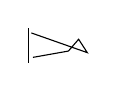
\begin{tikzpicture}
\draw (0,-.22)--(0,.22);
\draw (.04,.16)--(.75,-.09)--(.64,.08)--(.51,-.07)--(.06,-.15);
\end{tikzpicture}}}}

% 492-03: display (50).
\[
(50)\qquad \LMsourceMark{M000037}{\unsure{\widetilde{\mathcal T}_{1,1}}}
\longrightarrow \mathrm{GL}(2,\widehat{\mathbb Z})
\]

% 492-04: middle and lower paragraph.
and one should \var{\deleted{\LMsourceMark{M000038}{\unsure{be able to}}}}{\LMsourceMark{M000039}{\LMcancelledDoubts{\LMsourceMark{M000040}{\unsure{be able to}}}}}{deletion}{140-3-s492-D004} interpret this homomorphism
as the fundamental ``modular'' homomorphism of the theory of elliptic
curves (that the inverse image of \var{\deleted{$\LMsourceMark{M000041}{\unsure{\Gamma}}$}}{\LMsourceMark{M000042}{\LMcancelledDoubts{\(\LMsourceMark{M000043}{\unsure{\Gamma}}\)}}}{deletion}{140-3-s492-D005}
$\Gamma_{\mathbb Q}\subset\widetilde\Gamma_{\mathbb Q}$ in
$\LMsourceMark{M000044}{\unsure{\widetilde{\mathcal T}_{1,1}}}$ \LMsourceMark{M000045}{\unsure{can}} be interpreted as
$\LMsourceMark{M000046}{\unsure{\mathcal T_{1,1}}}\simeq\pi_1(M_{1,1\,\mathbb Q})$
must be more or less tautological, by construction.)

% 492-05: final paragraph, interlinear addition, and display (51).
It is clear in any case that the two coincide
\var{\inserted{for every $\gamma\in\widetilde M_{0,3}$}}{\LMadded{for every $\gamma\in\widetilde M_{0,3}$}}{insertion}{140-3-s492-I002}
\LMsourceMark{M000047}{\unsure{viewed}} \LMsourceMark{M000048}{\unsure{as|when}} elements of
\[
(51)\qquad \mu_2(\widehat{\mathbb Z})=\{\pm1\}^{\mathbb P}
\qquad (\mathbb P=\text{set of prime numbers})
\]
\LMsourceMark{M000049}{\mspage{491}}

\LMflushnotes\LMflushpages
\ifnum\LMform=1
\begin{LMapparatus}
\LMentry{140-3-s492-D001}{deletion}{\deleted{$\LMsourceMark{M000050}{\unsure{\Psi_{-\mathrm j}^{\pi}}}$}
}{\emph{\LMomittedlabel}}{Cancelled in the manuscript: omission follows the author's final state; uncertainty in the cancelled material remains marked.}{}
\LMentry{140-3-s492-D002}{deletion}{\deleted{\LMsourceMark{M000051}{\unsure{by}} \LMsourceMark{M000052}{\illegible{2}}}
}{\emph{\LMomittedlabel}}{Cancelled in the manuscript: omission follows the author's final state; uncertainty in the cancelled material remains marked.}{}
\LMentry{140-3-s492-D003}{deletion}{\deleted{\LMsourceMark{M000053}{\unsure{covering|profinite}} \LMsourceMark{M000054}{\unsure{with|of}} $\LMsourceMark{M000055}{\unsure{2}}$ \LMsourceMark{M000056}{\unsure{sheets}}}
}{\emph{\LMomittedlabel}}{Cancelled in the manuscript: omission follows the author's final state; uncertainty in the cancelled material remains marked.}{}
\LMentry{140-3-s492-I001}{insertion}{\inserted{ad-hoc extension}
}{\emph{\LMinsertedlabel}}{Explicit authorial insertion: integrated at the position recorded by the transcription, without changing its reading.}{}
\LMentry{140-3-s492-D004}{deletion}{\deleted{\LMsourceMark{M000057}{\unsure{be able to}}}
}{\emph{\LMomittedlabel}}{Cancelled in the manuscript: omission follows the author's final state; uncertainty in the cancelled material remains marked.}{}
\LMentry{140-3-s492-D005}{deletion}{\deleted{$\LMsourceMark{M000058}{\unsure{\Gamma}}$}
}{\emph{\LMomittedlabel}}{Cancelled in the manuscript: omission follows the author's final state; uncertainty in the cancelled material remains marked.}{}
\LMentry{140-3-s492-I002}{insertion}{\inserted{for every $\gamma\in\widetilde M_{0,3}$}
}{\emph{\LMinsertedlabel}}{Explicit authorial insertion: integrated at the position recorded by the transcription, without changing its reading.}{}
\end{LMapparatus}
\fi
\ifnum\LMform=2
\par\smallskip\begingroup\footnotesize\noindent\textcolor{gray}{\rule{.2\linewidth}{.35pt}}\par
\noindent\textit{\LMdoubtheading.}\par
\LMcarryover{140-3-s492-D001}{\(\LMsourceMark{M000059}{\unsure{\Psi_{-\mathrm j}^{\pi}}}\)
}
\LMcarryover{140-3-s492-D002}{\LMsourceMark{M000060}{\unsure{by}}\quad \LMsourceMark{M000061}{\illegible{2}}
}
\LMcarryover{140-3-s492-D003}{\LMsourceMark{M000062}{\unsure{covering|profinite}}\quad \LMsourceMark{M000063}{\unsure{with|of}}\quad \(\LMsourceMark{M000064}{\unsure{2}}\)\quad \LMsourceMark{M000065}{\unsure{sheets}}
}
\LMcarryover{140-3-s492-D004}{\LMsourceMark{M000066}{\unsure{be able to}}
}
\LMcarryover{140-3-s492-D005}{\(\LMsourceMark{M000067}{\unsure{\Gamma}}\)
}
\par\endgroup\smallskip
\fi

\LMsourceMark{M000068}{\scanpage{493}}
\LMsourceMark{M000069}{\mspage{549}}
% 493-01: continuation, with an overwritten source in the first display.
i.e. they coincide modulo a homomorphism
\[
\var{\deleted{\LMsourceMark{M000070}{\unsure{M_{0,3}}}}}{\LMsourceMark{M000071}{\LMcancelledDoubts{\(\LMsourceMark{M000072}{\unsure{M_{0,3}}}\)}}}{deletion}{140-3-s493-D001}\var{\inserted{\LMsourceMark{M000073}{\unsure{\widetilde\Gamma_{\mathbb Q}}}}}{\LMadded{\LMsourceMark{M000074}{\unsure{\widetilde\Gamma_{\mathbb Q}}}}}{insertion}{140-3-s493-I001}
\longrightarrow\mu_2(\widehat{\mathbb Z})\simeq\{\pm1\}^{\mathbb P}
\]
i.e. a homomorphism
\[
\begin{aligned}
G_{\mathrm m}(\widehat{\mathbb Z})_2
&=(\widehat{\mathbb Z}^{*})_2\simeq\{\pm1\}^{\mathbb P}
\longrightarrow\var{\deleted{\LMsourceMark{M000075}{\unsure{\mu}}}}{\LMsourceMark{M000076}{\LMcancelledDoubts{\(\LMsourceMark{M000077}{\unsure{\mu}}\)}}}{deletion}{140-3-s493-D002}\LMsourceMark{M000078}{\unsure{{}_2G_{\mathrm m}}}(\widehat{\mathbb Z})
=\mu_2(\widehat{\mathbb Z})\\
&\hspace{24em}\simeq\{\pm1\}^{\mathbb P}
\end{aligned}
\]

% 493-02: middle prose.
--- so it is not a \LMsourceMark{M000079}{\unsure{certain}} indeterminacy that is at issue!
It is morally certain that the two coincide --- I have not tried to
prove it.

% 493-03: lower prose and its interlinear insertion.
As for (35) (36), they must surely correspond to the action of
$\Gamma_{\mathbb Q}$ on the Tate modules of elliptic curves with
exceptional isomorphisms, corresponding precisely to the points
$(1/2,2,-1)$ and $(-\overline{\mathrm j},-\mathrm j)$ of
$M_{0,3\,\mathbb Q}=M_{1,1}[2]'_{\mathbb Q}$.
The indeterminacy of sign \var{\inserted{\LMsourceMark{M000080}{\unsure{must|of which}}}}{\LMadded{\LMsourceMark{M000081}{\unsure{must|of which}}}}{insertion}{140-3-s493-I002} \LMsourceMark{M000082}{\unsure{correspond|corresponds}} to the indeterminacy
in lifting a point of $M_{1,1}[2]'_{\mathbb Q}$ to a point of
$M_{1,1}[2]_{\mathbb Q}$, i.e. in choosing an elliptic curve
(with ``\uline{rigidification}'' of level 2) corresponding to the
\uline{Legendre} data $(0,1,\infty,\LMsourceMark{M000083}{\unsure{q|\rho}})$ with
$\LMsourceMark{M000084}{\unsure{\rho|q}}=1/2$ or $\LMsourceMark{M000085}{\unsure{\rho|q}}=-\overline{\mathrm j}$.
\LMsourceMark{M000086}{\mspage{492}}

\LMflushnotes\LMflushpages
\ifnum\LMform=1
\begin{LMapparatus}
\LMentry{140-3-s493-D001}{deletion}{\(\deleted{\LMsourceMark{M000087}{\unsure{M_{0,3}}}}\)
}{\emph{\LMomittedlabel}}{Cancelled in the manuscript: omission follows the author's final state; uncertainty in the cancelled material remains marked.}{}
\LMentry{140-3-s493-I001}{insertion}{\(\inserted{\LMsourceMark{M000088}{\unsure{\widetilde\Gamma_{\mathbb Q}}}}\)
}{\emph{\LMinsertedlabel}}{Explicit authorial insertion: integrated at the position recorded by the transcription, without changing its reading.}{}
\LMentry{140-3-s493-D002}{deletion}{\(\deleted{\LMsourceMark{M000089}{\unsure{\mu}}}\)
}{\emph{\LMomittedlabel}}{Cancelled in the manuscript: omission follows the author's final state; uncertainty in the cancelled material remains marked.}{}
\LMentry{140-3-s493-I002}{insertion}{\inserted{\LMsourceMark{M000090}{\unsure{must|of which}}}
}{\emph{\LMinsertedlabel}}{Explicit authorial insertion: integrated at the position recorded by the transcription, without changing its reading.}{}
\end{LMapparatus}
\fi
\ifnum\LMform=2
\par\smallskip\begingroup\footnotesize\noindent\textcolor{gray}{\rule{.2\linewidth}{.35pt}}\par
\noindent\textit{\LMdoubtheading.}\par
\LMcarryover{140-3-s493-D001}{\(\LMsourceMark{M000091}{\unsure{M_{0,3}}}\)
}
\LMcarryover{140-3-s493-D002}{\(\LMsourceMark{M000092}{\unsure{\mu}}\)
}
\par\endgroup\smallskip
\fi

\LMsourceMark{M000093}{\scanpage{494}}
% 494-01: upper paragraph.
Even once the \LMsourceMark{M000094}{\unsure{ambiguity}} of sign for
$\Theta_{\LMsourceMark{M000095}{\unsure{G}}}^{\LMsourceMark{M000096}{\unsure{\pi}}}$ is removed by passing to the two-sheeted extension
$\LMsourceMark{M000097}{\unsure{\widetilde{\mathcal T}_{1,1}}}$ of
$\widetilde M_{0,3}$, the indeterminacy of the signs for
$\Theta_{\rho}^{\LMsourceMark{M000098}{\unsure{\pi}}},\Theta_{\sigma}^{\LMsourceMark{M000099}{\unsure{\pi}}}$
is not \LMsourceMark{M000100}{\unsure{removed}} for all that, for the splittings
\var{\deleted{$\LMsourceMark{M000101}{\unsure{\Psi_{\rho}^{\pi},\Psi_{\sigma}^{\pi}}}$}}{\LMsourceMark{M000102}{\LMcancelledDoubts{\(\LMsourceMark{M000103}{\unsure{\Psi_{\rho}^{\pi},\Psi_{\sigma}^{\pi}}}\)}}}{deletion}{140-3-s494-D001}
$\Psi_{1/2}^{\LMsourceMark{M000104}{\unsure{\pi}}},\Psi_{-\overline{\mathrm j}}^{\LMsourceMark{M000105}{\unsure{\pi}}}$)
are not for all that splittings (even partial!)
of \var{\deleted{\LMsourceMark{M000106}{\unsure{this}}}}{\LMsourceMark{M000107}{\LMcancelledDoubts{\LMsourceMark{M000108}{\unsure{this}}}}}{deletion}{140-3-s494-D002} \LMsourceMark{M000109}{\unsure{the extension}}
$\LMsourceMark{M000110}{\unsure{\widetilde{\mathcal T}_{1,1}}}$, but only of
$\widetilde M_{0,3}$ --- and lifting them to splittings of
$\LMsourceMark{M000111}{\unsure{\widetilde{\mathcal T}_{1,1}}}$
\var{\inserted{over $\LMsourceMark{M000112}{\unsure{\mathcal T_{1,1}}}$,}}{\LMadded{over $\LMsourceMark{M000113}{\unsure{\mathcal T_{1,1}}}$,}}{insertion}{140-3-s494-I001}
amounts, very precisely, to choosing precisely elliptic curves with
Legendre rigidification over the points $1/2,-\overline{\mathrm j}$.
Thus, calculations made in terms of automorphisms of the groups with loops
$\widehat\Pi_{0,3}$ \LMsourceMark{M000114}{\unsure{or}} \var{\inserted{of}}{\LMadded{of}}{insertion}{140-3-s494-I002}
$\LMsourceMark{M000115}{\unsure{\mathcal{C}}}_{0,3}^{+\wedge}$,
\LMsourceMark{M000116}{\unsure{give back}} \var{\inserted{(without having \LMsourceMark{M000117}{\unsure{looked for}} them!)}}{\LMadded{(without having \LMsourceMark{M000118}{\unsure{looked for}} them!)}}{insertion}{140-3-s494-I003}
results that fit very closely with particularly crucial
arithmetico-geometric truths.
\LMsourceMark{M000119}{\mspage{493}}

\Needspace{6\baselineskip}

\LMflushnotes\LMflushpages
\ifnum\LMform=1
\begin{LMapparatus}
\LMentry{140-3-s494-D001}{deletion}{\deleted{$\LMsourceMark{M000120}{\unsure{\Psi_{\rho}^{\pi},\Psi_{\sigma}^{\pi}}}$}
}{\emph{\LMomittedlabel}}{Cancelled in the manuscript: omission follows the author's final state; uncertainty in the cancelled material remains marked.}{}
\LMentry{140-3-s494-D002}{deletion}{\deleted{\LMsourceMark{M000121}{\unsure{this}}}
}{\emph{\LMomittedlabel}}{Cancelled in the manuscript: omission follows the author's final state; uncertainty in the cancelled material remains marked.}{}
\LMentry{140-3-s494-I001}{insertion}{\inserted{over $\LMsourceMark{M000122}{\unsure{\mathcal T_{1,1}}}$,}
}{\emph{\LMinsertedlabel}}{Explicit authorial insertion: integrated at the position recorded by the transcription, without changing its reading.}{}
\LMentry{140-3-s494-I002}{insertion}{\inserted{of}
}{\emph{\LMinsertedlabel}}{Explicit authorial insertion: integrated at the position recorded by the transcription, without changing its reading.}{}
\LMentry{140-3-s494-I003}{insertion}{\inserted{(without having \LMsourceMark{M000123}{\unsure{looked for}} them!)}
}{\emph{\LMinsertedlabel}}{Explicit authorial insertion: integrated at the position recorded by the transcription, without changing its reading.}{}
\end{LMapparatus}
\fi
\ifnum\LMform=2
\par\smallskip\begingroup\footnotesize\noindent\textcolor{gray}{\rule{.2\linewidth}{.35pt}}\par
\noindent\textit{\LMdoubtheading.}\par
\LMcarryover{140-3-s494-D001}{\(\LMsourceMark{M000124}{\unsure{\Psi_{\rho}^{\pi},\Psi_{\sigma}^{\pi}}}\)
}
\LMcarryover{140-3-s494-D002}{\LMsourceMark{M000125}{\unsure{this}}
}
\par\endgroup\smallskip
\fi

\LMsourceMark{M000126}{\scanpage{495}}
\LMsourceMark{M000127}{\mspage{550}}
% 495-01: heading.
49.\quad \uline{Homomorphisms of} $M_{0,3}$, the general groups
$M_{\rho,\sigma}$.

% 495-02: left-margin notes.
\LMsourceMark{M000128}{\margin{\LMsourceMark{M000129}{\unsure{Where we get our feet wet}}\ldots}}
\LMsourceMark{M000130}{\margin{\LMsourceMark{M000131}{\unsure{All of}} this section \var{\inserted{I}}{\LMadded{I}}{insertion}{140-3-s495-I001} \LMsourceMark{M000132}{\unsure{seems}}
entirely useless for what follows, it is a preliminary \LMsourceMark{M000133}{\unsure{groping}}
to lead into section \uline{II} page 553.}}

% 495-03: first paragraph.
I) Consider a \var{\inserted{closed}}{\LMadded{closed}}{insertion}{140-3-s495-I002} subgroup $G$ of $M_{0,3}$,
containing $\LMsourceMark{M000134}{\unsure{\mathcal C}}_{0,3}^{+\wedge}$, hence the inverse image of a
closed subgroup of $\widetilde\Gamma_{0,3}$.
We assume that the latter is ``big enough'' --- say that it contains
a subgroup of finite index in
$\Gamma_{\mathbb Q}\subset\widetilde\Gamma_{0,3}$.
For the moment, we assume for simplicity that $G\subset\operatorname{Ker}\varepsilon_3$.
In summary
\[
(1)\qquad
\LMsourceMark{M000135}{\unsure{\mathcal C}}_{0,3}^{+\wedge}\subset G\subset\widetilde M_{0,3},
\qquad u\in G\Longrightarrow\mu(u)\equiv1\ (3).
\]

% 495-04: interlinear correction and parallel maps.
This last hypothesis thus \var{\deleted{implies}}{}{deletion}{140-3-s495-D001}\var{\inserted{means}}{\LMadded{means}}{insertion}{140-3-s495-I003} that
for every $u\in G$, we have $\alpha_0(u)\in\LMsourceMark{M000136}{\unsure{\mathcal C}}_{0,3}^{\wedge+}$,
so we have
\[
(\LMsourceMark{M000137}{\unsure{2}})\qquad
\diagram{\begin{tikzcd}[ampersand replacement=\&,column sep=large]
G \arrow[r,shift left=.7ex,"\underline{\alpha}_0"]
  \arrow[r,shift right=.7ex,"\underline{\beta}_0"']
\& \LMsourceMark{M000138}{\unsure{\mathcal C}}_{0,3}^{+}
\end{tikzcd}},
\]
characterized by
\[
(2')\qquad
\left\{\begin{aligned}
u(\rho)&=\operatorname{int}(\alpha_0)\rho\\
u(\sigma)&=\operatorname{int}(\beta_0)\sigma
\end{aligned}\right.
\qquad
\begin{aligned}
\alpha_0&=\underline{\alpha}_0(u)\\
\beta_0&=\underline{\beta}_0(u).
\end{aligned}
\]

% 495-05: the vertically arranged subgroups, including the intervening sign.
We consider
\[
(3)\qquad
\begin{array}{l}
G(0)=G\cap\widetilde M_{0,3}(0)\\[-.4em]
\quad\cap\\[-.4em]
G[0]=G\cap\widetilde M_{0,3}[0]=\operatorname{Norm}_{G}(L_0^{\LMsourceMark{M000139}{\unsure{\mathcal C}}})
\end{array}
\]
so that
\[
\begin{aligned}
(4)\qquad&G=G(0).\LMsourceMark{M000140}{\unsure{\mathcal C}}_{0,3}^{+\wedge}
&&\text{(semidirect product)}\\
(5)\qquad&G[0]=G(0).L_0^{\LMsourceMark{M000141}{\unsure{\mathcal C}}}
&&\text{id}\\
(6)\qquad&G[0]\cap\LMsourceMark{M000142}{\unsure{\mathcal C}}_{0,3}^{+\wedge}
=L_0^{\LMsourceMark{M000143}{\unsure{\mathcal C}}}.
\end{aligned}
\]

% 495-06: definition (7) and last line.
We have set
\[
(7)\qquad
\begin{gathered}
L_0^{\LMsourceMark{M000144}{\unsure{\mathcal C}}}=\text{closed subgroup of }
\LMsourceMark{M000145}{\unsure{\mathcal C}}_{0,3}^{+\wedge}\text{ generated}\\
\text{by }\varepsilon_0
\end{gathered}
\]
and we define likewise $L_1^{\LMsourceMark{M000146}{\unsure{\mathcal C}}},L_{\infty}^{\LMsourceMark{M000147}{\unsure{\mathcal C}}}$.
\LMsourceMark{M000148}{\mspage{494}}

\LMflushnotes\LMflushpages
\ifnum\LMform=1
\begin{LMapparatus}
\LMentry{140-3-s495-I001}{insertion}{\inserted{I}
}{\emph{\LMinsertedlabel}}{Explicit authorial insertion: integrated at the position recorded by the transcription, without changing its reading.}{}
\LMentry{140-3-s495-I002}{insertion}{\inserted{closed}
}{\emph{\LMinsertedlabel}}{Explicit authorial insertion: integrated at the position recorded by the transcription, without changing its reading.}{}
\LMentry{140-3-s495-D001}{deletion}{\deleted{implies}
}{\emph{\LMomittedlabel}}{Cancelled in the manuscript: omission follows the author's final state; uncertainty in the cancelled material remains marked.}{}
\LMentry{140-3-s495-I003}{insertion}{\inserted{means}
}{\emph{\LMinsertedlabel}}{Explicit authorial insertion: integrated at the position recorded by the transcription, without changing its reading.}{}
\end{LMapparatus}
\fi

\LMsourceMark{M000149}{\scanpage{496}}
% 496-01: paragraph and first map, with changes of target notation.
Consider a \var{\inserted{profinite}}{\LMadded{profinite}}{insertion}{140-3-s496-I001} group
$\var{\deleted{\LMsourceMark{M000150}{\unsure{A}}}}{\LMsourceMark{M000151}{\LMcancelledDoubts{\(\LMsourceMark{M000152}{\unsure{A}}\)}}}{deletion}{140-3-s496-D001}\var{\inserted{M}}{\LMadded{M}}{insertion}{140-3-s496-I002}$, and a \var{\inserted{(continuous)}}{\LMadded{(continuous)}}{insertion}{140-3-s496-I003}
\uline{surjective} homomorphism
\[
(8)\qquad \varphi:G\longrightarrow\var{\deleted{\LMsourceMark{M000153}{\unsure{A}}}}{\LMsourceMark{M000154}{\LMcancelledDoubts{\(\LMsourceMark{M000155}{\unsure{A}}\)}}}{deletion}{140-3-s496-D002}M.
\]
We set
\[
(9)\quad
\left\{\begin{aligned}
\varphi(\LMsourceMark{M000156}{\unsure{\mathcal C}}_{0,3}^{+\wedge})
 &=\LMsourceMark{M000157}{\unsure{\mathcal C}}\qquad\text{normal subgroup of }M\\
\varphi(G(0))&=\var{\deleted{\LMsourceMark{M000158}{\unsure{A}}}}{\LMsourceMark{M000159}{\LMcancelledDoubts{\(\LMsourceMark{M000160}{\unsure{A}}\)}}}{deletion}{140-3-s496-D003}\var{\inserted{M}}{\LMadded{M}}{insertion}{140-3-s496-I004}(0)\\
\varphi(G[0])&=\var{\deleted{\LMsourceMark{M000161}{\unsure{A}}}}{\LMsourceMark{M000162}{\LMcancelledDoubts{\(\LMsourceMark{M000163}{\unsure{A}}\)}}}{deletion}{140-3-s496-D004}\var{\inserted{M}}{\LMadded{M}}{insertion}{140-3-s496-I005}[0].\\
\varphi(L_0^{\LMsourceMark{M000164}{\unsure{\mathcal C}}})&=L_0^{\var{\deleted{\LMsourceMark{M000165}{\unsure{\mathcal C}}}}{\LMsourceMark{M000166}{\LMcancelledDoubts{\(\LMsourceMark{M000167}{\unsure{\mathcal C}}\)}}}{deletion}{140-3-s496-D005}}
\end{aligned}\right.
\]

% 496-02: subgroup relations.
\var{\deleted{\LMsourceMark{M000168}{\unsure{Thus}}}}{\LMsourceMark{M000169}{\LMcancelledDoubts{\LMsourceMark{M000170}{\unsure{Thus}}}}}{deletion}{140-3-s496-D006}

Thus these are closed subgroups of $M$, satisfying
\[
\begin{aligned}
(10)\qquad&M(0)\subset M[0]\subset\operatorname{Norm}_{M}(L_0)\\
(11)\qquad&L_0^{\var{\deleted{\LMsourceMark{M000171}{\unsure{\mathcal C}}}}{\LMsourceMark{M000172}{\LMcancelledDoubts{\(\LMsourceMark{M000173}{\unsure{\mathcal C}}\)}}}{deletion}{140-3-s496-D007}}
\subset\LMsourceMark{M000174}{\unsure{\mathcal C}}\cap M[0].
\end{aligned}
\]

% 496-03: the surviving generator relations.
By abuse of language, we still denote by $\rho,\sigma,\varepsilon_0,\varepsilon_1$
\ldots\ the images of these elements in $\LMsourceMark{M000175}{\unsure{\mathcal C}}$, which
therefore satisfy there the relations known in $\LMsourceMark{M000176}{\unsure{\mathcal C}}_{0,3}^{+\wedge}$,
in particular
\[
(12)\qquad
\sigma^2=\rho^3=1,\qquad
\sigma\rho=\varepsilon_0,\quad \rho\sigma=\varepsilon_1,\qquad
\varepsilon_1=\sigma(\varepsilon_0)=\rho(\varepsilon_0).
\]

% 496-04: paragraph and revised definition (13).
The restrictions of the maps $\alpha_0,\beta_0$ of (2,2') to
$M_{\rho,\sigma}[0]$ will rather be denoted $\alpha,\beta$, where $\alpha,\beta$
are in fact maps
\[
(13)\quad
\diagram{\begin{tikzcd}[ampersand replacement=\&,column sep=large]
{\begin{gathered}
SG\overset{\mathrm{dfn}}=\var{\deleted{\text{extension of}}}{}{deletion}{140-3-s496-D008}\ G\\
\text{by }L_0^{\LMsourceMark{M000177}{\unsure{\mathcal C}}},\ \text{inverse}\\
\text{image of }\LMsourceMark{M000178}{\unsure{G}}\\
\text{in }S\widetilde M_{0,3}\\
=\{(u,f)\in G\times\LMsourceMark{M000179}{\unsure{\mathcal C}}_{0,3}^{+\wedge}\mid fu\in G[0]
\end{gathered}}
\arrow[r,shift left=.7ex,"\alpha"]
\arrow[r,shift right=.7ex,"\beta"']
\&\LMsourceMark{M000180}{\unsure{\mathcal C}}_{0,3}^{+\wedge}
\end{tikzcd}}
\]
of which we look at the restrictions to the \uline{subgroup}
($\simeq M_{\rho,\sigma}[0]$) of $SG$ defined by the relation $f=1$.

% 496-05: composition of the two functions, and (14).
Composing $\underline\alpha,\underline\beta:$
\diagram{\begin{tikzcd}[ampersand replacement=\&,column sep=small]
\var{\deleted{\LMsourceMark{M000181}{\unsure{M[0]}}}}{\LMsourceMark{M000182}{\LMcancelledDoubts{\(\LMsourceMark{M000183}{\unsure{M[0]}}\)}}}{deletion}{140-3-s496-D009}\var{\inserted{G[0]}}{\LMadded{G[0]}}{insertion}{140-3-s496-I006}
\arrow[r,shift left=.5ex]\arrow[r,shift right=.5ex]
\&\LMsourceMark{M000184}{\unsure{\mathcal C}}_{0,3}^{+\wedge}
\end{tikzcd}}
with $\varphi\mid\LMsourceMark{M000185}{\unsure{\mathcal C}}_{0,3}^{+\wedge}$, we find
maps, again denoted $\underline\alpha,\underline\beta$
(where $\underline\alpha^M,\underline\beta^M$ in case of possible confusion)
\[
(14)\qquad
\diagram{\begin{tikzcd}[ampersand replacement=\&,column sep=large]
G[0]\arrow[r,shift left=.7ex,"\underline\alpha"]
\arrow[r,shift right=.7ex,"\underline\beta"']
\&\LMsourceMark{M000186}{\unsure{\mathcal C}}
\end{tikzcd}}
\]
thus satisfying
\[
(15)\qquad
\left\{\begin{aligned}
\LMsourceMark{M000187}{\unsure{u}}(\rho)&=\operatorname{int}(\alpha)\rho\\
\LMsourceMark{M000188}{\unsure{u}}(\sigma)&=\operatorname{int}(\beta)\sigma
\end{aligned}\right.
\qquad
\begin{gathered}
\text{for }u\in M[0]\ \var{\inserted{\text{\LMsourceMark{M000189}{\unsure{of}}}}}{\LMadded{\text{\LMsourceMark{M000190}{\unsure{of}}}}}{insertion}{140-3-s496-I007}\text{ the form }\varphi(u_0),\\
\text{and }\alpha=\underline\alpha(u_0),\ \beta=\underline\beta(u_0).
\end{gathered}
\]
\LMsourceMark{M000191}{\mspage{495}}

\LMflushnotes\LMflushpages
\ifnum\LMform=1
\begin{LMapparatus}
\LMentry{140-3-s496-I001}{insertion}{\inserted{profinite}
}{\emph{\LMinsertedlabel}}{Explicit authorial insertion: integrated at the position recorded by the transcription, without changing its reading.}{}
\LMentry{140-3-s496-D001}{deletion}{\(\deleted{\LMsourceMark{M000192}{\unsure{A}}}\)
}{\emph{\LMomittedlabel}}{Cancelled in the manuscript: omission follows the author's final state; uncertainty in the cancelled material remains marked.}{}
\LMentry{140-3-s496-I002}{insertion}{\(\inserted{M}\)
}{\emph{\LMinsertedlabel}}{Explicit authorial insertion: integrated at the position recorded by the transcription, without changing its reading.}{}
\LMentry{140-3-s496-I003}{insertion}{\inserted{(continuous)}
}{\emph{\LMinsertedlabel}}{Explicit authorial insertion: integrated at the position recorded by the transcription, without changing its reading.}{}
\LMentry{140-3-s496-D002}{deletion}{\(\deleted{\LMsourceMark{M000193}{\unsure{A}}}\)
}{\emph{\LMomittedlabel}}{Cancelled in the manuscript: omission follows the author's final state; uncertainty in the cancelled material remains marked.}{}
\LMentry{140-3-s496-D003}{deletion}{\(\deleted{\LMsourceMark{M000194}{\unsure{A}}}\)
}{\emph{\LMomittedlabel}}{Cancelled in the manuscript: omission follows the author's final state; uncertainty in the cancelled material remains marked.}{}
\LMentry{140-3-s496-I004}{insertion}{\(\inserted{M}\)
}{\emph{\LMinsertedlabel}}{Explicit authorial insertion: integrated at the position recorded by the transcription, without changing its reading.}{}
\LMentry{140-3-s496-D004}{deletion}{\(\deleted{\LMsourceMark{M000195}{\unsure{A}}}\)
}{\emph{\LMomittedlabel}}{Cancelled in the manuscript: omission follows the author's final state; uncertainty in the cancelled material remains marked.}{}
\LMentry{140-3-s496-I005}{insertion}{\(\inserted{M}\)
}{\emph{\LMinsertedlabel}}{Explicit authorial insertion: integrated at the position recorded by the transcription, without changing its reading.}{}
\LMentry{140-3-s496-D005}{deletion}{\(\deleted{\LMsourceMark{M000196}{\unsure{\mathcal C}}}\)
}{\emph{\LMomittedlabel}}{Cancelled in the manuscript: omission follows the author's final state; uncertainty in the cancelled material remains marked.}{}
\LMentry{140-3-s496-D006}{deletion}{\deleted{\LMsourceMark{M000197}{\unsure{Thus}}}
}{\emph{\LMomittedlabel}}{Cancelled in the manuscript: omission follows the author's final state; uncertainty in the cancelled material remains marked.}{}
\LMentry{140-3-s496-D007}{deletion}{\(\deleted{\LMsourceMark{M000198}{\unsure{\mathcal C}}}\)
}{\emph{\LMomittedlabel}}{Cancelled in the manuscript: omission follows the author's final state; uncertainty in the cancelled material remains marked.}{}
\LMentry{140-3-s496-D008}{deletion}{\(\deleted{\text{extension of}}\)
}{\emph{\LMomittedlabel}}{Cancelled in the manuscript: omission follows the author's final state; uncertainty in the cancelled material remains marked.}{}
\LMentry{140-3-s496-D009}{deletion}{\(\deleted{\LMsourceMark{M000199}{\unsure{M[0]}}}\)
}{\emph{\LMomittedlabel}}{Cancelled in the manuscript: omission follows the author's final state; uncertainty in the cancelled material remains marked.}{}
\LMentry{140-3-s496-I006}{insertion}{\(\inserted{G[0]}\)
}{\emph{\LMinsertedlabel}}{Explicit authorial insertion: integrated at the position recorded by the transcription, without changing its reading.}{}
\LMentry{140-3-s496-I007}{insertion}{\(\inserted{\text{\LMsourceMark{M000200}{\unsure{of}}}}\)
}{\emph{\LMinsertedlabel}}{Explicit authorial insertion: integrated at the position recorded by the transcription, without changing its reading.}{}
\end{LMapparatus}
\fi
\ifnum\LMform=2
\par\smallskip\begingroup\footnotesize\noindent\textcolor{gray}{\rule{.2\linewidth}{.35pt}}\par
\noindent\textit{\LMdoubtheading.}\par
\LMcarryover{140-3-s496-D001}{\(\LMsourceMark{M000201}{\unsure{A}}\)
}
\LMcarryover{140-3-s496-D002}{\(\LMsourceMark{M000202}{\unsure{A}}\)
}
\LMcarryover{140-3-s496-D003}{\(\LMsourceMark{M000203}{\unsure{A}}\)
}
\LMcarryover{140-3-s496-D004}{\(\LMsourceMark{M000204}{\unsure{A}}\)
}
\LMcarryover{140-3-s496-D005}{\(\LMsourceMark{M000205}{\unsure{\mathcal C}}\)
}
\LMcarryover{140-3-s496-D006}{\LMsourceMark{M000206}{\unsure{Thus}}
}
\LMcarryover{140-3-s496-D007}{\(\LMsourceMark{M000207}{\unsure{\mathcal C}}\)
}
\LMcarryover{140-3-s496-D009}{\(\LMsourceMark{M000208}{\unsure{M[0]}}\)
}
\par\endgroup\smallskip
\fi

\LMsourceMark{M000209}{\scanpage{497}}
\LMsourceMark{M000210}{\mspage{551}}

% 497-01
A priori, $\alpha$ and $\beta$ depend on the choice of $u_0$ from which $u$ comes
not only on $u$ --- but
% 497-02
\[
(16)\qquad
\left\{\begin{aligned}
\alpha\rho(\alpha)^{-1}&=[u,\rho]\\
\beta\sigma(\beta)^{-1}&=[u,\sigma]
\end{aligned}\right.
\]
% 497-03
do not depend on it. If we put
% 497-04
\[
(17)\qquad
T_{\rho}=\uline{\mathrm{Centr}}_M(\rho)
\qquad
T_{\sigma}=\uline{\mathrm{Centr}}_M(\sigma)
\]
% 497-05
we thus see that, modulo $T_{\rho}$ resp. $T_{\sigma}$,
$\alpha,\beta$ depend only on $u$.

% 497-06, 497-07, 497-08, 497-09
\uline{Hypothesis}
$\alpha\var{\inserted{{}=\alpha(u_0)}}{\LMadded{{}=\alpha(u_0)}}{insertion}{140-3-s497-I001},\beta\var{\inserted{{}=\beta(u_0)}}{\LMadded{{}=\beta(u_0)}}{insertion}{140-3-s497-I002}$
depend only on $u=\varphi(u_0)$
(for $u_0\in\var{\deleted{\LMsourceMark{M000211}{\unsure{M}}}}{\LMsourceMark{M000212}{\LMcancelledDoubts{\(\LMsourceMark{M000213}{\unsure{M}}\)}}}{deletion}{140-3-s497-D001}\LMsourceMark{M000214}{\unsure{G}}[0]$).

% 497-10
We shall \LMsourceMark{M000215}{\unsure{express}} this hypothesis in a slightly different way,
by introducing
% 497-11
\[
(18)\qquad J=\operatorname{Ker}(G[0]\longrightarrow M[0]),
\]
% 497-12, 497-13
we thus want that for $\var{\deleted{\LMsourceMark{M000216}{\unsure{\alpha}}}}{\LMsourceMark{M000217}{\LMcancelledDoubts{\(\LMsourceMark{M000218}{\unsure{\alpha}}\)}}}{deletion}{140-3-s497-D002}$
% 497-14, 497-15
\[
u'_0=\var{\deleted{u_0}}{}{deletion}{140-3-s497-D003}\delta_0u_0\quad
\text{with }u_0\in G[0],\ \delta_0\in J,\quad\text{we have}
\]
% 497-16
\[
\alpha(u'_0)=\alpha(u_0),\qquad \beta(u'_0)=\beta(u_0)
\]
% 497-17, 497-18
\LMsourceMark{M000219}{\unsure{Write}}
\[
\begin{gathered}
\alpha_0=\uline{\alpha}(u_0),\quad
\beta_0=\uline{\beta}(u_0),\quad
\alpha'_0=\uline{\alpha}(u'_0),\quad
\beta'_0=\uline{\beta}(u'_0),\quad
\overline{\alpha}_0=\uline{\alpha}(\delta_0),\quad
\overline{\beta}_0=\uline{\beta}(\LMsourceMark{M000220}{\unsure{\delta_1|\delta_0}}),
\end{gathered}
\]
\uline{in} $G$, so that we shall have, by the cocycle formulas of $G$
% 497-19
\[
\alpha'_0=\delta_0(\alpha_0)\overline{\alpha}_0,
\qquad
\beta'_0=\delta_0(\beta_0)\overline{\beta}_0,
\]
% 497-20
whence, applying $\varphi$ and noting that
% 497-21
\[
\begin{aligned}
\varphi(\delta_0(\alpha_0))
&=\underbrace{\varphi(\delta_0)}_{1}(\varphi(\alpha_0))
=\varphi(\alpha_0)\overset{\mathrm{dfn}}=\alpha
&&\text{and likewise}\\
\varphi(\delta_0(\beta_0))&=\varphi(\beta_0)\overset{\mathrm{dfn}}=\beta
\end{aligned}
\]
% 497-22, 497-23
\[
(19)\qquad
\alpha'=\var{\deleted{\LMsourceMark{M000221}{\unsure{\varphi}}}}{\LMsourceMark{M000222}{\LMcancelledDoubts{\(\LMsourceMark{M000223}{\unsure{\varphi}}\)}}}{deletion}{140-3-s497-D004}\alpha\overline{\alpha},\qquad
\beta'=\beta\overline{\beta}\qquad\text{in }\LMsourceMark{M000224}{\unsure{\mathcal{C}}}
\]
% 497-24, 497-25
where $\alpha,\beta,\alpha',\beta',\overline{\alpha},\overline{\beta}$ are the images under
$\varphi$ of the quantities $\alpha_0$ etc in $\LMsourceMark{M000225}{\unsure{\mathcal{C}}}_{0,3}^{+\wedge}$.
\var{\deleted{\LMsourceMark{M000226}{\unsure{with}} $\alpha=\alpha(u_0)$}}{\LMsourceMark{M000227}{\LMcancelledDoubts{\LMsourceMark{M000228}{\unsure{with}}}}}{deletion}{140-3-s497-D005}
Thus the hypothesis means this
% 497-26
\[
(20)\qquad
\forall\,\delta_0\in J\overset{\mathrm{dfn}}=
\operatorname{Ker}(G[0]\longrightarrow M[0]),\quad
\text{we have}\quad
\LMsourceMark{M000229}{\unsure{\alpha^{\Pi}}}(\delta_0),\LMsourceMark{M000230}{\unsure{\beta^{\Pi}}}(\delta_0)
\in\LMsourceMark{M000231}{\unsure{\operatorname{Ker}}}\varphi
\]
% 497-27, 497-28
\var{\deleted{\LMsourceMark{M000232}{\unsure{when}}}}{\LMsourceMark{M000233}{\LMcancelledDoubts{\LMsourceMark{M000234}{\unsure{when}}}}}{deletion}{140-3-s497-D006}
When this hypothesis is satisfied, we thus have maps
\LMsourceMark{M000235}{\mspage{496}}

\LMflushnotes\LMflushpages
\ifnum\LMform=1
\begin{LMapparatus}
\LMentry{140-3-s497-I001}{insertion}{\(\inserted{{}=\alpha(u_0)}\)
}{\emph{\LMinsertedlabel}}{Explicit authorial insertion: integrated at the position recorded by the transcription, without changing its reading.}{}
\LMentry{140-3-s497-I002}{insertion}{\(\inserted{{}=\beta(u_0)}\)
}{\emph{\LMinsertedlabel}}{Explicit authorial insertion: integrated at the position recorded by the transcription, without changing its reading.}{}
\LMentry{140-3-s497-D001}{deletion}{\(\deleted{\LMsourceMark{M000236}{\unsure{M}}}\)
}{\emph{\LMomittedlabel}}{Cancelled in the manuscript: omission follows the author's final state; uncertainty in the cancelled material remains marked.}{}
\LMentry{140-3-s497-D002}{deletion}{\(\deleted{\LMsourceMark{M000237}{\unsure{\alpha}}}\)
}{\emph{\LMomittedlabel}}{Cancelled in the manuscript: omission follows the author's final state; uncertainty in the cancelled material remains marked.}{}
\LMentry{140-3-s497-D003}{deletion}{\(\deleted{u_0}\)
}{\emph{\LMomittedlabel}}{Cancelled in the manuscript: omission follows the author's final state; uncertainty in the cancelled material remains marked.}{}
\LMentry{140-3-s497-D004}{deletion}{\(\deleted{\LMsourceMark{M000238}{\unsure{\varphi}}}\)
}{\emph{\LMomittedlabel}}{Cancelled in the manuscript: omission follows the author's final state; uncertainty in the cancelled material remains marked.}{}
\LMentry{140-3-s497-D005}{deletion}{\deleted{\LMsourceMark{M000239}{\unsure{with}} $\alpha=\alpha(u_0)$}
}{\emph{\LMomittedlabel}}{Cancelled in the manuscript: omission follows the author's final state; uncertainty in the cancelled material remains marked.}{}
\LMentry{140-3-s497-D006}{deletion}{\deleted{\LMsourceMark{M000240}{\unsure{when}}}
}{\emph{\LMomittedlabel}}{Cancelled in the manuscript: omission follows the author's final state; uncertainty in the cancelled material remains marked.}{}
\end{LMapparatus}
\fi
\ifnum\LMform=2
\par\smallskip\begingroup\footnotesize\noindent\textcolor{gray}{\rule{.2\linewidth}{.35pt}}\par
\noindent\textit{\LMdoubtheading.}\par
\LMcarryover{140-3-s497-D001}{\(\LMsourceMark{M000241}{\unsure{M}}\)
}
\LMcarryover{140-3-s497-D002}{\(\LMsourceMark{M000242}{\unsure{\alpha}}\)
}
\LMcarryover{140-3-s497-D004}{\(\LMsourceMark{M000243}{\unsure{\varphi}}\)
}
\LMcarryover{140-3-s497-D005}{\LMsourceMark{M000244}{\unsure{with}}
}
\LMcarryover{140-3-s497-D006}{\LMsourceMark{M000245}{\unsure{when}}
}
\par\endgroup\smallskip
\fi

\LMsourceMark{M000246}{\scanpage{498}}

% 498-01
\[
(21)\qquad
\diagram{\begin{tikzcd}[ampersand replacement=\&,column sep=large]
M[0]\arrow[r,shift left=0.65ex,"\uline{\alpha}"]
\arrow[r,shift right=0.65ex,"\uline{\beta}"']\&\LMsourceMark{M000247}{\unsure{\mathcal{C}}}
\end{tikzcd}}
\]
% 498-02, 498-03
\var{\deleted{satisfying}}{}{deletion}{140-3-s498-D001}
\LMsourceMark{M000248}{\unsure{factoring}} (14), and thus satisfying
% 498-04
\[
(22)\qquad
\left\{\begin{aligned}
u(\rho)&=\operatorname{int}(\alpha)\rho\\
\LMsourceMark{M000249}{\unsure{u}}(\sigma)&=\operatorname{int}(\beta)\sigma
\end{aligned}\right.
\qquad
\text{for }\LMsourceMark{M000250}{\unsure{u}}\in M[0],\quad
\alpha=\uline{\alpha}(u),\quad\beta=\uline{\beta}(u),
\]
% 498-05, 498-06, 498-07
which \var{\deleted{\LMsourceMark{M000251}{\unsure{generalize|generalizing}}}}{\LMsourceMark{M000252}{\LMcancelledDoubts{\LMsourceMark{M000253}{\unsure{generalize|generalizing}}}}}{deletion}{140-3-s498-D002}
\var{\inserted{\LMsourceMark{M000254}{\unsure{paraphrase}}}}{\LMadded{\LMsourceMark{M000255}{\unsure{paraphrase}}}}{insertion}{140-3-s498-I001} (2').

% 498-08
Moreover, let us put
% 498-09
\[
(23)\qquad
\LMsourceMark{M000256}{\unsure{\zeta|\xi}}=\alpha\rho(\alpha)^{-1},\qquad
\eta=\beta\sigma(\beta)^{-1}
\]
% 498-10
the relations (22) can be written thus
% 498-11
\[
(24)\qquad u(\rho)=\LMsourceMark{M000257}{\unsure{\zeta|\xi}}\rho,\qquad u(\sigma)=\eta\sigma
\]
% 498-12
and we shall have
% 498-13
\[
(25)\qquad \LMsourceMark{M000258}{\unsure{\zeta|\xi}}=[u,\rho],\qquad \eta=[u,\sigma]
\]
% 498-14
and moreover
% 498-15
\[
(26)\qquad
\LMsourceMark{M000259}{\unsure{\zeta|\xi}}=\eta\LMsourceMark{M000260}{\unsure{\varepsilon_1|\ell_1}}^{\nu}\qquad
\text{where }\nu=\frac{\mu-1}{2}\in\widehat{\mathbb Z}
\quad\text{($\mu$ the multiplier of $u$).}
\]
% 498-16
which comes from the single relation in $\LMsourceMark{M000261}{\unsure{\mathcal{C}}}_{0,3}^{+}$.

% 498-17
(We assume to fix ideas that the homomorphism
% 498-18, 498-19
\[
\var{\deleted{\LMsourceMark{M000262}{\unsure{(27)}}}}{\LMsourceMark{M000263}{\LMcancelledDoubts{\(\LMsourceMark{M000264}{\unsure{(27)}}\)}}}{deletion}{140-3-s498-D003}\qquad
\diagram{\begin{tikzcd}[ampersand replacement=\&,column sep=large]
G\arrow[r,"\chi^{G}"]\&\widehat{\mathbb Z}^{*}
\end{tikzcd}}
\qquad\text{(``multiplier'')}
\]
% 498-20
factors through
% 498-21
\[
(27)\qquad
\diagram{\begin{tikzcd}[ampersand replacement=\&,column sep=large]
G\arrow[r]\&M\arrow[r,"\chi^{M}"]\&\widehat{\mathbb Z}^{*},
\end{tikzcd}}
\]
% 498-22
so that we have a notion of multiplier ($\in\widehat{\mathbb Z}^{*}$)
for the $u\in M$.)

% 498-23
Consider the natural homomorphism
% 498-24
\[
(28)\qquad
\diagram{\begin{tikzcd}[ampersand replacement=\&,column sep=large,row sep=small]
M[0]\arrow[r]\&\operatorname{Aut}(\LMsourceMark{M000265}{\unsure{\mathcal{C}}}):\\
u\arrow[r,mapsto]\&\operatorname{int}(u)|\LMsourceMark{M000266}{\unsure{\mathcal{C}}}
\end{tikzcd}}
\]
% 498-25, 498-26
we see from (22) \var{\inserted{\LMsourceMark{M000267}{\unsure{even|or even}} (24)}}{\LMadded{\LMsourceMark{M000268}{\unsure{even|or even}} (24)}}{insertion}{140-3-s498-I002}
that it is known when we know
\LMsourceMark{M000269}{\mspage{497}}

\LMflushnotes\LMflushpages
\ifnum\LMform=1
\begin{LMapparatus}
\LMentry{140-3-s498-D001}{deletion}{\deleted{satisfying}
}{\emph{\LMomittedlabel}}{Cancelled in the manuscript: omission follows the author's final state; uncertainty in the cancelled material remains marked.}{}
\LMentry{140-3-s498-D002}{deletion}{\deleted{\LMsourceMark{M000270}{\unsure{generalize|generalizing}}}
}{\emph{\LMomittedlabel}}{Cancelled in the manuscript: omission follows the author's final state; uncertainty in the cancelled material remains marked.}{}
\LMentry{140-3-s498-I001}{insertion}{\inserted{\LMsourceMark{M000271}{\unsure{paraphrase}}}
}{\emph{\LMinsertedlabel}}{Explicit authorial insertion: integrated at the position recorded by the transcription, without changing its reading.}{}
\LMentry{140-3-s498-D003}{deletion}{\(\deleted{\LMsourceMark{M000272}{\unsure{(27)}}}\)
}{\emph{\LMomittedlabel}}{Cancelled in the manuscript: omission follows the author's final state; uncertainty in the cancelled material remains marked.}{}
\LMentry{140-3-s498-I002}{insertion}{\inserted{\LMsourceMark{M000273}{\unsure{even|or even}} (24)}
}{\emph{\LMinsertedlabel}}{Explicit authorial insertion: integrated at the position recorded by the transcription, without changing its reading.}{}
\end{LMapparatus}
\fi
\ifnum\LMform=2
\par\smallskip\begingroup\footnotesize\noindent\textcolor{gray}{\rule{.2\linewidth}{.35pt}}\par
\noindent\textit{\LMdoubtheading.}\par
\LMcarryover{140-3-s498-D002}{\LMsourceMark{M000274}{\unsure{generalize|generalizing}}
}
\LMcarryover{140-3-s498-D003}{\(\LMsourceMark{M000275}{\unsure{(27)}}\)
}
\par\endgroup\smallskip
\fi

\LMsourceMark{M000276}{\scanpage{499}}
\LMsourceMark{M000277}{\mspage{552}}

% 499-01, 499-02
\LMsourceMark{M000278}{\margin{for \var{\deleted{\LMsourceMark{M000279}{\illegible{1}}}}{\LMsourceMark{M000280}{\LMcancelledDoubts{\LMsourceMark{M000281}{\illegible{1}}}}}{deletion}{140-3-s499-D001} $\rho,\sigma$ generate
\LMsourceMark{M000282}{\unsure{topologically}} $\LMsourceMark{M000283}{\unsure{\mathcal{C}}}$}}
% 499-03
the functions $\uline{\alpha},\uline{\beta}:M[0]\longrightarrow\LMsourceMark{M000284}{\unsure{\mathcal{C}}}$,
and even when we know only
$\LMsourceMark{M000285}{\unsure{\zeta|\xi}},\eta:M[0]\longrightarrow\LMsourceMark{M000286}{\unsure{\mathcal{C}}}$.
If moreover we put
% 499-04
\[
(29)\qquad
M'[0]=\operatorname{Im}(M[0]\longrightarrow\operatorname{Aut}(\LMsourceMark{M000287}{\unsure{\mathcal{C}}}))
\]
% 499-05
these latter functions $\LMsourceMark{M000288}{\unsure{\zeta|\xi}},\eta$ are already defined on $M'[0]$ --- whereas it
is not clear that the same holds for $\alpha,\beta$, when
$M[0]$ \LMsourceMark{M000289}{\unsure{does not act|does not operate}} faithfully on $\LMsourceMark{M000290}{\unsure{\mathcal{C}}}$.
We thus have a map \var{\inserted{$(\LMsourceMark{M000291}{\unsure{\zeta|\xi}},\eta)$}}{\LMadded{$(\LMsourceMark{M000292}{\unsure{\zeta|\xi}},\eta)$}}{insertion}{140-3-s499-I001} from a certain subgroup
$M'[0]\subset\operatorname{Norm}_{\operatorname{Aut}(\LMsourceMark{M000293}{\unsure{\mathcal{C}}})}(L_0)$
to the set $\LMsourceMark{M000294}{\unsure{\mathcal{R}}}$ of solutions of the equation in $\LMsourceMark{M000295}{\unsure{\zeta|\xi}},\eta$
(26) which we \LMsourceMark{M000296}{\unsure{write|shall write}} simply
% 499-06
\[
(30)\qquad \eta^{-1}\LMsourceMark{M000297}{\unsure{\zeta|\xi}}\in L_1
\]
% 499-07, 499-08
a relation which implies (26) (with the precise form of the exponent $\nu$)
if we assume \var{\inserted{(\LMsourceMark{M000298}{\unsure{for example}})}}{\LMadded{(\LMsourceMark{M000299}{\unsure{for example}})}}{insertion}{140-3-s499-I002} $\LMsourceMark{M000300}{\unsure{\mathcal{C}|M}}$ big enough that
% 499-09
\var{\inserted{$\diagram{\begin{tikzcd}[ampersand replacement=\&,column sep=large]
\LMsourceMark{M000301}{\unsure{\mathcal{C}}}_{0,3}^{+\wedge}\arrow[r,"\LMsourceMark{M000302}{\unsure{2}}"']\&
\LMsourceMark{M000303}{\unsure{\mathrm{SL}|\mathrm{PSL}}}(2,\widehat{\mathbb Z})
\end{tikzcd}}$}}{\LMadded{$\diagram{\begin{tikzcd}[ampersand replacement=\&,column sep=large]
\LMsourceMark{M000304}{\unsure{\mathcal{C}}}_{0,3}^{+\wedge}\arrow[r,"\LMsourceMark{M000305}{\unsure{2}}"']\&
\LMsourceMark{M000306}{\unsure{\mathrm{SL}|\mathrm{PSL}}}(2,\widehat{\mathbb Z})
\end{tikzcd}}$}}{insertion}{140-3-s499-I003}
factors through $\LMsourceMark{M000307}{\unsure{\mathcal{C}}}$ --- which we shall assume, to make life easier for ourselves.

% 499-10, 499-11
\var{\deleted{We shall make on $\LMsourceMark{M000308}{\unsure{\mathcal{C}}}$, equipped with $\rho,\sigma,\varepsilon_1$
the following hypothesis}}{\LMsourceMark{M000309}{\LMcancelledDoubts{\(\LMsourceMark{M000310}{\unsure{\mathcal{C}}}\)}}}{deletion}{140-3-s499-D002}
\var{\inserted{More precisely, let}}{\LMadded{More precisely, let}}{insertion}{140-3-s499-I004}
% 499-12
\var{\deleted{(31) \LMsourceMark{M000311}{\unsure{H)|II)}} On}}{\LMsourceMark{M000312}{\LMcancelledDoubts{\LMsourceMark{M000313}{\unsure{H)|II)}}}}}{deletion}{140-3-s499-D003}
% 499-13, 499-14, 499-15, 499-16
\[
(32)\qquad
\left\{\begin{gathered}
\var{\deleted{\LMsourceMark{M000314}{\unsure{\Sigma|\mathcal{R}}}}}{\LMsourceMark{M000315}{\LMcancelledDoubts{\(\LMsourceMark{M000316}{\unsure{\Sigma|\mathcal{R}}}\)}}}{deletion}{140-3-s499-D004}\ \LMsourceMark{M000317}{\unsure{=}}
\Sigma_{\LMsourceMark{M000318}{\unsure{\mathcal{C}}},\rho,\sigma}
\subset\LMsourceMark{M000319}{\unsure{\mathcal{C}}}\times\LMsourceMark{M000320}{\unsure{\mathcal{C}}}\\
\Vert\\[-1ex]
\left\{(\LMsourceMark{M000321}{\unsure{\zeta|\xi}},\eta)\ \middle|
\begin{array}{ll}
\text{a)}&\LMsourceMark{M000322}{\unsure{\zeta|\xi}}\rho\ \text{conjugate to }\rho\quad
\var{\deleted{\text{in }\operatorname{Aut}(\LMsourceMark{M000323}{\unsure{\mathcal{C}}})}}{\LMsourceMark{M000324}{\LMcancelledDoubts{\(\LMsourceMark{M000325}{\unsure{\mathcal{C}}}\)}}}{deletion}{140-3-s499-D005}
\var{\inserted{\text{in }\LMsourceMark{M000326}{\unsure{\mathcal{C}}}}}{\LMadded{\text{in }\LMsourceMark{M000327}{\unsure{\mathcal{C}}}}}{insertion}{140-3-s499-I005}\\[1ex]
\text{b)}&\eta\sigma\quad\rule{2.7cm}{0.4pt}\quad\sigma\quad\rule{2cm}{0.4pt}\\[1ex]
\text{c)}&\eta^{-1}\LMsourceMark{M000328}{\unsure{\zeta|\xi}}\in L_1\quad\text{i.e.}\quad
\exists\nu'\in\widehat{\mathbb Z}\ \text{such that }\LMsourceMark{M000329}{\unsure{\zeta|\xi}}=\eta\varepsilon_1^{\nu'}
\end{array}\right\}
\end{gathered}\right.
\]
% 499-17, 499-18
\LMsourceMark{M000330}{\margin{\[
\begin{gathered}
\underbrace{[\alpha,\rho]=\alpha\rho(\alpha)^{-1}}\\
\left\{\begin{array}{l}
\text{\LMsourceMark{M000331}{\unsure{i.e.}} }\LMsourceMark{M000332}{\unsure{\zeta|\xi}}\ \text{\LMsourceMark{M000333}{\unsure{of the form}} }\LMsourceMark{M000334}{\unsure{[\alpha,\rho]}}\\
\text{\LMsourceMark{M000335}{\unsure{resp.}} }\eta\ \text{\LMsourceMark{M000336}{\unsure{of the form}} }\LMsourceMark{M000337}{\unsure{[\beta,\sigma]}}
\LMsourceMark{M000338}{\unsure{{}=\beta\sigma(\beta)^{-1}}}
\end{array}\right.
\end{gathered}
\]}}

% 499-19, 499-20, 499-21, 499-22, 499-23
\var{\deleted{For \LMsourceMark{M000339}{\unsure{every}} $u\in\operatorname{Aut}(\LMsourceMark{M000340}{\unsure{\mathcal{C}}})$
\uline{normalizing} $L_0$, \deleted{and \LMsourceMark{M000341}{\unsure{fixing}}}
\deleted{\LMsourceMark{M000342}{\unsure{must}}} and fixing the conjugacy class of
$\rho$ and that of $\sigma$, i.e. \LMsourceMark{M000343}{\unsure{such|such}} that
\[
\deleted{\LMsourceMark{M000344}{\unsure{\zeta|\xi}}=[u,\rho]}\qquad(\LMsourceMark{M000345}{\unsure{\zeta|\xi}},\eta)=([u,\rho],[u,\sigma])
\]
\LMsourceMark{M000346}{\unsure{satisfy|satisfies}} the first two conditions of (33), \LMsourceMark{M000347}{\unsure{and}}}}{\LMsourceMark{M000348}{\LMcancelledDoubts{\LMsourceMark{M000349}{\unsure{every}}\quad \(\LMsourceMark{M000350}{\unsure{\mathcal{C}}}\)\quad \LMsourceMark{M000351}{\unsure{fixing}}\quad \LMsourceMark{M000352}{\unsure{must}}\quad \LMsourceMark{M000353}{\unsure{such|such}}\quad \(\LMsourceMark{M000354}{\unsure{\zeta|\xi}}\)\quad \(\LMsourceMark{M000355}{\unsure{\zeta|\xi}}\)\quad \LMsourceMark{M000356}{\unsure{satisfy|satisfies}}\quad \LMsourceMark{M000357}{\unsure{and}}}}}{deletion}{140-3-s499-D006}
\LMsourceMark{M000358}{\mspage{498}}

\LMflushnotes\LMflushpages
\ifnum\LMform=1
\begin{LMapparatus}
\LMentry{140-3-s499-D001}{deletion}{\deleted{\LMsourceMark{M000359}{\illegible{1}}}
}{\emph{\LMomittedlabel}}{Cancelled in the manuscript: omission follows the author's final state; uncertainty in the cancelled material remains marked.}{}
\LMentry{140-3-s499-I001}{insertion}{\inserted{$(\LMsourceMark{M000360}{\unsure{\zeta|\xi}},\eta)$}
}{\emph{\LMinsertedlabel}}{Explicit authorial insertion: integrated at the position recorded by the transcription, without changing its reading.}{}
\LMentry{140-3-s499-I002}{insertion}{\inserted{(\LMsourceMark{M000361}{\unsure{for example}})}
}{\emph{\LMinsertedlabel}}{Explicit authorial insertion: integrated at the position recorded by the transcription, without changing its reading.}{}
\LMentry{140-3-s499-I003}{insertion}{\inserted{$\diagram{\begin{tikzcd}[ampersand replacement=\&,column sep=large]
\LMsourceMark{M000362}{\unsure{\mathcal{C}}}_{0,3}^{+\wedge}\arrow[r,"\LMsourceMark{M000363}{\unsure{2}}"']\&
\LMsourceMark{M000364}{\unsure{\mathrm{SL}|\mathrm{PSL}}}(2,\widehat{\mathbb Z})
\end{tikzcd}}$}
}{\emph{\LMinsertedlabel}}{Explicit authorial insertion: integrated at the position recorded by the transcription, without changing its reading.}{}
\LMentry{140-3-s499-D002}{deletion}{\deleted{We shall make on $\LMsourceMark{M000365}{\unsure{\mathcal{C}}}$, equipped with $\rho,\sigma,\varepsilon_1$
the following hypothesis}
}{\emph{\LMomittedlabel}}{Cancelled in the manuscript: omission follows the author's final state; uncertainty in the cancelled material remains marked.}{}
\LMentry{140-3-s499-I004}{insertion}{\inserted{More precisely, let}
}{\emph{\LMinsertedlabel}}{Explicit authorial insertion: integrated at the position recorded by the transcription, without changing its reading.}{}
\LMentry{140-3-s499-D003}{deletion}{\deleted{(31) \LMsourceMark{M000366}{\unsure{H)|II)}} On}
}{\emph{\LMomittedlabel}}{Cancelled in the manuscript: omission follows the author's final state; uncertainty in the cancelled material remains marked.}{}
\LMentry{140-3-s499-D004}{deletion}{\(\deleted{\LMsourceMark{M000367}{\unsure{\Sigma|\mathcal{R}}}}\)
}{\emph{\LMomittedlabel}}{Cancelled in the manuscript: omission follows the author's final state; uncertainty in the cancelled material remains marked.}{}
\LMentry{140-3-s499-D005}{deletion}{\(\deleted{\text{in }\operatorname{Aut}(\LMsourceMark{M000368}{\unsure{\mathcal{C}}})}\)
}{\emph{\LMomittedlabel}}{Cancelled in the manuscript: omission follows the author's final state; uncertainty in the cancelled material remains marked.}{}
\LMentry{140-3-s499-I005}{insertion}{\(\inserted{\text{in }\LMsourceMark{M000369}{\unsure{\mathcal{C}}}}\)
}{\emph{\LMinsertedlabel}}{Explicit authorial insertion: integrated at the position recorded by the transcription, without changing its reading.}{}
\LMentry{140-3-s499-D006}{deletion}{\deleted{For \LMsourceMark{M000370}{\unsure{every}} $u\in\operatorname{Aut}(\LMsourceMark{M000371}{\unsure{\mathcal{C}}})$
\uline{normalizing} $L_0$, \deleted{and \LMsourceMark{M000372}{\unsure{fixing}}}
\deleted{\LMsourceMark{M000373}{\unsure{must}}} and fixing the conjugacy class of
$\rho$ and that of $\sigma$, i.e. \LMsourceMark{M000374}{\unsure{such|such}} that
\[
\deleted{\LMsourceMark{M000375}{\unsure{\zeta|\xi}}=[u,\rho]}\qquad(\LMsourceMark{M000376}{\unsure{\zeta|\xi}},\eta)=([u,\rho],[u,\sigma])
\]
\LMsourceMark{M000377}{\unsure{satisfy|satisfies}} the first two conditions of (33), \LMsourceMark{M000378}{\unsure{and}}}
}{\emph{\LMomittedlabel}}{Cancelled in the manuscript: omission follows the author's final state; uncertainty in the cancelled material remains marked.}{}
\end{LMapparatus}
\fi
\ifnum\LMform=2
\par\smallskip\begingroup\footnotesize\noindent\textcolor{gray}{\rule{.2\linewidth}{.35pt}}\par
\noindent\textit{\LMdoubtheading.}\par
\LMcarryover{140-3-s499-D001}{\LMsourceMark{M000379}{\illegible{1}}
}
\LMcarryover{140-3-s499-D002}{\(\LMsourceMark{M000380}{\unsure{\mathcal{C}}}\)
}
\LMcarryover{140-3-s499-D003}{\LMsourceMark{M000381}{\unsure{H)|II)}}
}
\LMcarryover{140-3-s499-D004}{\(\LMsourceMark{M000382}{\unsure{\Sigma|\mathcal{R}}}\)
}
\LMcarryover{140-3-s499-D005}{\(\LMsourceMark{M000383}{\unsure{\mathcal{C}}}\)
}
\LMcarryover{140-3-s499-D006}{\LMsourceMark{M000384}{\unsure{every}}\quad \(\LMsourceMark{M000385}{\unsure{\mathcal{C}}}\)\quad \LMsourceMark{M000386}{\unsure{fixing}}\quad \LMsourceMark{M000387}{\unsure{must}}\quad \LMsourceMark{M000388}{\unsure{such|such}}\quad \(\LMsourceMark{M000389}{\unsure{\zeta|\xi}}\)\quad \(\LMsourceMark{M000390}{\unsure{\zeta|\xi}}\)\quad \LMsourceMark{M000391}{\unsure{satisfy|satisfies}}\quad \LMsourceMark{M000392}{\unsure{and}}
}
\par\endgroup\smallskip
\fi

\LMsourceMark{M000393}{\scanpage{500}}

% 500-01
and let $u\in\operatorname{Aut}(\LMsourceMark{M000394}{\unsure{\mathcal{C}}})$ be an automorphism of
$\LMsourceMark{M000395}{\unsure{\mathcal{C}}}$, and let us put
% 500-02
\[
(34)\qquad
\left\{\begin{aligned}
\LMsourceMark{M000396}{\unsure{\zeta|\xi}}&=[u,\rho]=u\rho u^{-1}\rho^{-1}=u(\rho)\rho^{-1}
&&\text{i.e. }u(\rho)=\LMsourceMark{M000397}{\unsure{\zeta|\xi}}\rho\\
\eta&=[u,\sigma]=u(\sigma)\sigma^{-1}
&&\text{i.e. }u(\sigma)=\eta\sigma
\end{aligned}\right.
\]
% 500-03
\LMsourceMark{M000398}{\margin{cf. (24),(25)}}
% 500-04, 500-05, 500-06
then to say that $\LMsourceMark{M000399}{\unsure{\zeta|\xi}}\rho$ \var{\inserted{$(=u(\rho))$}}{\LMadded{$(=u(\rho))$}}{insertion}{140-3-s500-I001} is conjugate to $\rho$ means
that $u$ fixes the conjugacy class of $\rho$, to say that $\eta\sigma$
\var{\inserted{$(=u(\sigma))$}}{\LMadded{$(=u(\sigma))$}}{insertion}{140-3-s500-I002} is conjugate \LMsourceMark{M000400}{\unsure{of|to}} $\sigma$ means that $u$ fixes
the conjugacy class of $\sigma$.
Finally the condition $\eta^{-1}\LMsourceMark{M000401}{\unsure{\zeta|\xi}}\in L_1$ can also be written, since
% 500-07, 500-08
\[
\begin{aligned}
\eta^{-1}\LMsourceMark{M000402}{\unsure{\zeta|\xi}}
&=(\sigma u(\sigma^{-1}))(u(\rho)\rho^{-1})
=\sigma u(\sigma^{-1}\rho)\rho^{-1}\\
&=\sigma\left(u(\underbrace{\sigma^{-1}\rho}_{\varepsilon_0})
\var{\deleted{\LMsourceMark{M000403}{\unsure{\sigma}}}}{\LMsourceMark{M000404}{\LMcancelledDoubts{\(\LMsourceMark{M000405}{\unsure{\sigma}}\)}}}{deletion}{140-3-s500-D001}\underbrace{\rho^{-1}\sigma}_{\varepsilon_0^{-1}}\right)
\end{aligned}
\]
% 500-09
\LMsourceMark{M000406}{\margin{N.B. $\sigma^{-1}=\sigma$}}
% 500-10, 500-11
\var{\deleted{\LMsourceMark{M000407}{\unsure{whence}}}}{\LMsourceMark{M000408}{\LMcancelledDoubts{\LMsourceMark{M000409}{\unsure{whence}}}}}{deletion}{140-3-s500-D002}
\[
{}=\sigma(u(\varepsilon_0)\varepsilon_0^{-1})
\]
% 500-12
in the form
% 500-13
\[
\sigma(u(\varepsilon_0)\varepsilon_0^{\LMsourceMark{M000410}{\unsure{-1}}})\in L_1
\qquad\text{i.e.}\qquad
u(\varepsilon_0)\varepsilon_0^{-1}\in L_0
\]
% 500-14, 500-15, 500-16
(since $L_0=\sigma^{-1}(L_1)$) or again
(since $\varepsilon_0$ \var{\deleted{generates}}{}{deletion}{140-3-s500-D003}\var{\inserted{$\in L_0$}}{\LMadded{$\in L_0$}}{insertion}{140-3-s500-I003})
% 500-17
\[
u(\varepsilon_0)\in L_0,\quad
\text{i.e. (since $\varepsilon_0$ generates $L_0$)}
\]
% 500-18
\LMsourceMark{M000411}{\margin{In this argument, we have used only the relation
$\sigma^{-1}\rho=\varepsilon_0$ and the fact that $\varepsilon_0$ generates $L_0$,
\LMsourceMark{M000412}{\unsure{and not}} that $\sigma^2=1$ or $\rho^3=1$ for example.}}
% 500-19
\[
u(L_0)=L_0
\]
% 500-20
i.e. that $u$ \uline{normalizes} $L_0$.

% 500-21
Thus let
% 500-22
\[
(35)\qquad
\left\{\begin{gathered}
\widetilde{B}'_0\subset\operatorname{Aut}(\LMsourceMark{M000413}{\unsure{\mathcal{C}}})\\
\Vert\ \mathrm{dfn}\\[-1ex]
\left\{u\in\operatorname{Aut}(\LMsourceMark{M000414}{\unsure{\mathcal{C}}})\ \middle|
\begin{array}{l}
u\ \text{fixes conjugacy \LMsourceMark{M000415}{\unsure{class}} of $\rho$ and that of $\sigma$}\\
u\ \text{normalizes }L_0
\end{array}\right\},
\end{gathered}\right.
\]
% 500-23
so that we have a map (injective because $\rho,\sigma$ generate
$\LMsourceMark{M000416}{\unsure{\mathcal{C}}}$)
% 500-24
\[
(36)\qquad
\diagram{\begin{tikzcd}[ampersand replacement=\&,column sep=large,row sep=small]
\widetilde{B}'_0\arrow[r,hook]\&\Sigma\\
u\arrow[r,mapsto]\&([u,\rho]=u(\rho)\rho^{-1},\ [u,\sigma]=u(\sigma)\sigma^{-1}).
\end{tikzcd}}
\]
\LMsourceMark{M000417}{\mspage{499}}

\LMflushnotes\LMflushpages
\ifnum\LMform=1
\begin{LMapparatus}
\LMentry{140-3-s500-I001}{insertion}{\inserted{$(=u(\rho))$}
}{\emph{\LMinsertedlabel}}{Explicit authorial insertion: integrated at the position recorded by the transcription, without changing its reading.}{}
\LMentry{140-3-s500-I002}{insertion}{\inserted{$(=u(\sigma))$}
}{\emph{\LMinsertedlabel}}{Explicit authorial insertion: integrated at the position recorded by the transcription, without changing its reading.}{}
\LMentry{140-3-s500-D001}{deletion}{\(\deleted{\LMsourceMark{M000418}{\unsure{\sigma}}}\)
}{\emph{\LMomittedlabel}}{Cancelled in the manuscript: omission follows the author's final state; uncertainty in the cancelled material remains marked.}{}
\LMentry{140-3-s500-D002}{deletion}{\deleted{\LMsourceMark{M000419}{\unsure{whence}}}
}{\emph{\LMomittedlabel}}{Cancelled in the manuscript: omission follows the author's final state; uncertainty in the cancelled material remains marked.}{}
\LMentry{140-3-s500-D003}{deletion}{\deleted{generates}
}{\emph{\LMomittedlabel}}{Cancelled in the manuscript: omission follows the author's final state; uncertainty in the cancelled material remains marked.}{}
\LMentry{140-3-s500-I003}{insertion}{\inserted{$\in L_0$}
}{\emph{\LMinsertedlabel}}{Explicit authorial insertion: integrated at the position recorded by the transcription, without changing its reading.}{}
\end{LMapparatus}
\fi
\ifnum\LMform=2
\par\smallskip\begingroup\footnotesize\noindent\textcolor{gray}{\rule{.2\linewidth}{.35pt}}\par
\noindent\textit{\LMdoubtheading.}\par
\LMcarryover{140-3-s500-D001}{\(\LMsourceMark{M000420}{\unsure{\sigma}}\)
}
\LMcarryover{140-3-s500-D002}{\LMsourceMark{M000421}{\unsure{whence}}
}
\par\endgroup\smallskip
\fi

\LMsourceMark{M000422}{\scanpage{501}}
\LMsourceMark{M000423}{\mspage{553}}

% 501-01--07: heading, double marginal rule, hypothesis and its alterations.
\[
(37)\quad
\begin{array}{||l}
\text{\uline{Fundamental hypothesis on} }\LMsourceMark{M000424}{\unsure{\mathcal{C}}},\ 
\text{\uline{equipped with} }\rho,\sigma,\ 
\text{\var{\deleted{and}}{}{deletion}{140-3-s501-D001}\var{\inserted{\uline{whence}}}{\LMadded{\uline{whence}}}{insertion}{140-3-s501-I001} }\varepsilon_0=\sigma^{-1}\rho,\\[1ex]
\varepsilon_1=\rho\sigma^{-1}=\sigma(\varepsilon_0)=\rho(\varepsilon_0):\\[1ex]
\text{a) }\LMsourceMark{M000425}{\unsure{\mathcal{C}}}\text{ is generated topologically by }\rho,\sigma\\[1ex]
\text{b) The map (36) \var{\deleted{\LMsourceMark{M000426}{\unsure{is|by}}}}{\LMsourceMark{M000427}{\LMcancelledDoubts{\LMsourceMark{M000428}{\unsure{is|by}}}}}{deletion}{140-3-s501-D002} (injective by a)) is}\\
\text{\phantom{b) }bijective.}
\end{array}
\]

% 501-08--10: canceled first version and its replacement.
\var{\deleted{This thus means that $\forall(\LMsourceMark{M000429}{\unsure{\zeta|\xi}},\eta)\in\Sigma$ \LMsourceMark{M000430}{\unsure{is|u}}}}{\LMsourceMark{M000431}{\LMcancelledDoubts{\(\LMsourceMark{M000432}{\unsure{\zeta|\xi}}\)\quad \LMsourceMark{M000433}{\unsure{is|u}}}}}{deletion}{140-3-s501-D003}

Condition b) thus means that for
\var{\deleted{of the form $u$,}}{}{deletion}{140-3-s501-D004}
$(\alpha,\beta)\in\LMsourceMark{M000434}{\unsure{\mathcal{C}}}\times\LMsourceMark{M000435}{\unsure{\mathcal{C}}}$,
satisfying a relation
\[
\uline{\alpha\rho(\alpha)^{-1}}
=\uline{\beta\sigma(\beta)^{-1}}\varepsilon_1^{\nu'},
\qquad \LMsourceMark{M000436}{\unsure{\nu''|\nu'}}\text{ suitable},
\]
there exists $u\in\operatorname{Aut}(\LMsourceMark{M000437}{\unsure{\mathcal{C}}})$ such that we have
% 501-12--14: two identities, including the canceled right-hand attempt.
\[
\begin{array}{lll}
[u,\rho]=\alpha\rho(\alpha)^{-1}&
\text{i.e. }u(\rho)=\operatorname{int}(\alpha)(\rho)&
\text{i.e. }\var{\inserted{\LMsourceMark{M000438}{\unsure{u(\rho)|u\rho)}}=\LMsourceMark{M000439}{\unsure{\zeta|\xi}}\rho}}{\LMadded{\LMsourceMark{M000440}{\unsure{u(\rho)|u\rho)}}=\LMsourceMark{M000441}{\unsure{\zeta|\xi}}\rho}}{insertion}{140-3-s501-I002}
\var{\deleted{\LMsourceMark{M000442}{\unsure{\operatorname{int}(\LMsourceMark{M000443}{\unsure{\zeta|\xi}})\rho}}}}{\LMsourceMark{M000444}{\LMcancelledDoubts{\(\LMsourceMark{M000445}{\unsure{\operatorname{int}(\LMsourceMark{M000446}{\unsure{\zeta|\xi}})\rho}}\)}}}{deletion}{140-3-s501-D005}\\[1ex]
[u,\sigma]=\beta\sigma(\beta)^{-1}&
\text{i.e. }u(\sigma)=\operatorname{int}(\beta)\sigma&
\text{i.e. }u(\sigma)=\eta\sigma
\end{array}
\]

% 501-15: prose continuation (tilde is not visible on this B).
\LMsourceMark{M000447}{\margin{$\LMsourceMark{M000448}{\unsure{\bullet}}$}}
(we shall thus necessarily have $u\in B'_0\ \LMsourceMark{M000449}{\unsure{\}}}$, and
$u$ will be unique if \LMsourceMark{M000450}{\unsure{we have}} a)).

% 501-16--18: final paragraph and overwritten subscript.
Thus, on the set \LMsourceMark{M000451}{\unsure{of the|of}} $\LMsourceMark{M000452}{\unsure{R|\mathcal{R}}}_{\rho,\sigma}$ of the $(\LMsourceMark{M000453}{\unsure{\zeta|\xi}},\eta)$ satisfying
a) b) c), we shall have a group structure, \LMsourceMark{M000454}{\unsure{+|and}} \LMsourceMark{M000455}{\unsure{deduced|described}} by transport of structure from that of
$\widetilde{B}'_{\var{\deleted{\LMsourceMark{M000456}{\unsure{\rho}}}}{\LMsourceMark{M000457}{\LMcancelledDoubts{\(\LMsourceMark{M000458}{\unsure{\rho}}\)}}}{deletion}{140-3-s501-D006}0}$

\LMsourceMark{M000459}{\unsure{etc.}}

\LMsourceMark{M000460}{\mspage{500}}

\LMflushnotes\LMflushpages
\ifnum\LMform=1
\begin{LMapparatus}
\LMentry{140-3-s501-D001}{deletion}{\deleted{and}
}{\emph{\LMomittedlabel}}{Cancelled in the manuscript: omission follows the author's final state; uncertainty in the cancelled material remains marked.}{}
\LMentry{140-3-s501-I001}{insertion}{\inserted{\uline{whence}}
}{\emph{\LMinsertedlabel}}{Explicit authorial insertion: integrated at the position recorded by the transcription, without changing its reading.}{}
\LMentry{140-3-s501-D002}{deletion}{\deleted{\LMsourceMark{M000461}{\unsure{is|by}}}
}{\emph{\LMomittedlabel}}{Cancelled in the manuscript: omission follows the author's final state; uncertainty in the cancelled material remains marked.}{}
\LMentry{140-3-s501-D003}{deletion}{\deleted{This thus means that $\forall(\LMsourceMark{M000462}{\unsure{\zeta|\xi}},\eta)\in\Sigma$ \LMsourceMark{M000463}{\unsure{is|u}}}
}{\emph{\LMomittedlabel}}{Cancelled in the manuscript: omission follows the author's final state; uncertainty in the cancelled material remains marked.}{}
\LMentry{140-3-s501-D004}{deletion}{\deleted{of the form $u$,}
}{\emph{\LMomittedlabel}}{Cancelled in the manuscript: omission follows the author's final state; uncertainty in the cancelled material remains marked.}{}
\LMentry{140-3-s501-I002}{insertion}{\(\inserted{\LMsourceMark{M000464}{\unsure{u(\rho)|u\rho)}}=\LMsourceMark{M000465}{\unsure{\zeta|\xi}}\rho}\)
}{\emph{\LMinsertedlabel}}{Explicit authorial insertion: integrated at the position recorded by the transcription, without changing its reading.}{}
\LMentry{140-3-s501-D005}{deletion}{\(\deleted{\LMsourceMark{M000466}{\unsure{\operatorname{int}(\LMsourceMark{M000467}{\unsure{\zeta|\xi}})\rho}}}\)
}{\emph{\LMomittedlabel}}{Cancelled in the manuscript: omission follows the author's final state; uncertainty in the cancelled material remains marked.}{}
\LMentry{140-3-s501-D006}{deletion}{\(\deleted{\LMsourceMark{M000468}{\unsure{\rho}}}\)
}{\emph{\LMomittedlabel}}{Cancelled in the manuscript: omission follows the author's final state; uncertainty in the cancelled material remains marked.}{}
\end{LMapparatus}
\fi
\ifnum\LMform=2
\par\smallskip\begingroup\footnotesize\noindent\textcolor{gray}{\rule{.2\linewidth}{.35pt}}\par
\noindent\textit{\LMdoubtheading.}\par
\LMcarryover{140-3-s501-D002}{\LMsourceMark{M000469}{\unsure{is|by}}
}
\LMcarryover{140-3-s501-D003}{\(\LMsourceMark{M000470}{\unsure{\zeta|\xi}}\)\quad \LMsourceMark{M000471}{\unsure{is|u}}
}
\LMcarryover{140-3-s501-D005}{\(\LMsourceMark{M000472}{\unsure{\operatorname{int}(\LMsourceMark{M000473}{\unsure{\zeta|\xi}})\rho}}\)
}
\LMcarryover{140-3-s501-D006}{\(\LMsourceMark{M000474}{\unsure{\rho}}\)
}
\par\endgroup\smallskip
\fi

\LMsourceMark{M000475}{\scanpage{502}}
\LMsourceMark{M000476}{\margin{\uline{The groups} $M_{\rho,\sigma}$ \uline{etc}}}

II Let us return to the situation above, forgetting (at least for the moment) $G$, $\varphi$ etc.

\LMsourceMark{M000477}{\margin{For a \LMsourceMark{M000478}{\unsure{systematic}} rectification of the notations \LMsourceMark{M000479}{\unsure{that follow|following}} cf. page 564, \uline{remark}.}}

Let $\LMsourceMark{M000480}{\unsure{\mathcal{C}}}$ be a group --- we place ourselves, for what follows, either in the category of discrete groups, or in that of profinite groups, as we choose. We shall (to fix ideas) take that of profinite groups. We suppose given
\[
(1)\qquad \rho,\sigma\in\LMsourceMark{M000481}{\unsure{\mathcal{C}}}
\]
\LMsourceMark{M000482}{\margin{[\LMsourceMark{M000483}{\unsure{i.e. we have between}} $\varepsilon_0=\ell'_0$, $\sigma=\ell'_1$ and $\rho^{-1}=\ell'_\infty$ with relation (2) $\ell'_\infty\ell'_1\ell'_0=1$]}}
we put
\[
\varepsilon_0=\sigma^{-1}\rho,\qquad
\varepsilon_1=\rho\sigma^{-1}=\sigma(\varepsilon_0)=\rho(\varepsilon_0)
\]
\[
(3)\qquad
\begin{aligned}
L_0&=\text{closed subgroup generated by }\varepsilon_0\\
L_1&=\rule{6.5cm}{0.3pt}\quad\varepsilon_1
\end{aligned}
\qquad\LMsourceMark{M000484}{\unsure{\text{, i.}}}
\]
thus $L_1=\rho(L_0)=\sigma(L_0)$.

We \var{\deleted{suppose}}{}{deletion}{140-3-s502-D001} consider
\diagram{\begin{tikzcd}[ampersand replacement=\&]
\mathrm{Aut}(\LMsourceMark{M000485}{\unsure{\mathcal{C}}}) \arrow[r,"{\Phi=(\underline{\LMsourceMark{M000486}{\unsure{\zeta|\xi}}},\underline{\eta})}","\var{\deleted{\LMsourceMark{M000487}{\unsure{\varphi}}}}{\LMsourceMark{M000488}{\LMcancelledDoubts{\(\LMsourceMark{M000489}{\unsure{\varphi}}\)}}}{deletion}{140-3-s502-D002}"'] \& \var{\deleted{\LMsourceMark{M000490}{\unsure{\mathcal{C}}}}}{\LMsourceMark{M000491}{\LMcancelledDoubts{\(\LMsourceMark{M000492}{\unsure{\mathcal{C}}}\)}}}{deletion}{140-3-s502-D003}\,\LMsourceMark{M000493}{\unsure{\mathcal{C}}}\times\LMsourceMark{M000494}{\unsure{\mathcal{C}}}
\end{tikzcd}}\hfill(4)
defined by
\[
(5)\quad
\left\{\begin{aligned}
\underline{\LMsourceMark{M000495}{\unsure{\zeta|\xi}}}(u)&=[u,\rho]=u\rho u^{-1}\rho^{-1}=u(\rho)\rho^{-1}
&&\text{thus }u(\rho)=\LMsourceMark{M000496}{\unsure{\zeta|\xi}}\rho\quad(\LMsourceMark{M000497}{\unsure{\zeta|\xi}}=\underline{\LMsourceMark{M000498}{\unsure{\zeta|\xi}}}(u))\\
&=u\rho(u)^{-1}\\
\underline{\eta}(u)&=[u,\sigma]=u\sigma u^{-1}\sigma^{-1}=u(\sigma)\sigma^{-1}
&&\text{thus }u(\sigma)=\eta\sigma\quad(\eta=\underline{\eta}(u))\\
&=u\sigma(u)^{-1}.
\end{aligned}\right.
\]
Thus for $u\in\mathrm{Aut}(\LMsourceMark{M000499}{\unsure{\mathcal{C}}})$, and $\LMsourceMark{M000500}{\unsure{\zeta|\xi}}=\underline{\LMsourceMark{M000501}{\unsure{\zeta|\xi}}}(u)$, $\eta=\underline{\eta}(u)$, we have
\[
\LMsourceMark{M000502}{\unsure{(6)|(5)}}\quad
\left\{\begin{aligned}
&u\text{ fixes the }\var{\inserted{\LMsourceMark{M000503}{\unsure{\mathcal{C}}}}}{\LMadded{\LMsourceMark{M000504}{\unsure{\mathcal{C}}}}}{insertion}{140-3-s502-I001}\text{-conjugation class of }\rho
\quad\Longleftrightarrow\quad \LMsourceMark{M000505}{\unsure{\zeta|\xi}}\rho\text{ conjugate to }\rho\\
&\hspace{6cm}\Longleftrightarrow\quad\LMsourceMark{M000506}{\unsure{\zeta|\xi}}=\alpha\rho(\alpha)^{-1}\quad(\alpha\in\LMsourceMark{M000507}{\unsure{\mathcal{C}}})\\
&u\text{ fixes the }\LMsourceMark{M000508}{\unsure{\mathcal{C}}}\text{-conjugation class of }\sigma
\quad\Longleftrightarrow\quad \eta\sigma\text{ conjugate to }\sigma\\
&\hspace{6cm}\Longleftrightarrow\quad\eta=\beta\sigma(\beta)^{-1}\quad(\beta\in\LMsourceMark{M000509}{\unsure{\mathcal{C}}})\\
&u\text{ normalizes }L_0\quad\Longleftrightarrow\quad\eta^{-1}\LMsourceMark{M000510}{\unsure{\zeta|\xi}}\in L_1
\quad\Longleftrightarrow\quad\LMsourceMark{M000511}{\unsure{\zeta|\xi}}=\eta\varepsilon_1^\nu\quad\text{with }\nu\in\widehat{\mathbb Z}\text{ suitable}.
\end{aligned}\right.
\]
\LMsourceMark{M000512}{\mspage{501}}

\LMflushnotes\LMflushpages
\ifnum\LMform=1
\begin{LMapparatus}
\LMentry{140-3-s502-D001}{deletion}{\deleted{suppose}
}{\emph{\LMomittedlabel}}{Cancelled in the manuscript: omission follows the author's final state; uncertainty in the cancelled material remains marked.}{}
\LMentry{140-3-s502-D002}{deletion}{\(\deleted{\LMsourceMark{M000513}{\unsure{\varphi}}}\)
}{\emph{\LMomittedlabel}}{Cancelled in the manuscript: omission follows the author's final state; uncertainty in the cancelled material remains marked.}{}
\LMentry{140-3-s502-D003}{deletion}{\(\deleted{\LMsourceMark{M000514}{\unsure{\mathcal{C}}}}\)
}{\emph{\LMomittedlabel}}{Cancelled in the manuscript: omission follows the author's final state; uncertainty in the cancelled material remains marked.}{}
\LMentry{140-3-s502-I001}{insertion}{\(\inserted{\LMsourceMark{M000515}{\unsure{\mathcal{C}}}}\)
}{\emph{\LMinsertedlabel}}{Explicit authorial insertion: integrated at the position recorded by the transcription, without changing its reading.}{}
\end{LMapparatus}
\fi
\ifnum\LMform=2
\par\smallskip\begingroup\footnotesize\noindent\textcolor{gray}{\rule{.2\linewidth}{.35pt}}\par
\noindent\textit{\LMdoubtheading.}\par
\LMcarryover{140-3-s502-D002}{\(\LMsourceMark{M000516}{\unsure{\varphi}}\)
}
\LMcarryover{140-3-s502-D003}{\(\LMsourceMark{M000517}{\unsure{\mathcal{C}}}\)
}
\par\endgroup\smallskip
\fi

\LMsourceMark{M000518}{\scanpage{503}}
\LMsourceMark{M000519}{\mspage{554}}
\LMsourceMark{M000520}{\unsure{Let|Let}} \var{\deleted{$\LMsourceMark{M000521}{\unsure{B_{\rho,\sigma}}}\subset$}}{\LMsourceMark{M000522}{\LMcancelledDoubts{\(\LMsourceMark{M000523}{\unsure{B_{\rho,\sigma}}}\)}}}{deletion}{140-3-s503-D001}
\[
(7)\qquad
\begin{aligned}
B_{\rho,\sigma}&\subset\mathrm{Aut}(\LMsourceMark{M000524}{\unsure{\mathcal{C}}})\\[-2pt]
\Vert\quad&\\[-10pt]
\{u\mid{}&\text{satisfying the three conditions }(\LMsourceMark{M000525}{\unsure{6|5}})\}
\end{aligned}
\]
\[
(8)\qquad
\begin{gathered}
\Sigma_{\rho,\sigma}\subset\LMsourceMark{M000526}{\unsure{\mathcal{C}}}\times\LMsourceMark{M000527}{\unsure{\mathcal{C}}}\\[-2pt]
\Vert\\[-2pt]
\left\{(\LMsourceMark{M000528}{\unsure{\zeta|\xi}},\eta)\ \middle|\ 
\begin{aligned}
\LMsourceMark{M000529}{\unsure{\zeta|\xi}}&=\alpha\rho(\alpha)^{-1},\quad
\eta=\beta\sigma(\beta)^{-1}\quad(\alpha,\beta\in\LMsourceMark{M000530}{\unsure{\mathcal{C}}})\\
&\var{\inserted{\text{i.e. }\LMsourceMark{M000531}{\unsure{\zeta|\xi}}\rho\text{ conjugate to }\rho,\qquad\text{i.e. }\eta\sigma\text{ conjugate to }\sigma}}{\LMadded{\text{i.e. }\LMsourceMark{M000532}{\unsure{\zeta|\xi}}\rho\text{ conjugate to }\rho,\qquad\text{i.e. }\eta\sigma\text{ conjugate to }\sigma}}{insertion}{140-3-s503-I001}\\
\eta^{-1}\LMsourceMark{M000533}{\unsure{\zeta|\xi}}&\in L_1\quad\text{i.e. }\LMsourceMark{M000534}{\unsure{\zeta|\xi}}=\eta\varepsilon_1^\nu\quad(\nu\in\widehat{\mathbb Z})
\end{aligned}\right\},
\end{gathered}
\]
so that $B_{\rho,\sigma}$ is the inverse image of $\Sigma_{\rho,\sigma}$ under (4), and we have an induced map
\diagram{\begin{tikzcd}[ampersand replacement=\&]
B_{\rho,\sigma}\arrow[r,"\varphi=\varphi_{\rho,\sigma}"]\&\Sigma_{\rho,\sigma}.
\end{tikzcd}}\hfill(9)

We suppose
\[
(10)\qquad\boxed{\left\{\begin{aligned}
\text{a)}\quad&\rho,\sigma\text{ generate }\LMsourceMark{M000535}{\unsure{\mathcal{C}}}\text{ topologically}\\
\text{b)}\quad&\text{the map (9) (injective by a))}\\
&\text{is surjective (thus bijective).}
\end{aligned}\right.}
\]
\LMsourceMark{M000536}{\margin{Careful, this condition \uline{is} \var{\deleted{\LMsourceMark{M000537}{\unsure{not}}}}{\LMsourceMark{M000538}{\LMcancelledDoubts{\LMsourceMark{M000539}{\unsure{not}}}}}{deletion}{140-3-s503-D002} satisfied for $\LMsourceMark{M000540}{\unsure{\mathcal{C}}}=\mathrm{SL}(2,\widehat{\mathbb Z})'$ ! (\LMsourceMark{M000541}{\unsure{it imposes}} \var{\deleted{\LMsourceMark{M000542}{\unsure{a condition of possibility}}}}{\LMsourceMark{M000543}{\LMcancelledDoubts{\LMsourceMark{M000544}{\unsure{a condition of possibility}}}}}{deletion}{140-3-s503-D003} $\varepsilon=\varepsilon_3(\mu)$ \LMsourceMark{M000545}{\unsure{on the group}} $\LMsourceMark{M000546}{\unsure{\gamma}}$ \LMsourceMark{M000547}{\unsure{on writing}} $\LMsourceMark{M000548}{\unsure{\zeta|\xi}},\LMsourceMark{M000549}{\unsure{\eta}}$\dots)}}

We then transport by $\varphi$ the group structure of $B_{\rho,\sigma}$ to $\Sigma_{\rho,\sigma}$. We \var{\deleted{shall denote by}}{}{deletion}{140-3-s503-D004}\var{\inserted{put}}{\LMadded{put}}{insertion}{140-3-s503-I002}
\var{\deleted{$u_{\LMsourceMark{M000550}{\unsure{\zeta|\xi}},\eta}=\varphi^{-1}(\LMsourceMark{M000551}{\unsure{\zeta|\xi}},\eta)$, for}}{\LMsourceMark{M000552}{\LMcancelledDoubts{\(\LMsourceMark{M000553}{\unsure{\zeta|\xi}}\)\quad \(\LMsourceMark{M000554}{\unsure{\zeta|\xi}}\)}}}{deletion}{140-3-s503-D005}
\[
(11)\qquad u_{\LMsourceMark{M000555}{\unsure{\zeta|\xi}},\eta}=\varphi^{-1}(\LMsourceMark{M000556}{\unsure{\zeta|\xi}},\eta)\in B_{\rho,\sigma}
\qquad((\LMsourceMark{M000557}{\unsure{\zeta|\xi}},\eta)\in\Sigma_{\rho,\sigma}),
\]
so that \var{\deleted{\LMsourceMark{M000558}{\unsure{we shall have}}}}{\LMsourceMark{M000559}{\LMcancelledDoubts{\LMsourceMark{M000560}{\unsure{we shall have}}}}}{deletion}{140-3-s503-D006} $u_{\LMsourceMark{M000561}{\unsure{\zeta|\xi}},\eta}$ is characterized by
\[
(12)\qquad\left\{\begin{aligned}
u_{\LMsourceMark{M000562}{\unsure{\zeta|\xi}},\eta}(\rho)&=\LMsourceMark{M000563}{\unsure{\zeta|\xi}}\rho\\
u_{\LMsourceMark{M000564}{\unsure{\zeta|\xi}},\eta}(\sigma)&=\eta\sigma
\end{aligned}\right.
\]
Hypothesis b) therefore means that, as soon as $(\LMsourceMark{M000565}{\unsure{\zeta|\xi}},\eta)\in\Sigma_{\rho,\sigma}$ i.e. $\LMsourceMark{M000566}{\unsure{\zeta|\xi}}\rho$ conjugate to $\rho$, $\eta\sigma$ conjugate to $\sigma$ and $\eta^{-1}\LMsourceMark{M000567}{\unsure{\zeta|\xi}}\in L_1$, there exists
\LMsourceMark{M000568}{\mspage{502}}

\LMflushnotes\LMflushpages
\ifnum\LMform=1
\begin{LMapparatus}
\LMentry{140-3-s503-D001}{deletion}{\deleted{$\LMsourceMark{M000569}{\unsure{B_{\rho,\sigma}}}\subset$}
}{\emph{\LMomittedlabel}}{Cancelled in the manuscript: omission follows the author's final state; uncertainty in the cancelled material remains marked.}{}
\LMentry{140-3-s503-I001}{insertion}{\(\inserted{\text{i.e. }\LMsourceMark{M000570}{\unsure{\zeta|\xi}}\rho\text{ conjugate to }\rho,\qquad\text{i.e. }\eta\sigma\text{ conjugate to }\sigma}\)
}{\emph{\LMinsertedlabel}}{Explicit authorial insertion: integrated at the position recorded by the transcription, without changing its reading.}{}
\LMentry{140-3-s503-D002}{deletion}{\deleted{\LMsourceMark{M000571}{\unsure{not}}}
}{\emph{\LMomittedlabel}}{Cancelled in the manuscript: omission follows the author's final state; uncertainty in the cancelled material remains marked.}{}
\LMentry{140-3-s503-D003}{deletion}{\deleted{\LMsourceMark{M000572}{\unsure{a condition of possibility}}}
}{\emph{\LMomittedlabel}}{Cancelled in the manuscript: omission follows the author's final state; uncertainty in the cancelled material remains marked.}{}
\LMentry{140-3-s503-D004}{deletion}{\deleted{shall denote by}
}{\emph{\LMomittedlabel}}{Cancelled in the manuscript: omission follows the author's final state; uncertainty in the cancelled material remains marked.}{}
\LMentry{140-3-s503-I002}{insertion}{\inserted{put}
}{\emph{\LMinsertedlabel}}{Explicit authorial insertion: integrated at the position recorded by the transcription, without changing its reading.}{}
\LMentry{140-3-s503-D005}{deletion}{\deleted{$u_{\LMsourceMark{M000573}{\unsure{\zeta|\xi}},\eta}=\varphi^{-1}(\LMsourceMark{M000574}{\unsure{\zeta|\xi}},\eta)$, for}
}{\emph{\LMomittedlabel}}{Cancelled in the manuscript: omission follows the author's final state; uncertainty in the cancelled material remains marked.}{}
\LMentry{140-3-s503-D006}{deletion}{\deleted{\LMsourceMark{M000575}{\unsure{we shall have}}}
}{\emph{\LMomittedlabel}}{Cancelled in the manuscript: omission follows the author's final state; uncertainty in the cancelled material remains marked.}{}
\end{LMapparatus}
\fi
\ifnum\LMform=2
\par\smallskip\begingroup\footnotesize\noindent\textcolor{gray}{\rule{.2\linewidth}{.35pt}}\par
\noindent\textit{\LMdoubtheading.}\par
\LMcarryover{140-3-s503-D001}{\(\LMsourceMark{M000576}{\unsure{B_{\rho,\sigma}}}\)
}
\LMcarryover{140-3-s503-D002}{\LMsourceMark{M000577}{\unsure{not}}
}
\LMcarryover{140-3-s503-D003}{\LMsourceMark{M000578}{\unsure{a condition of possibility}}
}
\LMcarryover{140-3-s503-D005}{\(\LMsourceMark{M000579}{\unsure{\zeta|\xi}}\)\quad \(\LMsourceMark{M000580}{\unsure{\zeta|\xi}}\)
}
\LMcarryover{140-3-s503-D006}{\LMsourceMark{M000581}{\unsure{we shall have}}
}
\par\endgroup\smallskip
\fi

\LMsourceMark{M000582}{\scanpage{504}}
an automorphism $u_{\LMsourceMark{M000583}{\unsure{\zeta|\xi}},\eta}$ of $\LMsourceMark{M000584}{\unsure{\mathcal{C}}}$ satisfying (12) (and which will be unique by (10) a)). The group law on $\Sigma_{\rho,\sigma}$ is made explicit as follows:
\[
(13)\quad(\LMsourceMark{M000585}{\unsure{\zeta|\xi}}',\eta')(\LMsourceMark{M000586}{\unsure{\zeta|\xi}},\eta)=(\LMsourceMark{M000587}{\unsure{\zeta|\xi}}'',\eta'')\quad\text{with}\quad
\left\{\begin{aligned}
\LMsourceMark{M000588}{\unsure{\zeta|\xi}}''&=u_{\LMsourceMark{M000589}{\unsure{\zeta|\xi}}',\eta'}(\LMsourceMark{M000590}{\unsure{\zeta|\xi}})\LMsourceMark{M000591}{\unsure{\zeta|\xi}}'\\
\eta''&=u_{\LMsourceMark{M000592}{\unsure{\zeta|\xi}}',\eta'}(\eta)\eta'.
\end{aligned}\right.
\]
Let us consider the homomorphism \var{\deleted{$g\mapsto\mathrm{int}(g)$}}{}{deletion}{140-3-s504-D001}
\var{\deleted{\LMsourceMark{M000593}{\unsure{Let us introduce}}}}{\LMsourceMark{M000594}{\LMcancelledDoubts{\LMsourceMark{M000595}{\unsure{Let us introduce}}}}}{deletion}{140-3-s504-D002} \var{\deleted{Let}}{}{deletion}{140-3-s504-D003}
\diagram{\begin{tikzcd}[ampersand replacement=\&]
\LMsourceMark{M000596}{\unsure{\mathcal{C}}}\arrow[r]\&\mathrm{Aut}(\LMsourceMark{M000597}{\unsure{\mathcal{C}}})\\
g\arrow[r,mapsto]\&\mathrm{int}(g)
\end{tikzcd}}
and the inverse image of $B_{\rho,\sigma}$ is none other than the normalizer of $L_0$ in $\LMsourceMark{M000598}{\unsure{\mathcal{C}}}$, i.e. $N_0$. We then want to construct a group $G_{\rho,\sigma}$, containing $\LMsourceMark{M000599}{\unsure{\mathcal{C}}}$ \var{\inserted{as an invariant subgroup}}{\LMadded{as an invariant subgroup}}{insertion}{140-3-s504-I001} and into which \var{\deleted{$\LMsourceMark{M000600}{\unsure{B_{\rho,\sigma}}}$}}{\LMsourceMark{M000601}{\LMcancelledDoubts{\(\LMsourceMark{M000602}{\unsure{B_{\rho,\sigma}}}\)}}}{deletion}{140-3-s504-D004} $B_{\rho,\sigma}$ maps, so that the tautological action of $B_{\rho,\sigma}$ on $\LMsourceMark{M000603}{\unsure{\mathcal{C}}}$ is deduced from this homomorphism, and $G_{\rho,\sigma}$ is generated by $\LMsourceMark{M000604}{\unsure{\mathcal{C}}}$ and the image of $B_{\rho,\sigma}$, denoted $B'_{\rho,\sigma}$, which will contain \var{\deleted{\LMsourceMark{M000605}{\unsure{thus}}}}{\LMsourceMark{M000606}{\LMcancelledDoubts{\LMsourceMark{M000607}{\unsure{thus}}}}}{deletion}{140-3-s504-D005} $N_0$.

\var{\deleted{\LMsourceMark{M000608}{\unsure{To|To}}}}{\LMsourceMark{M000609}{\LMcancelledDoubts{\LMsourceMark{M000610}{\unsure{To|To}}}}}{deletion}{140-3-s504-D006}\var{\inserted{\LMsourceMark{M000611}{\unsure{If}}}}{\LMadded{\LMsourceMark{M000612}{\unsure{If}}}}{insertion}{140-3-s504-I002} the center of $\LMsourceMark{M000613}{\unsure{\mathcal{C}}}$ is trivial i.e.
\diagram{\begin{tikzcd}[ampersand replacement=\&]
\LMsourceMark{M000614}{\unsure{\mathcal{C}}}\arrow[r,hook]\&\mathrm{Aut}(\LMsourceMark{M000615}{\unsure{\mathcal{C}}})
\end{tikzcd}}
($\LMsourceMark{M000616}{\unsure{\mathcal{C}}}$ normal subgroup),
\var{\deleted{make this construction, let us start from
\[
B_{\rho,\sigma}\cdot\LMsourceMark{M000617}{\unsure{\mathcal{C}}}\qquad(\text{product }\tfrac12\text{ direct})
\]
and consider the map}}{\LMsourceMark{M000618}{\LMcancelledDoubts{\(\LMsourceMark{M000619}{\unsure{\mathcal{C}}}\)}}}{deletion}{140-3-s504-D007}
\diagram{\begin{tikzcd}[ampersand replacement=\&,nodes in empty cells]
\var{\deleted{N_0}}{}{deletion}{140-3-s504-D008}\arrow[r]\&\var{\deleted{B_{\rho,\sigma}\cdot\LMsourceMark{M000620}{\unsure{\mathcal{C}}}}}{\LMsourceMark{M000621}{\LMcancelledDoubts{\(\LMsourceMark{M000622}{\unsure{\mathcal{C}}}\)}}}{deletion}{140-3-s504-D009}\\
\var{\deleted{g}}{}{deletion}{140-3-s504-D010}\arrow[r,mapsto]\&\var{\deleted{(\mathrm{int}(g),g^{-1})}}{}{deletion}{140-3-s504-D011}
\end{tikzcd}}
it suffices to take the subgroup $G_{\rho,\sigma}$ of $\mathrm{Aut}(\LMsourceMark{M000623}{\unsure{\mathcal{C}}})$ generated by $\LMsourceMark{M000624}{\unsure{\mathcal{C}}}$ and $B_{\rho,\sigma}$.

\var{\deleted{Thus $N_0$ \LMsourceMark{M000625}{\unsure{is|has}} \LMsourceMark{M000626}{\unsure{commutative}}, \LMsourceMark{M000627}{\unsure{but}}}}{\LMsourceMark{M000628}{\LMcancelledDoubts{\LMsourceMark{M000629}{\unsure{is|has}}\quad \LMsourceMark{M000630}{\unsure{commutative}}\quad \LMsourceMark{M000631}{\unsure{but}}}}}{deletion}{140-3-s504-D012}
But the hypothesis that the center of $\LMsourceMark{M000632}{\unsure{\mathcal{C}}}$ \LMsourceMark{M000633}{\unsure{be|is}} trivial is not a happy one --- for example it is not satisfied if $\LMsourceMark{M000634}{\unsure{\mathcal{C}}}=\mathrm{SL}(2,\widehat{\mathbb Z})/\pm1$.
It seems to me that the introduction of $N_0$ (over which in practice we have no control)
\LMsourceMark{M000635}{\mspage{503}}

\LMflushnotes\LMflushpages
\ifnum\LMform=1
\begin{LMapparatus}
\LMentry{140-3-s504-D001}{deletion}{\deleted{$g\mapsto\mathrm{int}(g)$}
}{\emph{\LMomittedlabel}}{Cancelled in the manuscript: omission follows the author's final state; uncertainty in the cancelled material remains marked.}{}
\LMentry{140-3-s504-D002}{deletion}{\deleted{\LMsourceMark{M000636}{\unsure{Let us introduce}}}
}{\emph{\LMomittedlabel}}{Cancelled in the manuscript: omission follows the author's final state; uncertainty in the cancelled material remains marked.}{}
\LMentry{140-3-s504-D003}{deletion}{\deleted{Let}
}{\emph{\LMomittedlabel}}{Cancelled in the manuscript: omission follows the author's final state; uncertainty in the cancelled material remains marked.}{}
\LMentry{140-3-s504-I001}{insertion}{\inserted{as an invariant subgroup}
}{\emph{\LMinsertedlabel}}{Explicit authorial insertion: integrated at the position recorded by the transcription, without changing its reading.}{}
\LMentry{140-3-s504-D004}{deletion}{\deleted{$\LMsourceMark{M000637}{\unsure{B_{\rho,\sigma}}}$}
}{\emph{\LMomittedlabel}}{Cancelled in the manuscript: omission follows the author's final state; uncertainty in the cancelled material remains marked.}{}
\LMentry{140-3-s504-D005}{deletion}{\deleted{\LMsourceMark{M000638}{\unsure{thus}}}
}{\emph{\LMomittedlabel}}{Cancelled in the manuscript: omission follows the author's final state; uncertainty in the cancelled material remains marked.}{}
\LMentry{140-3-s504-D006}{deletion}{\deleted{\LMsourceMark{M000639}{\unsure{To|To}}}
}{\emph{\LMomittedlabel}}{Cancelled in the manuscript: omission follows the author's final state; uncertainty in the cancelled material remains marked.}{}
\LMentry{140-3-s504-I002}{insertion}{\inserted{\LMsourceMark{M000640}{\unsure{If}}}
}{\emph{\LMinsertedlabel}}{Explicit authorial insertion: integrated at the position recorded by the transcription, without changing its reading.}{}
\LMentry{140-3-s504-D007}{deletion}{\deleted{make this construction, let us start from
\[
B_{\rho,\sigma}\cdot\LMsourceMark{M000641}{\unsure{\mathcal{C}}}\qquad(\text{product }\tfrac12\text{ direct})
\]
and consider the map}
}{\emph{\LMomittedlabel}}{Cancelled in the manuscript: omission follows the author's final state; uncertainty in the cancelled material remains marked.}{}
\LMentry{140-3-s504-D008}{deletion}{\(\deleted{N_0}\)
}{\emph{\LMomittedlabel}}{Cancelled in the manuscript: omission follows the author's final state; uncertainty in the cancelled material remains marked.}{}
\LMentry{140-3-s504-D009}{deletion}{\(\deleted{B_{\rho,\sigma}\cdot\LMsourceMark{M000642}{\unsure{\mathcal{C}}}}\)
}{\emph{\LMomittedlabel}}{Cancelled in the manuscript: omission follows the author's final state; uncertainty in the cancelled material remains marked.}{}
\LMentry{140-3-s504-D010}{deletion}{\(\deleted{g}\)
}{\emph{\LMomittedlabel}}{Cancelled in the manuscript: omission follows the author's final state; uncertainty in the cancelled material remains marked.}{}
\LMentry{140-3-s504-D011}{deletion}{\(\deleted{(\mathrm{int}(g),g^{-1})}\)
}{\emph{\LMomittedlabel}}{Cancelled in the manuscript: omission follows the author's final state; uncertainty in the cancelled material remains marked.}{}
\LMentry{140-3-s504-D012}{deletion}{\deleted{Thus $N_0$ \LMsourceMark{M000643}{\unsure{is|has}} \LMsourceMark{M000644}{\unsure{commutative}}, \LMsourceMark{M000645}{\unsure{but}}}
}{\emph{\LMomittedlabel}}{Cancelled in the manuscript: omission follows the author's final state; uncertainty in the cancelled material remains marked.}{}
\end{LMapparatus}
\fi
\ifnum\LMform=2
\par\smallskip\begingroup\footnotesize\noindent\textcolor{gray}{\rule{.2\linewidth}{.35pt}}\par
\noindent\textit{\LMdoubtheading.}\par
\LMcarryover{140-3-s504-D002}{\LMsourceMark{M000646}{\unsure{Let us introduce}}
}
\LMcarryover{140-3-s504-D004}{\(\LMsourceMark{M000647}{\unsure{B_{\rho,\sigma}}}\)
}
\LMcarryover{140-3-s504-D005}{\LMsourceMark{M000648}{\unsure{thus}}
}
\LMcarryover{140-3-s504-D006}{\LMsourceMark{M000649}{\unsure{To|To}}
}
\LMcarryover{140-3-s504-D007}{\(\LMsourceMark{M000650}{\unsure{\mathcal{C}}}\)
}
\LMcarryover{140-3-s504-D009}{\(\LMsourceMark{M000651}{\unsure{\mathcal{C}}}\)
}
\LMcarryover{140-3-s504-D012}{\LMsourceMark{M000652}{\unsure{is|has}}\quad \LMsourceMark{M000653}{\unsure{commutative}}\quad \LMsourceMark{M000654}{\unsure{but}}
}
\par\endgroup\smallskip
\fi

\LMsourceMark{M000655}{\scanpage{505}}
\LMsourceMark{M000656}{\mspage{555}}
was not judicious either, and \var{\deleted{that}}{}{deletion}{140-3-s505-D001} the condition $B'_{\rho,\sigma}\supset N_0$ --- it suffices to have $B'_{\rho,\sigma}\supset L_0$.
I shall therefore consider
\[
(14)\quad\left\{\begin{gathered}
S_0G_{\rho,\sigma}\overset{\mathrm{dfn}}{=}B_{\rho,\sigma}\cdot\LMsourceMark{M000657}{\unsure{\mathcal{C}}}\qquad\text{the product }\tfrac12\text{ direct, and}
\end{gathered}\right.
\]
\diagram{\begin{tikzcd}[ampersand replacement=\&]
L_0\arrow[r,hook,"i"]\&\var{\deleted{B_{\rho,\sigma}\cdot\LMsourceMark{M000658}{\unsure{\mathcal{C}}}}}{\LMsourceMark{M000659}{\LMcancelledDoubts{\(\LMsourceMark{M000660}{\unsure{\mathcal{C}}}\)}}}{deletion}{140-3-s505-D002}\ S_0G_{\rho,\sigma}\\
g\arrow[r,mapsto]\&\mathrm{int}(g^{\LMsourceMark{M000661}{\unsure{\mathcal{C}}}})\cdot g^{-1}
\end{tikzcd}}
the image of this homomorphism is a \LMsourceMark{M000662}{\unsure{normal}} subgroup, for a) it commutes with $\LMsourceMark{M000663}{\unsure{\mathcal{C}}}$ (trivial) and b) it is invariant under $B_{\rho,\sigma}$, for we shall have for $u\in B_{\rho,\sigma}$
\[
\mathrm{int}(u)(i(g))=\mathrm{int}(u)(\mathrm{int}(g)\cdot g^{-1})
=\mathrm{int}(u(g))\cdot\underbrace{\mathrm{int}(u)(g^{-1})}_{u(g^{-1})=u(g)^{-1}}
=i(u(g))
\]
(i.e. $i$ commutes with the actions of $B_{\rho,\sigma}$, operating on $L_0$ by restriction to $L_0$ of the \var{\inserted{\LMsourceMark{M000664}{\unsure{tautological|total}}}}{\LMadded{\LMsourceMark{M000665}{\unsure{tautological|total}}}}{insertion}{140-3-s505-I001} operation of $B_{\rho,\sigma}$ on $\LMsourceMark{M000666}{\unsure{\mathcal{C}}}$, and on \var{\deleted{$B_{\rho,\sigma}\cdot\LMsourceMark{M000667}{\unsure{\mathcal{C}}}$}}{\LMsourceMark{M000668}{\LMcancelledDoubts{\(\LMsourceMark{M000669}{\unsure{\mathcal{C}}}\)}}}{deletion}{140-3-s505-D003}\var{\inserted{$S_0G_{\rho,\sigma}$}}{\LMadded{$S_0G_{\rho,\sigma}$}}{insertion}{140-3-s505-I002} $\supset B_{\rho,\sigma}$ by inner automorphisms).

We can therefore consider
\[
(15)\qquad G_{\rho,\sigma}\overset{\mathrm{dfn}}{=}S_0G_{\rho,\sigma}/i(L_0)
\]
then the inclusion homomorphisms
\diagram{\begin{tikzcd}[ampersand replacement=\&]
B_{\rho,\sigma}\arrow[r,hook]\&S_0G_{\rho,\sigma}
\end{tikzcd}},
\diagram{\begin{tikzcd}[ampersand replacement=\&]
\LMsourceMark{M000670}{\unsure{\mathcal{C}}}\arrow[r]\&S_0G_{\rho,\sigma}
\end{tikzcd}}
give, by composition with
\diagram{\begin{tikzcd}[ampersand replacement=\&]
S_0G_{\rho,\sigma}\arrow[r]\&G_{\rho,\sigma}
\end{tikzcd}},
homomorphisms
\diagram{\begin{tikzcd}[ampersand replacement=\&]
\var{\deleted{\LMsourceMark{M000671}{\unsure{B_{\rho,\sigma}}}}}{\LMsourceMark{M000672}{\LMcancelledDoubts{\(\LMsourceMark{M000673}{\unsure{B_{\rho,\sigma}}}\)}}}{deletion}{140-3-s505-D004}\LMsourceMark{M000674}{\unsure{\mathcal{C}}}\arrow[r,"{\var{\deleted{\LMsourceMark{M000675}{\unsure{\lhook}}}}{\LMsourceMark{M000676}{\LMcancelledDoubts{\(\LMsourceMark{M000677}{\unsure{\lhook}}\)}}}{deletion}{140-3-s505-D005}}"{pos=0.08}]\&G_{\rho,\sigma}
\end{tikzcd}},
\diagram{\begin{tikzcd}[ampersand replacement=\&]
B_{\rho,\sigma}\arrow[r,hook]\&G_{\rho,\sigma}
\end{tikzcd}}\hfill(16)
making the diagram commutative
\diagram{\begin{tikzcd}[ampersand replacement=\&,column sep=small,row sep=small]
\&\LMsourceMark{M000678}{\unsure{\mathcal{C}}}\arrow[dr,"{\var{\deleted{\LMsourceMark{M000679}{\unsure{\lhook}}}}{\LMsourceMark{M000680}{\LMcancelledDoubts{\(\LMsourceMark{M000681}{\unsure{\lhook}}\)}}}{deletion}{140-3-s505-D006}}"{pos=0.08}]\&\\
L_0\arrow[ur,hook]\arrow[dr]\&\&G_{\rho,\sigma}\\
\&B_{\rho,\sigma}\arrow[ur,hook]\&
\end{tikzcd}}\hfill(17)
We note
\[
(18)\qquad\mathrm{Ker}(\LMsourceMark{M000682}{\unsure{\mathcal{C}}}\longrightarrow G_{\rho,\sigma})
=L_0\cap\mathrm{Centr}(\LMsourceMark{M000683}{\unsure{\mathcal{C}}})
=\mathrm{Ker}(L_0\longrightarrow B_{\rho,\sigma})
\]
\LMsourceMark{M000684}{\mspage{504}}

\LMflushnotes\LMflushpages
\ifnum\LMform=1
\begin{LMapparatus}
\LMentry{140-3-s505-D001}{deletion}{\deleted{that}
}{\emph{\LMomittedlabel}}{Cancelled in the manuscript: omission follows the author's final state; uncertainty in the cancelled material remains marked.}{}
\LMentry{140-3-s505-D002}{deletion}{\(\deleted{B_{\rho,\sigma}\cdot\LMsourceMark{M000685}{\unsure{\mathcal{C}}}}\)
}{\emph{\LMomittedlabel}}{Cancelled in the manuscript: omission follows the author's final state; uncertainty in the cancelled material remains marked.}{}
\LMentry{140-3-s505-I001}{insertion}{\inserted{\LMsourceMark{M000686}{\unsure{tautological|total}}}
}{\emph{\LMinsertedlabel}}{Explicit authorial insertion: integrated at the position recorded by the transcription, without changing its reading.}{}
\LMentry{140-3-s505-D003}{deletion}{\deleted{$B_{\rho,\sigma}\cdot\LMsourceMark{M000687}{\unsure{\mathcal{C}}}$}
}{\emph{\LMomittedlabel}}{Cancelled in the manuscript: omission follows the author's final state; uncertainty in the cancelled material remains marked.}{}
\LMentry{140-3-s505-I002}{insertion}{\inserted{$S_0G_{\rho,\sigma}$}
}{\emph{\LMinsertedlabel}}{Explicit authorial insertion: integrated at the position recorded by the transcription, without changing its reading.}{}
\LMentry{140-3-s505-D004}{deletion}{\(\deleted{\LMsourceMark{M000688}{\unsure{B_{\rho,\sigma}}}}\)
}{\emph{\LMomittedlabel}}{Cancelled in the manuscript: omission follows the author's final state; uncertainty in the cancelled material remains marked.}{}
\LMentry{140-3-s505-D005}{deletion}{\(\deleted{\LMsourceMark{M000689}{\unsure{\lhook}}}\)
}{\emph{\LMomittedlabel}}{Cancelled in the manuscript: omission follows the author's final state; uncertainty in the cancelled material remains marked.}{}
\LMentry{140-3-s505-D006}{deletion}{\(\deleted{\LMsourceMark{M000690}{\unsure{\lhook}}}\)
}{\emph{\LMomittedlabel}}{Cancelled in the manuscript: omission follows the author's final state; uncertainty in the cancelled material remains marked.}{}
\end{LMapparatus}
\fi
\ifnum\LMform=2
\par\smallskip\begingroup\footnotesize\noindent\textcolor{gray}{\rule{.2\linewidth}{.35pt}}\par
\noindent\textit{\LMdoubtheading.}\par
\LMcarryover{140-3-s505-D002}{\(\LMsourceMark{M000691}{\unsure{\mathcal{C}}}\)
}
\LMcarryover{140-3-s505-D003}{\(\LMsourceMark{M000692}{\unsure{\mathcal{C}}}\)
}
\LMcarryover{140-3-s505-D004}{\(\LMsourceMark{M000693}{\unsure{B_{\rho,\sigma}}}\)
}
\LMcarryover{140-3-s505-D005}{\(\LMsourceMark{M000694}{\unsure{\lhook}}\)
}
\LMcarryover{140-3-s505-D006}{\(\LMsourceMark{M000695}{\unsure{\lhook}}\)
}
\par\endgroup\smallskip
\fi

\LMsourceMark{M000696}{\scanpage{506}}
In the case $\LMsourceMark{M000697}{\unsure{\mathcal{C}}}=\mathrm{SL}(2,\widehat{\mathbb Z})'$, (with $\rho,\sigma$ as usual) we shall have $L_0\cap\mathrm{Centr}(\LMsourceMark{M000698}{\unsure{\mathcal{C}}})=\{1\}$. Thus it does not seem a priori that there are any major drawbacks to supposing that
\[
(18)\qquad L_0\cap\mathrm{Centr}(\LMsourceMark{M000699}{\unsure{\mathcal{C}}})=\{1\}\quad\text{i.e.}
\]
\diagram{\begin{tikzcd}[ampersand replacement=\&]
\LMsourceMark{M000700}{\unsure{\mathcal{C}}}\arrow[r,hook]\&\LMsourceMark{M000701}{\unsure{G}}_{\rho,\sigma}\quad\text{injective}
\end{tikzcd}}
Let us note that \var{\deleted{$L_0$ \LMsourceMark{M000702}{\unsure{is going to be|is its}}}}{\LMsourceMark{M000703}{\LMcancelledDoubts{\LMsourceMark{M000704}{\unsure{is going to be|is its}}}}}{deletion}{140-3-s506-D001} the image of
\diagram{\begin{tikzcd}[ampersand replacement=\&,row sep=small]
L_0\arrow[r]\&B_{\rho,\sigma}\\
\ell\arrow[r,mapsto]\&\operatorname{int}(\ell)
\end{tikzcd}}
(composite of (14) and the projection $S_0G_{\rho,\sigma}\longrightarrow B_{\rho,\sigma}$) is obviously \LMsourceMark{M000705}{\unsure{invariant|invariant}}, and putting
\[
(19)\qquad\LMsourceMark{M000706}{\unsure{\Gamma_{\rho,\sigma}^{*}|\gamma_{\rho,\sigma}}}=B_{\rho,\sigma}/\operatorname{Im}L_0
\]
we find
\[
(20)\qquad G_{\rho,\sigma}/\LMsourceMark{M000707}{\unsure{\mathcal{C}}}_{\rho,\sigma}\simeq B_{\rho,\sigma}/L_0\simeq\LMsourceMark{M000708}{\unsure{\Gamma|\gamma}}_{\rho,\sigma}.
\]
\LMsourceMark{M000709}{\margin{i.e. homomorphism of exact sequences
\diagram{\begin{tikzcd}[ampersand replacement=\&,column sep=small,row sep=small]
1\arrow[r]\&\var{\deleted{\LMsourceMark{M000710}{\unsure{\mathcal{C}_{\rho,\sigma}}}}}{\LMsourceMark{M000711}{\LMcancelledDoubts{\(\LMsourceMark{M000712}{\unsure{\mathcal{C}_{\rho,\sigma}}}\)}}}{deletion}{140-3-s506-D002}\,L_0\arrow[r]\arrow[d]\&B_{\rho,\sigma}\arrow[r]\arrow[d]\&\LMsourceMark{M000713}{\unsure{\Gamma|\gamma}}_{\rho,\sigma}\arrow[r,dash]\arrow[d,equal]\&1\\
1\arrow[r]\&\LMsourceMark{M000714}{\unsure{\mathcal{C}}}\arrow[r]\arrow[d,equal]\&G_{\rho,\sigma}\arrow[r]\&\LMsourceMark{M000715}{\unsure{\Gamma|\gamma}}_{\rho,\sigma}\arrow[r,dash]\&1\\
\&\LMsourceMark{M000716}{\unsure{SG_{\rho,\sigma}}}\&\&\&
\end{tikzcd}}(20bis)}}

(\uline{N.B.} In the case $\LMsourceMark{M000717}{\unsure{\mathcal{C}}}=\mathrm{SL}(2,\widehat{\mathbb Z})'$ ; \var{\deleted{$\LMsourceMark{M000718}{\unsure{B_{\rho,\sigma}}}$}}{\LMsourceMark{M000719}{\LMcancelledDoubts{\(\LMsourceMark{M000720}{\unsure{B_{\rho,\sigma}}}\)}}}{deletion}{140-3-s506-D003} \LMsourceMark{M000721}{\unsure{etc.|and}}, $B_{\rho,\sigma}$ \var{\inserted{$\subset\LMsourceMark{M000722}{\unsure{\mathrm{GP}}}(\widehat{\mathbb Z})$}}{\LMadded{$\subset\LMsourceMark{M000723}{\unsure{\mathrm{GP}}}(\widehat{\mathbb Z})$}}{insertion}{140-3-s506-I001} is the group previously denoted $B'_0$ (or rather its isomorphic image $\widetilde B'_0$), and the homomorphism $\mathrm{dét}\mid B'_0=B_{\rho,\sigma}$ \var{\deleted{induces}}{}{deletion}{140-3-s506-D004} (trivial on $L_0$) induces by passage to the quotient an \uline{isomorphism}
\diagram{\begin{tikzcd}[ampersand replacement=\&]
\LMsourceMark{M000724}{\unsure{\Gamma|\gamma}}_{\rho,\sigma}\arrow[r,"\sim"]\&G_{\mathrm m}
\end{tikzcd}}\hfill(21)
\LMsourceMark{M000725}{\margin{In the case where we start from $\mathrm{SL}(2,\widehat{\mathbb Z}),\rho,\sigma$, we end up with $G=\mathrm{GL}(2,\widehat{\mathbb Z})$\dots}}
and we see, \var{\deleted{by}}{}{deletion}{140-3-s506-D005} using the isomorphism
\[
B'_0=\LMsourceMark{M000726}{\unsure{\widetilde T_0|\widetilde\Gamma_0}}\cdot L_0\quad(\tfrac12\text{ direct})
\]
\var{\inserted{where $\LMsourceMark{M000727}{\unsure{\widetilde T_0|\overline T_0}}\xrightarrow{\sim}B'_0/L_0\simeq G_{\mathrm m}$}}{\LMadded{where $\LMsourceMark{M000728}{\unsure{\widetilde T_0|\overline T_0}}\xrightarrow{\sim}B'_0/L_0\simeq G_{\mathrm m}$}}{insertion}{140-3-s506-I002}
\[
\text{i.e.}\qquad B_{\rho,\sigma}\simeq\LMsourceMark{M000729}{\unsure{\Gamma|\gamma}}_{\rho,\sigma}\cdot L_0,
\]
that in this case we have
\LMsourceMark{M000730}{\mspage{\LMsourceMark{M000731}{\unsure{505}}}}
\[
(22)\qquad G_{\rho,\sigma}=\var{\deleted{\LMsourceMark{M000732}{\unsure{\mathrm{GL}}}}}{\LMsourceMark{M000733}{\LMcancelledDoubts{\(\LMsourceMark{M000734}{\unsure{\mathrm{GL}}}\)}}}{deletion}{140-3-s506-D006}\mathrm{GL}(2,\widehat{\mathbb Z})'.
\]
\LMsourceMark{M000735}{\mspage{505}}

\LMflushnotes\LMflushpages
\ifnum\LMform=1
\begin{LMapparatus}
\LMentry{140-3-s506-D001}{deletion}{\deleted{$L_0$ \LMsourceMark{M000736}{\unsure{is going to be|is its}}}
}{\emph{\LMomittedlabel}}{Cancelled in the manuscript: omission follows the author's final state; uncertainty in the cancelled material remains marked.}{}
\LMentry{140-3-s506-D002}{deletion}{\(\deleted{\LMsourceMark{M000737}{\unsure{\mathcal{C}_{\rho,\sigma}}}}\)
}{\emph{\LMomittedlabel}}{Cancelled in the manuscript: omission follows the author's final state; uncertainty in the cancelled material remains marked.}{}
\LMentry{140-3-s506-D003}{deletion}{\deleted{$\LMsourceMark{M000738}{\unsure{B_{\rho,\sigma}}}$}
}{\emph{\LMomittedlabel}}{Cancelled in the manuscript: omission follows the author's final state; uncertainty in the cancelled material remains marked.}{}
\LMentry{140-3-s506-I001}{insertion}{\inserted{$\subset\LMsourceMark{M000739}{\unsure{\mathrm{GP}}}(\widehat{\mathbb Z})$}
}{\emph{\LMinsertedlabel}}{Explicit authorial insertion: integrated at the position recorded by the transcription, without changing its reading.}{}
\LMentry{140-3-s506-D004}{deletion}{\deleted{induces}
}{\emph{\LMomittedlabel}}{Cancelled in the manuscript: omission follows the author's final state; uncertainty in the cancelled material remains marked.}{}
\LMentry{140-3-s506-D005}{deletion}{\deleted{by}
}{\emph{\LMomittedlabel}}{Cancelled in the manuscript: omission follows the author's final state; uncertainty in the cancelled material remains marked.}{}
\LMentry{140-3-s506-I002}{insertion}{\inserted{where $\LMsourceMark{M000740}{\unsure{\widetilde T_0|\overline T_0}}\xrightarrow{\sim}B'_0/L_0\simeq G_{\mathrm m}$}
}{\emph{\LMinsertedlabel}}{Explicit authorial insertion: integrated at the position recorded by the transcription, without changing its reading.}{}
\LMentry{140-3-s506-D006}{deletion}{\(\deleted{\LMsourceMark{M000741}{\unsure{\mathrm{GL}}}}\)
}{\emph{\LMomittedlabel}}{Cancelled in the manuscript: omission follows the author's final state; uncertainty in the cancelled material remains marked.}{}
\end{LMapparatus}
\fi
\ifnum\LMform=2
\par\smallskip\begingroup\footnotesize\noindent\textcolor{gray}{\rule{.2\linewidth}{.35pt}}\par
\noindent\textit{\LMdoubtheading.}\par
\LMcarryover{140-3-s506-D001}{\LMsourceMark{M000742}{\unsure{is going to be|is its}}
}
\LMcarryover{140-3-s506-D002}{\(\LMsourceMark{M000743}{\unsure{\mathcal{C}_{\rho,\sigma}}}\)
}
\LMcarryover{140-3-s506-D003}{\(\LMsourceMark{M000744}{\unsure{B_{\rho,\sigma}}}\)
}
\LMcarryover{140-3-s506-D006}{\(\LMsourceMark{M000745}{\unsure{\mathrm{GL}}}\)
}
\par\endgroup\smallskip
\fi

\LMsourceMark{M000746}{\scanpage{507}}
\LMsourceMark{M000747}{\mspage{556}}

But in the more general cases to which we aspire, one must not at \LMsourceMark{M000748}{\unsure{all}} expect $\LMsourceMark{M000749}{\unsure{\Gamma}}_{\rho,\sigma}$ to be so small --- for example that it be commutative.
For example in the ``universal'' case, $\LMsourceMark{M000750}{\unsure{\mathcal{C}}}=\LMsourceMark{M000751}{\unsure{\mathcal{C}}}_{0,3}^{+\wedge}$, we will have
\[
\tag{23}
B_{\rho,\sigma}=\widetilde{M}_{0,3}[0]'=
\operatorname{Ker}\bigl(\widetilde{M}_{0,3}[0]\xrightarrow{\varepsilon_3}\{\pm1\}\bigr)
\]
hence
\[
\tag{24}
\LMsourceMark{M000752}{\unsure{\Gamma}}_{\rho,\sigma}\simeq\widetilde{\Gamma}_{0,3}'
\quad(\supset\Gamma_{\mathbb{Q}}'\ !).
\]

On the other hand, we should be able without inconvenience to postulate the existence of a \var{\inserted{canonical}}{\LMadded{canonical}}{insertion}{140-3-s507-I001} splitting of the extension $B_{\rho,\sigma}$ of $\Gamma_{\rho,\sigma}$ by $L_0$.
In fact, if we assume, \var{\deleted{$\LMsourceMark{M000753}{\unsure{\mathcal{C}}}$ \LMsourceMark{M000754}{\unsure{arbitrary}}}}{\LMsourceMark{M000755}{\LMcancelledDoubts{\(\LMsourceMark{M000756}{\unsure{\mathcal{C}}}\)\quad \LMsourceMark{M000757}{\unsure{arbitrary}}}}}{deletion}{140-3-s507-D001} \var{\deleted{\LMsourceMark{M000758}{\unsure{that}} \LMsourceMark{M000759}{\illegible{1}} \LMsourceMark{M000760}{\unsure{is}}}}{\LMsourceMark{M000761}{\LMcancelledDoubts{\LMsourceMark{M000762}{\unsure{that}}\quad \LMsourceMark{M000763}{\illegible{1}}\quad \LMsourceMark{M000764}{\unsure{is}}}}}{deletion}{140-3-s507-D002}
\LMsourceMark{M000765}{\unsure{in}} the general case, where nevertheless we assume $\sigma^2=\rho^3=1$, i.e. $\LMsourceMark{M000766}{\unsure{\mathcal{C}}}$ a quotient of $\LMsourceMark{M000767}{\unsure{\mathcal{C}}}_{0,3}^{+\wedge}$, that the quotient $\LMsourceMark{M000768}{\unsure{\mathcal{C}}}$ of $\LMsourceMark{M000769}{\unsure{\mathcal{C}}}_{0,3}^{+\wedge}$ is large enough to map to $\LMsourceMark{M000770}{\unsure{\mathrm{GP}|\mathrm{CP}}}(\widehat{\mathbb{Z}})$, then \var{\deleted{\LMsourceMark{M000771}{\unsure{that the}}}}{\LMsourceMark{M000772}{\LMcancelledDoubts{\LMsourceMark{M000773}{\unsure{that the}}}}}{deletion}{140-3-s507-D003} $B_{\rho,\sigma}\simeq\Sigma_{\rho,\sigma}$ maps to $\LMsourceMark{M000774}{\unsure{\widetilde{B}'_{0,3}|\widetilde{B}'_{0}}}$, and the inverse image of $\widetilde{T}_0$ is a subgroup (\LMsourceMark{M000775}{\unsure{which we could}} denote $T_{\rho,\sigma}$)
\[
\tag{25}
T_{\rho,\sigma}\subset B_{\rho,\sigma}\qquad
T_{\rho,\sigma}\xrightarrow{\sim}\LMsourceMark{M000776}{\unsure{\Gamma}}_{\rho,\sigma}
\]
which is a section subgroup, for $B_{\rho,\sigma}\to\LMsourceMark{M000777}{\unsure{\Gamma}}_{\rho,\sigma}$, and also (as a subgroup of $G_{\rho,\sigma}$) for $G_{\rho,\sigma}\to\LMsourceMark{M000778}{\unsure{\Gamma}}_{\rho,\sigma}$, so that we will have
\[
\tag{26}
B_{\rho,\sigma}\simeq T_{\rho,\sigma}.L_0,\quad
G_{\rho,\sigma}\simeq T_{\rho,\sigma}.\LMsourceMark{M000779}{\unsure{\mathcal{C}}}
\qquad\text{($\tfrac12$-direct products)}
\]
\LMsourceMark{M000780}{\mspage{506}}

\LMflushnotes\LMflushpages
\ifnum\LMform=1
\begin{LMapparatus}
\LMentry{140-3-s507-I001}{insertion}{\inserted{canonical}
}{\emph{\LMinsertedlabel}}{Explicit authorial insertion: integrated at the position recorded by the transcription, without changing its reading.}{}
\LMentry{140-3-s507-D001}{deletion}{\deleted{$\LMsourceMark{M000781}{\unsure{\mathcal{C}}}$ \LMsourceMark{M000782}{\unsure{arbitrary}}}
}{\emph{\LMomittedlabel}}{Cancelled in the manuscript: omission follows the author's final state; uncertainty in the cancelled material remains marked.}{}
\LMentry{140-3-s507-D002}{deletion}{\deleted{\LMsourceMark{M000783}{\unsure{that}} \LMsourceMark{M000784}{\illegible{1}} \LMsourceMark{M000785}{\unsure{is}}}
}{\emph{\LMomittedlabel}}{Cancelled in the manuscript: omission follows the author's final state; uncertainty in the cancelled material remains marked.}{}
\LMentry{140-3-s507-D003}{deletion}{\deleted{\LMsourceMark{M000786}{\unsure{that the}}}
}{\emph{\LMomittedlabel}}{Cancelled in the manuscript: omission follows the author's final state; uncertainty in the cancelled material remains marked.}{}
\end{LMapparatus}
\fi
\ifnum\LMform=2
\par\smallskip\begingroup\footnotesize\noindent\textcolor{gray}{\rule{.2\linewidth}{.35pt}}\par
\noindent\textit{\LMdoubtheading.}\par
\LMcarryover{140-3-s507-D001}{\(\LMsourceMark{M000787}{\unsure{\mathcal{C}}}\)\quad \LMsourceMark{M000788}{\unsure{arbitrary}}
}
\LMcarryover{140-3-s507-D002}{\LMsourceMark{M000789}{\unsure{that}}\quad \LMsourceMark{M000790}{\illegible{1}}\quad \LMsourceMark{M000791}{\unsure{is}}
}
\LMcarryover{140-3-s507-D003}{\LMsourceMark{M000792}{\unsure{that the}}
}
\par\endgroup\smallskip
\fi

\LMsourceMark{M000793}{\scanpage{508}}

Now let
\[
\tag{27}
\left\{
\begin{gathered}
\LMsourceMark{M000794}{\unsure{S_0g}}_{\rho,\sigma}^{\var{\deleted{\LMsourceMark{M000795}{\unsure{\wedge}}}}{\LMsourceMark{M000796}{\LMcancelledDoubts{\(\LMsourceMark{M000797}{\unsure{\wedge}}\)}}}{deletion}{140-3-s508-D001}}
\var{\deleted{\LMsourceMark{M000798}{\unsure{\mathcal{C}}}}}{\LMsourceMark{M000799}{\LMcancelledDoubts{\(\LMsourceMark{M000800}{\unsure{\mathcal{C}}}\)}}}{deletion}{140-3-s508-D002}\subset
\LMsourceMark{M000801}{\unsure{\mathcal{C}}}\times\LMsourceMark{M000802}{\unsure{\mathcal{C}}}
\\[-0.3ex]
\Vert\,\mathrm{dfn}
\\
\left\{(\alpha,\beta)\ \middle|\
\underbrace{\alpha\rho(\alpha)^{-1}}_{\LMsourceMark{M000803}{\unsure{\zeta|\xi}}}
=\underbrace{\beta\sigma(\beta)^{-1}}_{\eta}\varepsilon_1^\nu,
\ \text{for }\nu\in\widehat{\mathbb{Z}}\ \text{suitable}\right\}
\\[-0.3ex]
\text{i.e.}\qquad \eta^{-1}\LMsourceMark{M000804}{\unsure{\zeta|\xi}}\in L_1
\end{gathered}
\right.
\]

We have a canonical map
\[
\tag{28}
\left\{\begin{array}{c}
\diagram{\begin{tikzcd}[ampersand replacement=\&,column sep=large,row sep=small]
\LMsourceMark{M000805}{\unsure{S_0g}}_{\rho,\sigma}\var{\deleted{\LMsourceMark{M000806}{\unsure{\mathcal{C}}}}}{\LMsourceMark{M000807}{\LMcancelledDoubts{\(\LMsourceMark{M000808}{\unsure{\mathcal{C}}}\)}}}{deletion}{140-3-s508-D003}\arrow[r]
  \& \Sigma_{\rho,\sigma}\\
(\alpha,\beta)\arrow[r,mapsto]
  \& (\LMsourceMark{M000809}{\unsure{\zeta|\xi}},\eta),\quad
\begin{aligned}
\LMsourceMark{M000810}{\unsure{\zeta|\xi}}\&=\alpha\rho(\alpha)^{-1}\\
\eta\&=\beta\sigma(\beta)^{-1}
\end{aligned}\ ,
\end{tikzcd}}
\end{array}\right.
\]
which is a surjection by \var{\deleted{construction}}{}{deletion}{140-3-s508-D004}\var{\inserted{definition}}{\LMadded{definition}}{insertion}{140-3-s508-I001} of $\Sigma_{\rho,\sigma}$,
and in fact by hypothesis (10) we have \var{\inserted{almost}}{\LMadded{almost}}{insertion}{140-3-s508-I002} a
\uline{canonical section}
\[
\var{\deleted{\LMsourceMark{M000811}{\unsure{(29)}}}}{\LMsourceMark{M000812}{\LMcancelledDoubts{\(\LMsourceMark{M000813}{\unsure{(29)}}\)}}}{deletion}{140-3-s508-D005}\qquad
\diagram{\begin{tikzcd}[ampersand replacement=\&,column sep=large,row sep=small]
\Sigma_{\rho,\sigma}\arrow[r]
  \& \LMsourceMark{M000814}{\unsure{S_0g}}_{\rho,\sigma}\var{\deleted{\LMsourceMark{M000815}{\unsure{\mathcal{C}}}}}{\LMsourceMark{M000816}{\LMcancelledDoubts{\(\LMsourceMark{M000817}{\unsure{\mathcal{C}}}\)}}}{deletion}{140-3-s508-D006}\\
(\LMsourceMark{M000818}{\unsure{\zeta|\xi}},\eta)\arrow[r,mapsto]
  \& u_{\LMsourceMark{M000819}{\unsure{\zeta|\xi}},\eta}
\end{tikzcd}}
\]
except that $u_{\LMsourceMark{M000820}{\unsure{\zeta|\xi}},\eta}$ is not in $\LMsourceMark{M000821}{\unsure{\mathcal{C}}}$, but only in $G_{\rho,\sigma}$.
We are going to consider \LMsourceMark{M000822}{\unsure{the sets|the set}} of larger size
\[
\tag{29}
\begin{gathered}
g_{\rho,\sigma}\subset\LMsourceMark{M000823}{\unsure{G}}_{\rho,\sigma}\times\LMsourceMark{M000824}{\unsure{G}}_{\rho,\sigma}
\\[-0.3ex]
\Vert\,\mathrm{dfn}
\\
\left\{(\alpha\beta)\ \middle|\
\underbrace{\alpha\rho(\alpha)^{-1}}_{\LMsourceMark{M000825}{\unsure{\zeta|\xi}}}
=\underbrace{\beta\sigma(\beta)^{-1}}_{\eta}\varepsilon_1^\nu
\quad\text{for }\nu\in\widehat{\mathbb{Z}}\ \text{suitable}\right\}
\\[-0.3ex]
\qquad\var{\deleted{\LMsourceMark{M000826}{\unsure{\eta^{-1}}}}}{\LMsourceMark{M000827}{\LMcancelledDoubts{\(\LMsourceMark{M000828}{\unsure{\eta^{-1}}}\)}}}{deletion}{140-3-s508-D007}\LMsourceMark{M000829}{\unsure{\LMsourceMark{M000830}{\unsure{\zeta|\xi}}}}
\end{gathered}
\]

\LMsourceMark{M000831}{\margin{\uline{N.B.} We will also have
$\LMsourceMark{M000832}{\unsure{\zeta|\xi}}=\alpha(\rho)\rho^{-1},\ \eta=\beta(\sigma)\sigma^{-1}$
hence $\LMsourceMark{M000833}{\unsure{\zeta|\xi}},\eta\in\LMsourceMark{M000834}{\unsure{\mathcal{C}}}$ (since
$\LMsourceMark{M000835}{\unsure{\mathcal{C}}}$ \LMsourceMark{M000836}{\unsure{invariant}} in $G_{\rho,\sigma}$)}}

so that we will have
\[
\tag{30}
Sg_{\rho,\sigma}=g_{\rho,\sigma}\cap
(\LMsourceMark{M000837}{\unsure{\mathcal{C}}}\times\LMsourceMark{M000838}{\unsure{\mathcal{C}}}).
\]
(assuming (18) to simplify).
\LMsourceMark{M000839}{\mspage{507}}

\LMflushnotes\LMflushpages
\ifnum\LMform=1
\begin{LMapparatus}
\LMentry{140-3-s508-D001}{deletion}{\(\deleted{\LMsourceMark{M000840}{\unsure{\wedge}}}\)
}{\emph{\LMomittedlabel}}{Cancelled in the manuscript: omission follows the author's final state; uncertainty in the cancelled material remains marked.}{}
\LMentry{140-3-s508-D002}{deletion}{\(\deleted{\LMsourceMark{M000841}{\unsure{\mathcal{C}}}}\)
}{\emph{\LMomittedlabel}}{Cancelled in the manuscript: omission follows the author's final state; uncertainty in the cancelled material remains marked.}{}
\LMentry{140-3-s508-D003}{deletion}{\(\deleted{\LMsourceMark{M000842}{\unsure{\mathcal{C}}}}\)
}{\emph{\LMomittedlabel}}{Cancelled in the manuscript: omission follows the author's final state; uncertainty in the cancelled material remains marked.}{}
\LMentry{140-3-s508-D004}{deletion}{\deleted{construction}
}{\emph{\LMomittedlabel}}{Cancelled in the manuscript: omission follows the author's final state; uncertainty in the cancelled material remains marked.}{}
\LMentry{140-3-s508-I001}{insertion}{\inserted{definition}
}{\emph{\LMinsertedlabel}}{Explicit authorial insertion: integrated at the position recorded by the transcription, without changing its reading.}{}
\LMentry{140-3-s508-I002}{insertion}{\inserted{almost}
}{\emph{\LMinsertedlabel}}{Explicit authorial insertion: integrated at the position recorded by the transcription, without changing its reading.}{}
\LMentry{140-3-s508-D005}{deletion}{\(\deleted{\LMsourceMark{M000843}{\unsure{(29)}}}\)
}{\emph{\LMomittedlabel}}{Cancelled in the manuscript: omission follows the author's final state; uncertainty in the cancelled material remains marked.}{}
\LMentry{140-3-s508-D006}{deletion}{\(\deleted{\LMsourceMark{M000844}{\unsure{\mathcal{C}}}}\)
}{\emph{\LMomittedlabel}}{Cancelled in the manuscript: omission follows the author's final state; uncertainty in the cancelled material remains marked.}{}
\LMentry{140-3-s508-D007}{deletion}{\(\deleted{\LMsourceMark{M000845}{\unsure{\eta^{-1}}}}\)
}{\emph{\LMomittedlabel}}{Cancelled in the manuscript: omission follows the author's final state; uncertainty in the cancelled material remains marked.}{}
\end{LMapparatus}
\fi
\ifnum\LMform=2
\par\smallskip\begingroup\footnotesize\noindent\textcolor{gray}{\rule{.2\linewidth}{.35pt}}\par
\noindent\textit{\LMdoubtheading.}\par
\LMcarryover{140-3-s508-D001}{\(\LMsourceMark{M000846}{\unsure{\wedge}}\)
}
\LMcarryover{140-3-s508-D002}{\(\LMsourceMark{M000847}{\unsure{\mathcal{C}}}\)
}
\LMcarryover{140-3-s508-D003}{\(\LMsourceMark{M000848}{\unsure{\mathcal{C}}}\)
}
\LMcarryover{140-3-s508-D005}{\(\LMsourceMark{M000849}{\unsure{(29)}}\)
}
\LMcarryover{140-3-s508-D006}{\(\LMsourceMark{M000850}{\unsure{\mathcal{C}}}\)
}
\LMcarryover{140-3-s508-D007}{\(\LMsourceMark{M000851}{\unsure{\eta^{-1}}}\)
}
\par\endgroup\smallskip
\fi

\LMsourceMark{M000852}{\scanpage{509}}
\LMsourceMark{M000853}{\mspage{508}}
\LMsourceMark{M000854}{\mspage{557}}

\var{\deleted{Thus}}{}{deletion}{140-3-s509-D001} We find \LMsourceMark{M000855}{\unsure{again}}
\[
\tag{31}
\left\{\begin{array}{c}
\diagram{\begin{tikzcd}[ampersand replacement=\&,column sep=large,row sep=small]
g_{\rho,\sigma}\arrow[r] \& \Sigma_{\rho,\sigma}\\
(\alpha,\beta)\arrow[r,mapsto] \& (\LMsourceMark{M000856}{\unsure{\zeta|\xi}},\eta),\quad
\begin{aligned}
\LMsourceMark{M000857}{\unsure{\zeta|\xi}}\&=\alpha\rho(\alpha)^{-1}=[\alpha,\rho]=\alpha(\rho)\rho^{\LMsourceMark{M000858}{\unsure{+1|-1}}}\\
\eta\&=\beta\sigma(\beta)^{-1}=[\beta,\sigma]=\beta(\sigma)\sigma^{-1}
\end{aligned}
\end{tikzcd}}
\end{array}\right.
\]
(by definition of $B_{\rho,\sigma}$ we do indeed find that the $(\LMsourceMark{M000859}{\unsure{\zeta|\xi}},\eta)$ associated with the $(\alpha,\beta)$ are in $\Sigma_{\rho,\sigma}$).
This time hypothesis (10) implies that we have a \uline{canonical section}
\[
\tag{32}
\diagram{\begin{tikzcd}[ampersand replacement=\&,column sep=large,row sep=small]
\Sigma_{\rho,\sigma}\arrow[r] \& g_{\rho,\sigma}\\
(\LMsourceMark{M000860}{\unsure{\zeta|\xi}},\eta)\arrow[r] \& (u_{\LMsourceMark{M000861}{\unsure{\zeta|\xi}},\eta},u_{\LMsourceMark{M000862}{\unsure{\zeta|\xi}},\eta})
\end{tikzcd}}
\]
and we find \LMsourceMark{M000863}{\unsure{the same|the statements}} of \S\,48 III).

\uline{Theorem} Let us consider \var{\deleted{the map}}{}{deletion}{140-3-s509-D002} subgroups of
$\var{\deleted{\LMsourceMark{M000864}{\unsure{g}}_{\rho,\sigma}}}{\LMsourceMark{M000865}{\LMcancelledDoubts{\(\LMsourceMark{M000866}{\unsure{g}}\)}}}{deletion}{140-3-s509-D003}\var{\inserted{G_{\rho,\sigma}}}{\LMadded{G_{\rho,\sigma}}}{insertion}{140-3-s509-I001}$
\[
\tag{33}
\var{\deleted{\LMsourceMark{M000867}{\unsure{Z_{\rho,\sigma}}}}}{\LMsourceMark{M000868}{\LMcancelledDoubts{\(\LMsourceMark{M000869}{\unsure{Z_{\rho,\sigma}}}\)}}}{deletion}{140-3-s509-D004}\quad
\left\{\begin{aligned}
Z_\rho&=\uline{\mathrm{Centr}}_{G_{\rho,\sigma}}(\rho)\\
Z_\sigma&=\uline{\mathrm{Centr}}_{G_{\rho,\sigma}}(\sigma)
\end{aligned}\right.\ ,
\]
\LMsourceMark{M000870}{\margin{(N.B. in the case $\LMsourceMark{M000871}{\unsure{\mathcal{C}}}=\mathrm{SL}(2,\widehat{\mathbb{Z}})'$ \LMsourceMark{M000872}{\unsure{etc.}}, we will have
\[
Z_\rho=T_\rho,\qquad Z_\sigma=N'_\sigma
\]}}
and the product group
\[
B_{\rho,\sigma}\times\LMsourceMark{M000873}{\unsure{T_\rho}}\times\LMsourceMark{M000874}{\unsure{T_\sigma}}
\var{\deleted{\LMsourceMark{M000875}{\unsure{=S\widetilde{\Gamma}_{\rho,\sigma}}}}}{\LMsourceMark{M000876}{\LMcancelledDoubts{\(\LMsourceMark{M000877}{\unsure{=S\widetilde{\Gamma}_{\rho,\sigma}}}\)}}}{deletion}{140-3-s509-D005}
\]
then \var{\inserted{we have a}}{\LMadded{we have a}}{insertion}{140-3-s509-I002} \var{\deleted{\LMsourceMark{M000878}{\unsure{the}}}}{\LMsourceMark{M000879}{\LMcancelledDoubts{\LMsourceMark{M000880}{\unsure{the}}}}}{deletion}{140-3-s509-D006} bijective map
\[
\tag{34}
\diagram{\begin{tikzcd}[ampersand replacement=\&,column sep=large,row sep=small]
\var{\inserted{B_{\rho,\sigma}\times\LMsourceMark{M000881}{\unsure{T_\rho|Z_\rho}}\times\LMsourceMark{M000882}{\unsure{T_\sigma|Z_\sigma}}}}{\LMadded{B_{\rho,\sigma}\times\LMsourceMark{M000883}{\unsure{T_\rho|Z_\rho}}\times\LMsourceMark{M000884}{\unsure{T_\sigma|Z_\sigma}}}}{insertion}{140-3-s509-I003}
\var{\deleted{\LMsourceMark{M000885}{\unsure{S\widetilde{\Gamma}_{\rho,\sigma}}}}}{\LMsourceMark{M000886}{\LMcancelledDoubts{\(\LMsourceMark{M000887}{\unsure{S\widetilde{\Gamma}_{\rho,\sigma}}}\)}}}{deletion}{140-3-s509-D007}\arrow[r,"\sim"]
  \& g_{\rho,\sigma}\\
(u,a,b)\arrow[r,mapsto] \& (ua^{-1},ub^{-1})
\end{tikzcd}}
\]

\LMsourceMark{M000888}{\margin{by definition of $B_{\rho,\sigma}$ (7) and we see that
$Z_\rho\to B_{\rho,\sigma}$ and $Z_\sigma\to B_{\rho,\sigma}$ are epimorphisms,
hence also their \LMsourceMark{M000889}{\unsure{composites}} $\delta_\rho,\delta_\sigma$ with
$B_{\rho,\sigma}\to\LMsourceMark{M000890}{\unsure{\Gamma}}_{\rho,\sigma}$.
hence the \LMsourceMark{M000891}{\unsure{maps}} (35) are \LMsourceMark{M000892}{\unsure{epimorphisms.}}}}

\uline{Corollary}. Let us consider the group homomorphisms
\var{\inserted{$\delta_B:B_{\rho,\sigma}\to\LMsourceMark{M000893}{\unsure{\Gamma}}_{\rho,\sigma},$}}{\LMadded{$\delta_B:B_{\rho,\sigma}\to\LMsourceMark{M000894}{\unsure{\Gamma}}_{\rho,\sigma},$}}{insertion}{140-3-s509-I004}
\[
\tag{35}
\left\{
\LMsourceMark{M000895}{\unsure{\delta_G}}:G_{\rho,\sigma}\longrightarrow\LMsourceMark{M000896}{\unsure{\Gamma}}_{\rho,\sigma},
\quad\delta_\rho:Z_\rho\longrightarrow\LMsourceMark{M000897}{\unsure{\Gamma}}_{\rho,\sigma},
\quad\delta_\sigma:Z_\sigma\longrightarrow\LMsourceMark{M000898}{\unsure{\Gamma}}_{\rho,\sigma},
\right.
\]
\var{\inserted{$\delta_B:B_{\rho,\sigma}\to\LMsourceMark{M000899}{\unsure{\Gamma}}_{\rho,\sigma}$}}{\LMadded{$\delta_B:B_{\rho,\sigma}\to\LMsourceMark{M000900}{\unsure{\Gamma}}_{\rho,\sigma}$}}{insertion}{140-3-s509-I005}
$\var{\deleted{\delta_B}}{}{deletion}{140-3-s509-D008}\LMsourceMark{M000901}{\unsure{\delta_G}}$ is the canonical homomorphism of passage to the quotient
$\LMsourceMark{M000902}{\unsure{\mathcal{C}}}_{\rho,\sigma}=\LMsourceMark{M000903}{\unsure{\mathcal{C}}}$, and
$\delta_\rho,\delta_\sigma\var{\inserted{,\delta_B}}{\LMadded{,\delta_B}}{insertion}{140-3-s509-I006}$ are the composites of $\LMsourceMark{M000904}{\unsure{\delta_G}}$
with the inclusions $Z_\rho\subset G_{\rho,\sigma},\quad Z_\sigma\hookrightarrow G_{\rho,\sigma},$
\var{\inserted{$B_{\rho,\sigma}\subset G_{\rho,\sigma}$}}{\LMadded{$B_{\rho,\sigma}\subset G_{\rho,\sigma}$}}{insertion}{140-3-s509-I007}

\LMflushnotes\LMflushpages
\ifnum\LMform=1
\begin{LMapparatus}
\LMentry{140-3-s509-D001}{deletion}{\deleted{Thus}
}{\emph{\LMomittedlabel}}{Cancelled in the manuscript: omission follows the author's final state; uncertainty in the cancelled material remains marked.}{}
\LMentry{140-3-s509-D002}{deletion}{\deleted{the map}
}{\emph{\LMomittedlabel}}{Cancelled in the manuscript: omission follows the author's final state; uncertainty in the cancelled material remains marked.}{}
\LMentry{140-3-s509-D003}{deletion}{\(\deleted{\LMsourceMark{M000905}{\unsure{g}}_{\rho,\sigma}}\)
}{\emph{\LMomittedlabel}}{Cancelled in the manuscript: omission follows the author's final state; uncertainty in the cancelled material remains marked.}{}
\LMentry{140-3-s509-I001}{insertion}{\(\inserted{G_{\rho,\sigma}}\)
}{\emph{\LMinsertedlabel}}{Explicit authorial insertion: integrated at the position recorded by the transcription, without changing its reading.}{}
\LMentry{140-3-s509-D004}{deletion}{\(\deleted{\LMsourceMark{M000906}{\unsure{Z_{\rho,\sigma}}}}\)
}{\emph{\LMomittedlabel}}{Cancelled in the manuscript: omission follows the author's final state; uncertainty in the cancelled material remains marked.}{}
\LMentry{140-3-s509-D005}{deletion}{\(\deleted{\LMsourceMark{M000907}{\unsure{=S\widetilde{\Gamma}_{\rho,\sigma}}}}\)
}{\emph{\LMomittedlabel}}{Cancelled in the manuscript: omission follows the author's final state; uncertainty in the cancelled material remains marked.}{}
\LMentry{140-3-s509-I002}{insertion}{\inserted{we have a}
}{\emph{\LMinsertedlabel}}{Explicit authorial insertion: integrated at the position recorded by the transcription, without changing its reading.}{}
\LMentry{140-3-s509-D006}{deletion}{\deleted{\LMsourceMark{M000908}{\unsure{the}}}
}{\emph{\LMomittedlabel}}{Cancelled in the manuscript: omission follows the author's final state; uncertainty in the cancelled material remains marked.}{}
\LMentry{140-3-s509-I003}{insertion}{\(\inserted{B_{\rho,\sigma}\times\LMsourceMark{M000909}{\unsure{T_\rho|Z_\rho}}\times\LMsourceMark{M000910}{\unsure{T_\sigma|Z_\sigma}}}\)
}{\emph{\LMinsertedlabel}}{Explicit authorial insertion: integrated at the position recorded by the transcription, without changing its reading.}{}
\LMentry{140-3-s509-D007}{deletion}{\(\deleted{\LMsourceMark{M000911}{\unsure{S\widetilde{\Gamma}_{\rho,\sigma}}}}\)
}{\emph{\LMomittedlabel}}{Cancelled in the manuscript: omission follows the author's final state; uncertainty in the cancelled material remains marked.}{}
\LMentry{140-3-s509-I004}{insertion}{\inserted{$\delta_B:B_{\rho,\sigma}\to\LMsourceMark{M000912}{\unsure{\Gamma}}_{\rho,\sigma},$}
}{\emph{\LMinsertedlabel}}{Explicit authorial insertion: integrated at the position recorded by the transcription, without changing its reading.}{}
\LMentry{140-3-s509-I005}{insertion}{\inserted{$\delta_B:B_{\rho,\sigma}\to\LMsourceMark{M000913}{\unsure{\Gamma}}_{\rho,\sigma}$}
}{\emph{\LMinsertedlabel}}{Explicit authorial insertion: integrated at the position recorded by the transcription, without changing its reading.}{}
\LMentry{140-3-s509-D008}{deletion}{\(\deleted{\delta_B}\)
}{\emph{\LMomittedlabel}}{Cancelled in the manuscript: omission follows the author's final state; uncertainty in the cancelled material remains marked.}{}
\LMentry{140-3-s509-I006}{insertion}{\(\inserted{,\delta_B}\)
}{\emph{\LMinsertedlabel}}{Explicit authorial insertion: integrated at the position recorded by the transcription, without changing its reading.}{}
\LMentry{140-3-s509-I007}{insertion}{\inserted{$B_{\rho,\sigma}\subset G_{\rho,\sigma}$}
}{\emph{\LMinsertedlabel}}{Explicit authorial insertion: integrated at the position recorded by the transcription, without changing its reading.}{}
\end{LMapparatus}
\fi
\ifnum\LMform=2
\par\smallskip\begingroup\footnotesize\noindent\textcolor{gray}{\rule{.2\linewidth}{.35pt}}\par
\noindent\textit{\LMdoubtheading.}\par
\LMcarryover{140-3-s509-D003}{\(\LMsourceMark{M000914}{\unsure{g}}\)
}
\LMcarryover{140-3-s509-D004}{\(\LMsourceMark{M000915}{\unsure{Z_{\rho,\sigma}}}\)
}
\LMcarryover{140-3-s509-D005}{\(\LMsourceMark{M000916}{\unsure{=S\widetilde{\Gamma}_{\rho,\sigma}}}\)
}
\LMcarryover{140-3-s509-D006}{\LMsourceMark{M000917}{\unsure{the}}
}
\LMcarryover{140-3-s509-D007}{\(\LMsourceMark{M000918}{\unsure{S\widetilde{\Gamma}_{\rho,\sigma}}}\)
}
\par\endgroup\smallskip
\fi

\LMsourceMark{M000919}{\scanpage{510}}
\LMsourceMark{M000920}{\margin{\LMsourceMark{M000921}{\unsure{denoted}} $\LMsourceMark{M000922}{\unsure{S_0\Gamma^{b}_{\rho,\sigma}}}$ \LMsourceMark{M000923}{\unsure{in}} \LMsourceMark{M000924}{\unsure{the}} \S\,48, $\overline{\uline{\mathrm{IX}}}$ ff}}

Let
\[
\tag{36}
\var{\deleted{\LMsourceMark{M000925}{\unsure{S\widetilde{\Gamma}^{0}_{\rho,\sigma}}}\LMsourceMark{M000926}{\unsure{=\widetilde M_{\rho,\sigma}^{0}}}\LMsourceMark{M000927}{\unsure{\subset S_0\Gamma_{\rho,\sigma}}}}}{\LMsourceMark{M000928}{\LMcancelledDoubts{\(\LMsourceMark{M000929}{\unsure{S\widetilde{\Gamma}^{0}_{\rho,\sigma}}}\)\quad \(\LMsourceMark{M000930}{\unsure{=\widetilde M_{\rho,\sigma}^{0}}}\)\quad \(\LMsourceMark{M000931}{\unsure{\subset S_0\Gamma_{\rho,\sigma}}}\)}}}{deletion}{140-3-s510-D001}
\var{\inserted{\LMsourceMark{M000932}{\unsure{S_0\Gamma^{b_0}_{\rho,\sigma}}}}}{\LMadded{\LMsourceMark{M000933}{\unsure{S_0\Gamma^{b_0}_{\rho,\sigma}}}}}{insertion}{140-3-s510-I001}
\subset B_{\rho,\sigma}\times Z_\rho\times Z_\sigma
\]
\[
\begin{gathered}
\Vert\;\mathrm{dfn}\\
\{(u,a,b)\mid\LMsourceMark{M000934}{\unsure{\delta_G}}(u)=\delta_\rho(a)=\delta_\sigma(b)\}.
\end{gathered}
\]
\var{\deleted{i.e. $\LMsourceMark{M000935}{\unsure{S\Gamma'_{\rho,\sigma}}}$}}{\LMsourceMark{M000936}{\LMcancelledDoubts{\(\LMsourceMark{M000937}{\unsure{S\Gamma'_{\rho,\sigma}}}\)}}}{deletion}{140-3-s510-D002} i.e.
\[
\tag{37}
\LMsourceMark{M000938}{\unsure{S\Gamma'_{\rho,\sigma}}}
=B_{\rho,\sigma}\mathbin{\times}_{\LMsourceMark{M000939}{\unsure{\Gamma}}_{\rho,\sigma}}
 Z_\rho\mathbin{\times}_{\LMsourceMark{M000940}{\unsure{\Gamma}}_{\rho,\sigma}}Z_\sigma.
\]
a bijection \var{\deleted{\LMsourceMark{M000941}{\unsure{here}}}}{\LMsourceMark{M000942}{\LMcancelledDoubts{\LMsourceMark{M000943}{\unsure{here}}}}}{deletion}{140-3-s510-D003}
\[
\tag{38}
\diagram{\begin{tikzcd}[ampersand replacement=\&,column sep=large,row sep=small]
\LMsourceMark{M000944}{\unsure{S_0\Gamma^{b_0}_{\rho,\sigma}}}\arrow[r,"\sim"]
 \& S_0g_{\rho,\sigma} \quad\text{(defined in (27))}\\
(u,a,b)\arrow[r,mapsto]
 \& \var{\deleted{\LMsourceMark{M000945}{\unsure{(ua^{-1},ub^{-1})}}}}{\LMsourceMark{M000946}{\LMcancelledDoubts{\(\LMsourceMark{M000947}{\unsure{(ua^{-1},ub^{-1})}}\)}}}{deletion}{140-3-s510-D004}\var{\inserted{(\LMsourceMark{M000948}{\unsure{\zeta|\xi}},\eta)}}{\LMadded{(\LMsourceMark{M000949}{\unsure{\zeta|\xi}},\eta)}}{insertion}{140-3-s510-I002},\quad
 \text{with }\LMsourceMark{M000950}{\unsure{\zeta|\xi}}=ua^{-1},\ \eta=ub^{-1}.
\end{tikzcd}}
\]
\LMsourceMark{M000951}{\margin{N.B. The letter $S$ here is inspired by the usage of \LMsourceMark{M000952}{\unsure{Mister Ahlfors}}
for the ``special Teichmüller groups'', and \LMsourceMark{M000953}{\unsure{does not at all have}}
the same meaning as in $SZ_\rho,SZ_\sigma$, where it indicates that we take
the kernels of $\delta_\rho,\delta_\sigma$ (\LMsourceMark{M000954}{\unsure{playing the}} role of a
``determinant''\ldots)\figure{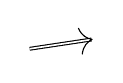
\begin{tikzpicture}\draw[->,double] (0,0)--(0.8,0.12);\end{tikzpicture}}}}

\uline{Scholium} By the bijections (34) (38), we transport onto
$\LMsourceMark{M000955}{\unsure{g}}_{\rho,\sigma},\ S_0g_{\rho,\sigma}$ the natural group structures
of $\LMsourceMark{M000956}{\unsure{\widetilde{\Gamma}_{\rho,\sigma}}},\
\LMsourceMark{M000957}{\unsure{\Gamma^{b_0}_{\rho,\sigma}}}$.
Making this group structure explicit we find in particular for $Sg_{\rho,\sigma}$
\[
\tag{\LMsourceMark{M000958}{\unsure{39|37}}}
\left\{\begin{array}{c}
(\alpha',\beta')(\alpha,\beta)=\alpha''\beta'',\quad
\text{with }\alpha''=u'(\alpha)\alpha',\quad\beta''=u'(\beta)\beta'.\\
u'=u_{\LMsourceMark{M000959}{\unsure{\zeta|\xi}}',\eta'}:\
\diagram{\begin{tikzcd}[ampersand replacement=\&,column sep=large]
\LMsourceMark{M000960}{\unsure{\mathcal{C}}}\arrow[r] \& \LMsourceMark{M000961}{\unsure{\mathcal{C}}}
\end{tikzcd}},\quad\text{defined by }
\left\{\begin{aligned}
u(\rho)&=\LMsourceMark{M000962}{\unsure{\zeta|\xi}}\rho=\operatorname{int}(\alpha)\rho\\
u(\sigma)&=\eta\sigma=\operatorname{int}(\beta)\sigma
\end{aligned}\right.
\end{array}\right.
\]
(with $\LMsourceMark{M000963}{\unsure{\zeta|\xi}}=\alpha\rho(\alpha)^{-1},\ \eta=\beta\sigma(\beta)^{-1}$).

In $\LMsourceMark{M000964}{\unsure{S_0\Gamma^{b_0}_{\rho,\sigma}}}$ we have a subgroup isomorphic to $L_0$, i.e.
\LMsourceMark{M000965}{\margin{\var{\inserted{
\[
\tag{39}
\diagram{\begin{tikzcd}[ampersand replacement=\&,column sep=large,row sep=small]
L_0\arrow[r] \& \LMsourceMark{M000966}{\unsure{S\Gamma'_{\rho,\sigma}}}\\
\LMsourceMark{M000967}{\unsure{\ell}}\arrow[r,mapsto] \& (\ell,1,1)
\end{tikzcd}}
\]
and we have exact sequence
\[
\tag{40}
\diagram{\begin{tikzcd}[ampersand replacement=\&,column sep=small]
1\arrow[r] \& L_0\arrow[r] \& \LMsourceMark{M000968}{\unsure{S\Gamma'_{\rho,\sigma}}}\arrow[r]
 \& \LMsourceMark{M000969}{\unsure{\Gamma}}_{\rho,\sigma}\arrow[r] \& 1
\end{tikzcd}}
\]
}}{\LMadded{
\[
\tag{39}
\diagram{\begin{tikzcd}[ampersand replacement=\&,column sep=large,row sep=small]
L_0\arrow[r] \& \LMsourceMark{M000970}{\unsure{S\Gamma'_{\rho,\sigma}}}\\
\LMsourceMark{M000971}{\unsure{\ell}}\arrow[r,mapsto] \& (\ell,1,1)
\end{tikzcd}}
\]
and we have exact sequence
\[
\tag{40}
\diagram{\begin{tikzcd}[ampersand replacement=\&,column sep=small]
1\arrow[r] \& L_0\arrow[r] \& \LMsourceMark{M000972}{\unsure{S\Gamma'_{\rho,\sigma}}}\arrow[r]
 \& \LMsourceMark{M000973}{\unsure{\Gamma}}_{\rho,\sigma}\arrow[r] \& 1
\end{tikzcd}}
\]
}}{insertion}{140-3-s510-I003}}}

\var{\deleted{
$\bullet$ \LMsourceMark{M000974}{\unsure{Let us now put}}
\[
\tag{39}
\begin{gathered}
M_{\rho,\sigma}\subset\operatorname{Aut}(\LMsourceMark{M000975}{\unsure{\mathcal{C}}})\\
\Vert\;\mathrm{dfn}\\
\left\{u\ \middle|\
\begin{array}{l}
\text{\LMsourceMark{M000976}{\unsure{a)|1°)}} }u\ \deleted{\LMsourceMark{M000977}{\unsure{which}}}\ \text{fixes the conjugacy classes of }\rho,\sigma\text{ in }\LMsourceMark{M000978}{\unsure{\mathcal{C}}},\\
\quad\text{i.e. }\exists\alpha_0,\beta_0\in\LMsourceMark{M000979}{\unsure{\mathcal{C}}}\ \deleted{\LMsourceMark{M000980}{\unsure{\text{such that}}}}\ \text{with }\
u(\rho)=\operatorname{int}(\alpha_0)\rho,\quad u(\sigma)=\operatorname{int}(\beta_0)\sigma,\\
\text{\LMsourceMark{M000981}{\unsure{b)|2°)}} }u\ \text{fixes the conjugacy class of }L_0,\\
\quad\text{i.e. }\exists f\in\LMsourceMark{M000982}{\unsure{\mathcal{C}}}\ \text{such that }u(L_0)=\operatorname{int}(f^{-1}).L_0,\\
\quad\text{i.e. }fu\in\operatorname{Norm}_{\operatorname{Aut}(\LMsourceMark{M000983}{\unsure{\mathcal{C}}})}(L_0)
\end{array}\right\}
\end{gathered}
\]
hence by definition of
\[
\tag{41}
\LMsourceMark{M000984}{\unsure{\mathcal{T}|\Gamma}}_{\rho,\sigma}\overset{\mathrm{dfn}}{=}
Z_\rho\mathbin{\times}_{\Gamma_{\rho,\sigma}}Z_\sigma
\]
hence
\[
\tag{42}
\diagram{\begin{tikzcd}[ampersand replacement=\&,column sep=small]
1\arrow[r] \& SZ_\rho\times SZ_\sigma\arrow[r]
 \& \LMsourceMark{M000985}{\unsure{\mathcal{T}|\Gamma}}_{\rho,\sigma}\arrow[r,"\LMsourceMark{M000986}{\unsure{\delta_{\mathcal{T}}}}"]
 \& \Gamma_{\rho,\sigma}\arrow[r] \& 1
\end{tikzcd}}
\]
}}{\LMsourceMark{M000987}{\LMcancelledDoubts{\LMsourceMark{M000988}{\unsure{Let us now put}}\quad \(\LMsourceMark{M000989}{\unsure{\mathcal{C}}}\)\quad \LMsourceMark{M000990}{\unsure{a)|1°)}}\quad \(\LMsourceMark{M000991}{\unsure{which}}\)\quad \(\LMsourceMark{M000992}{\unsure{\mathcal{C}}}\)\quad \(\LMsourceMark{M000993}{\unsure{\mathcal{C}}}\)\quad \(\LMsourceMark{M000994}{\unsure{\text{such that}}}\)\quad \LMsourceMark{M000995}{\unsure{b)|2°)}}\quad \(\LMsourceMark{M000996}{\unsure{\mathcal{C}}}\)\quad \(\LMsourceMark{M000997}{\unsure{\mathcal{C}}}\)\quad \(\LMsourceMark{M000998}{\unsure{\mathcal{T}|\Gamma}}\)\quad \(\LMsourceMark{M000999}{\unsure{\mathcal{T}|\Gamma}}\)\quad \(\LMsourceMark{M001000}{\unsure{\delta_{\mathcal{T}}}}\)}}}{deletion}{140-3-s510-D005}
\LMsourceMark{M001001}{\mspage{509}}

\LMflushnotes\LMflushpages
\ifnum\LMform=1
\begin{LMapparatus}
\LMentry{140-3-s510-D001}{deletion}{\(\deleted{\LMsourceMark{M001002}{\unsure{S\widetilde{\Gamma}^{0}_{\rho,\sigma}}}\LMsourceMark{M001003}{\unsure{=\widetilde M_{\rho,\sigma}^{0}}}\LMsourceMark{M001004}{\unsure{\subset S_0\Gamma_{\rho,\sigma}}}}\)
}{\emph{\LMomittedlabel}}{Cancelled in the manuscript: omission follows the author's final state; uncertainty in the cancelled material remains marked.}{}
\LMentry{140-3-s510-I001}{insertion}{\(\inserted{\LMsourceMark{M001005}{\unsure{S_0\Gamma^{b_0}_{\rho,\sigma}}}}\)
}{\emph{\LMinsertedlabel}}{Explicit authorial insertion: integrated at the position recorded by the transcription, without changing its reading.}{}
\LMentry{140-3-s510-D002}{deletion}{\deleted{i.e. $\LMsourceMark{M001006}{\unsure{S\Gamma'_{\rho,\sigma}}}$}
}{\emph{\LMomittedlabel}}{Cancelled in the manuscript: omission follows the author's final state; uncertainty in the cancelled material remains marked.}{}
\LMentry{140-3-s510-D003}{deletion}{\deleted{\LMsourceMark{M001007}{\unsure{here}}}
}{\emph{\LMomittedlabel}}{Cancelled in the manuscript: omission follows the author's final state; uncertainty in the cancelled material remains marked.}{}
\LMentry{140-3-s510-D004}{deletion}{\(\deleted{\LMsourceMark{M001008}{\unsure{(ua^{-1},ub^{-1})}}}\)
}{\emph{\LMomittedlabel}}{Cancelled in the manuscript: omission follows the author's final state; uncertainty in the cancelled material remains marked.}{}
\LMentry{140-3-s510-I002}{insertion}{\(\inserted{(\LMsourceMark{M001009}{\unsure{\zeta|\xi}},\eta)}\)
}{\emph{\LMinsertedlabel}}{Explicit authorial insertion: integrated at the position recorded by the transcription, without changing its reading.}{}
\LMentry{140-3-s510-I003}{insertion}{\inserted{
\[
\tag{39}
\diagram{\begin{tikzcd}[ampersand replacement=\&,column sep=large,row sep=small]
L_0\arrow[r] \& \LMsourceMark{M001010}{\unsure{S\Gamma'_{\rho,\sigma}}}\\
\LMsourceMark{M001011}{\unsure{\ell}}\arrow[r,mapsto] \& (\ell,1,1)
\end{tikzcd}}
\]
and we have exact sequence
\[
\tag{40}
\diagram{\begin{tikzcd}[ampersand replacement=\&,column sep=small]
1\arrow[r] \& L_0\arrow[r] \& \LMsourceMark{M001012}{\unsure{S\Gamma'_{\rho,\sigma}}}\arrow[r]
 \& \LMsourceMark{M001013}{\unsure{\Gamma}}_{\rho,\sigma}\arrow[r] \& 1
\end{tikzcd}}
\]
}
}{\emph{\LMinsertedlabel}}{Explicit authorial insertion: integrated at the position recorded by the transcription, without changing its reading.}{}
\LMentry{140-3-s510-D005}{deletion}{\deleted{
$\bullet$ \LMsourceMark{M001014}{\unsure{Let us now put}}
\[
\tag{39}
\begin{gathered}
M_{\rho,\sigma}\subset\operatorname{Aut}(\LMsourceMark{M001015}{\unsure{\mathcal{C}}})\\
\Vert\;\mathrm{dfn}\\
\left\{u\ \middle|\
\begin{array}{l}
\text{\LMsourceMark{M001016}{\unsure{a)|1°)}} }u\ \deleted{\LMsourceMark{M001017}{\unsure{which}}}\ \text{fixes the conjugacy classes of }\rho,\sigma\text{ in }\LMsourceMark{M001018}{\unsure{\mathcal{C}}},\\
\quad\text{i.e. }\exists\alpha_0,\beta_0\in\LMsourceMark{M001019}{\unsure{\mathcal{C}}}\ \deleted{\LMsourceMark{M001020}{\unsure{\text{such that}}}}\ \text{with }\
u(\rho)=\operatorname{int}(\alpha_0)\rho,\quad u(\sigma)=\operatorname{int}(\beta_0)\sigma,\\
\text{\LMsourceMark{M001021}{\unsure{b)|2°)}} }u\ \text{fixes the conjugacy class of }L_0,\\
\quad\text{i.e. }\exists f\in\LMsourceMark{M001022}{\unsure{\mathcal{C}}}\ \text{such that }u(L_0)=\operatorname{int}(f^{-1}).L_0,\\
\quad\text{i.e. }fu\in\operatorname{Norm}_{\operatorname{Aut}(\LMsourceMark{M001023}{\unsure{\mathcal{C}}})}(L_0)
\end{array}\right\}
\end{gathered}
\]
hence by definition of
\[
\tag{41}
\LMsourceMark{M001024}{\unsure{\mathcal{T}|\Gamma}}_{\rho,\sigma}\overset{\mathrm{dfn}}{=}
Z_\rho\mathbin{\times}_{\Gamma_{\rho,\sigma}}Z_\sigma
\]
hence
\[
\tag{42}
\diagram{\begin{tikzcd}[ampersand replacement=\&,column sep=small]
1\arrow[r] \& SZ_\rho\times SZ_\sigma\arrow[r]
 \& \LMsourceMark{M001025}{\unsure{\mathcal{T}|\Gamma}}_{\rho,\sigma}\arrow[r,"\LMsourceMark{M001026}{\unsure{\delta_{\mathcal{T}}}}"]
 \& \Gamma_{\rho,\sigma}\arrow[r] \& 1
\end{tikzcd}}
\]
}
}{\emph{\LMomittedlabel}}{Cancelled in the manuscript: omission follows the author's final state; uncertainty in the cancelled material remains marked.}{}
\end{LMapparatus}
\fi
\ifnum\LMform=2
\par\smallskip\begingroup\footnotesize\noindent\textcolor{gray}{\rule{.2\linewidth}{.35pt}}\par
\noindent\textit{\LMdoubtheading.}\par
\LMcarryover{140-3-s510-D001}{\(\LMsourceMark{M001027}{\unsure{S\widetilde{\Gamma}^{0}_{\rho,\sigma}}}\)\quad \(\LMsourceMark{M001028}{\unsure{=\widetilde M_{\rho,\sigma}^{0}}}\)\quad \(\LMsourceMark{M001029}{\unsure{\subset S_0\Gamma_{\rho,\sigma}}}\)
}
\LMcarryover{140-3-s510-D002}{\(\LMsourceMark{M001030}{\unsure{S\Gamma'_{\rho,\sigma}}}\)
}
\LMcarryover{140-3-s510-D003}{\LMsourceMark{M001031}{\unsure{here}}
}
\LMcarryover{140-3-s510-D004}{\(\LMsourceMark{M001032}{\unsure{(ua^{-1},ub^{-1})}}\)
}
\LMcarryover{140-3-s510-D005}{\LMsourceMark{M001033}{\unsure{Let us now put}}\quad \(\LMsourceMark{M001034}{\unsure{\mathcal{C}}}\)\quad \LMsourceMark{M001035}{\unsure{a)|1°)}}\quad \(\LMsourceMark{M001036}{\unsure{which}}\)\quad \(\LMsourceMark{M001037}{\unsure{\mathcal{C}}}\)\quad \(\LMsourceMark{M001038}{\unsure{\mathcal{C}}}\)\quad \(\LMsourceMark{M001039}{\unsure{\text{such that}}}\)\quad \LMsourceMark{M001040}{\unsure{b)|2°)}}\quad \(\LMsourceMark{M001041}{\unsure{\mathcal{C}}}\)\quad \(\LMsourceMark{M001042}{\unsure{\mathcal{C}}}\)\quad \(\LMsourceMark{M001043}{\unsure{\mathcal{T}|\Gamma}}\)\quad \(\LMsourceMark{M001044}{\unsure{\mathcal{T}|\Gamma}}\)\quad \(\LMsourceMark{M001045}{\unsure{\delta_{\mathcal{T}}}}\)
}
\par\endgroup\smallskip
\fi

% END PACKAGE LM_C3-492-510
\end{document}
